\begin{figure}[ht]
  \centering
    \begin{subfigure}[b]{\textwidth}
      \centering
      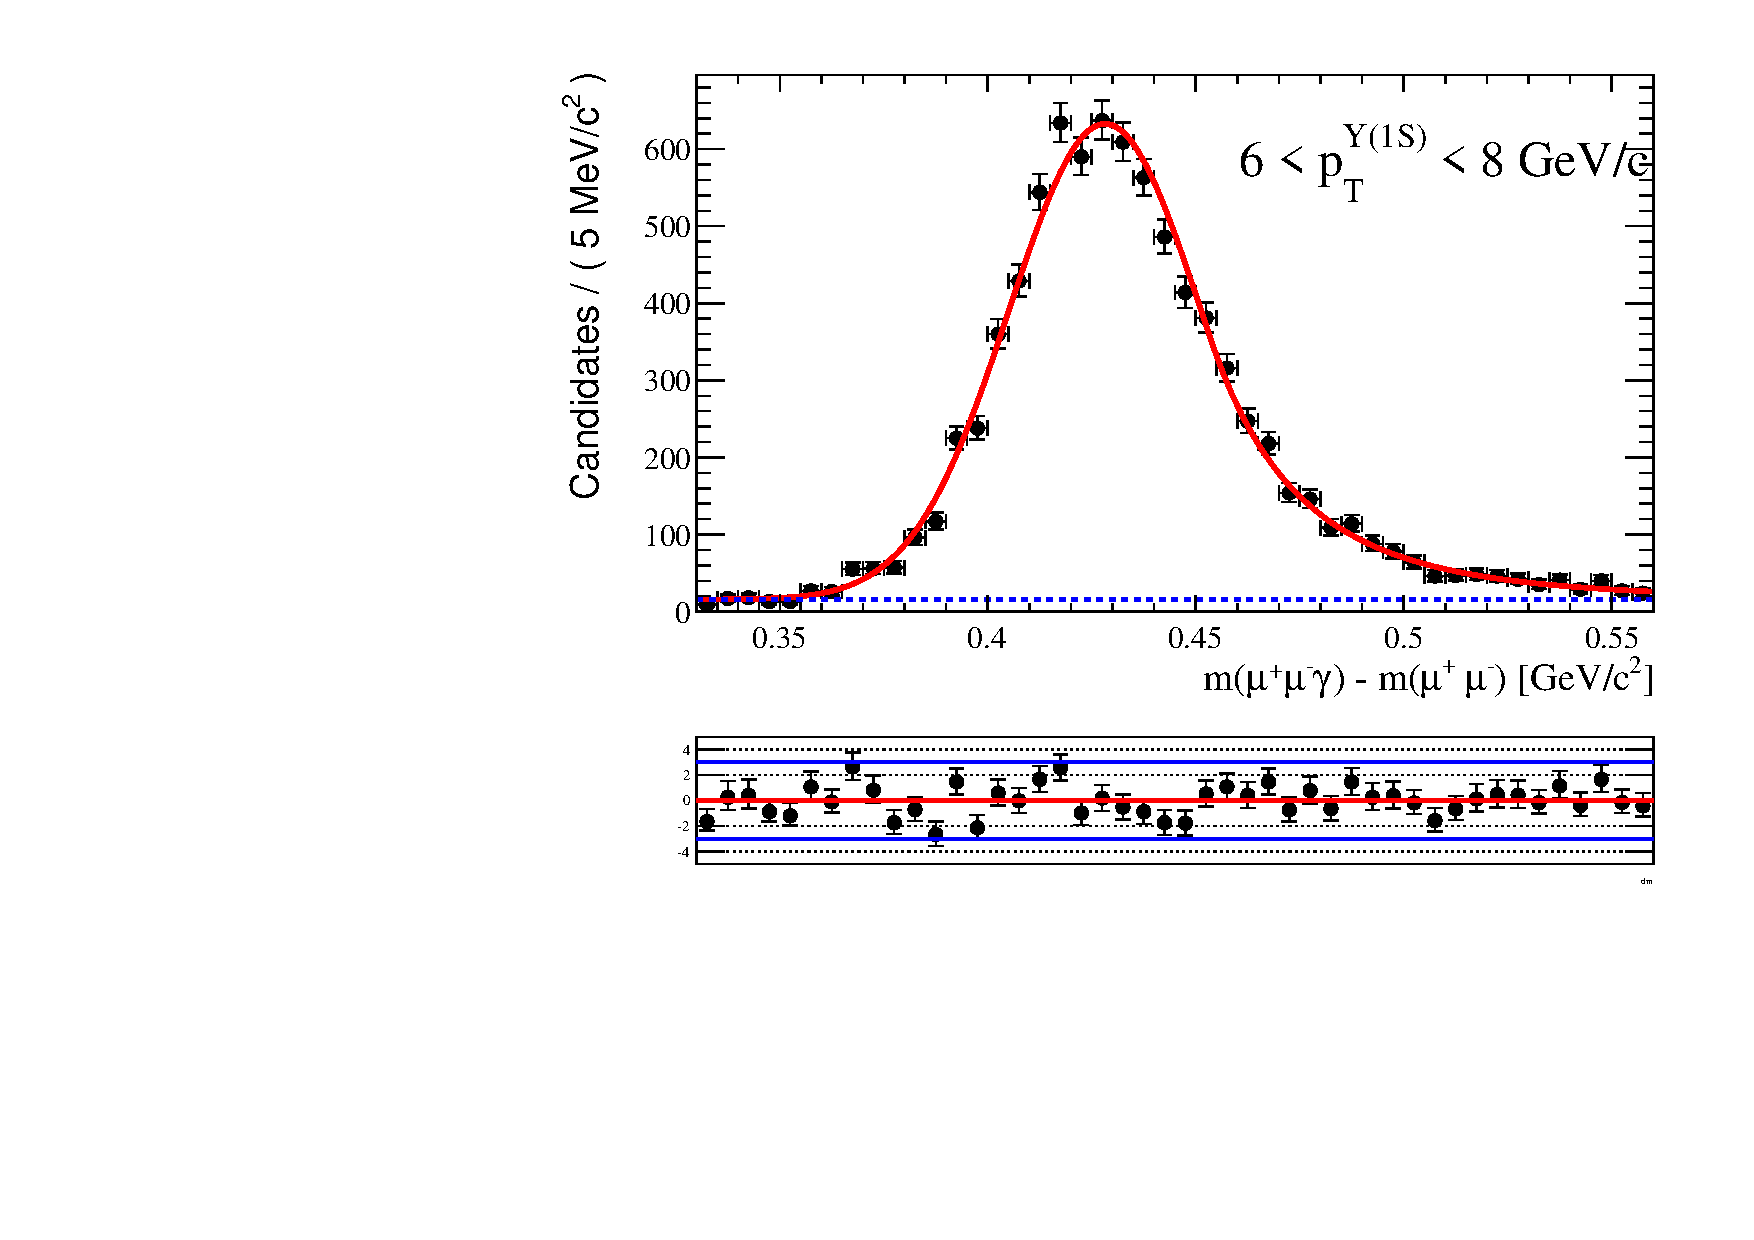
\includegraphics[width=0.16\linewidth]{fit_mc/chib11_6_8}
      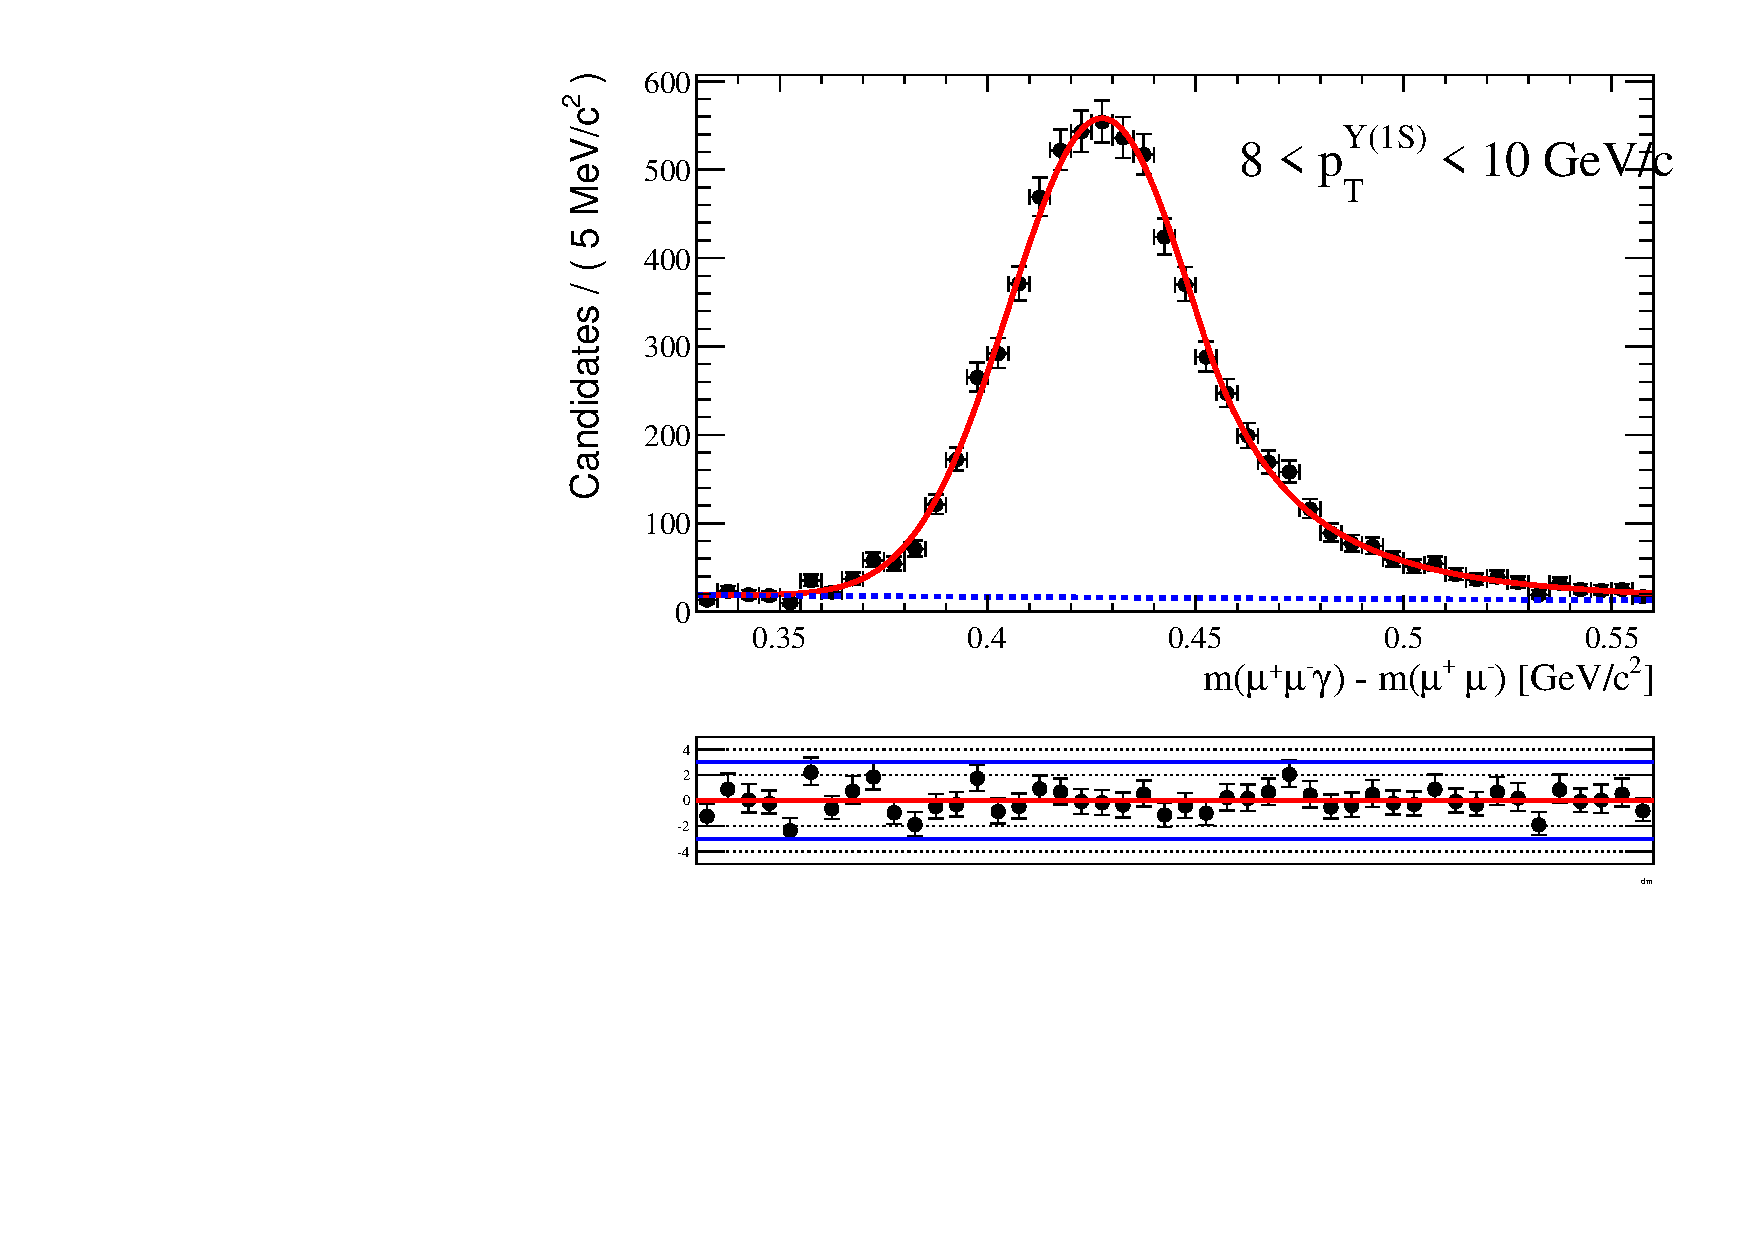
\includegraphics[width=0.16\linewidth]{fit_mc/chib11_8_10}
      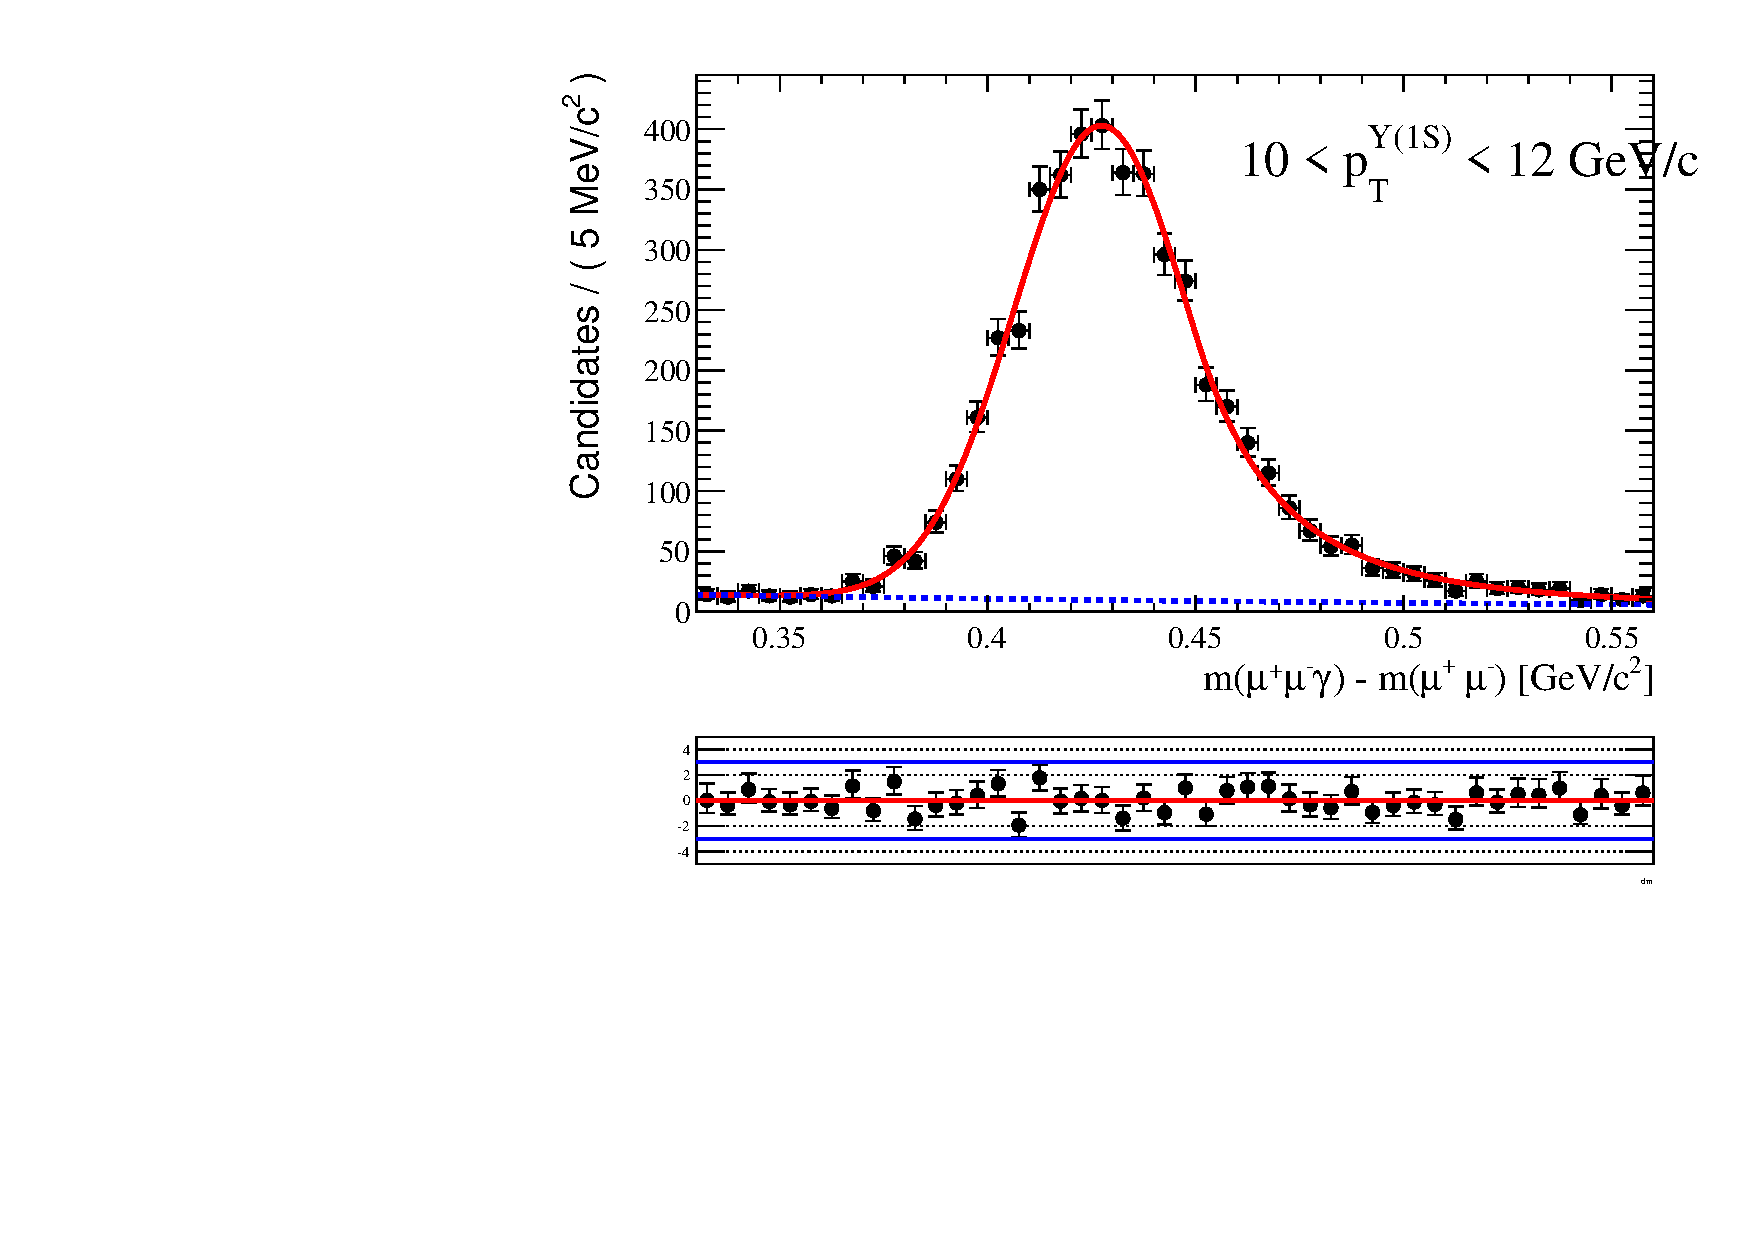
\includegraphics[width=0.16\linewidth]{fit_mc/chib11_10_12}
      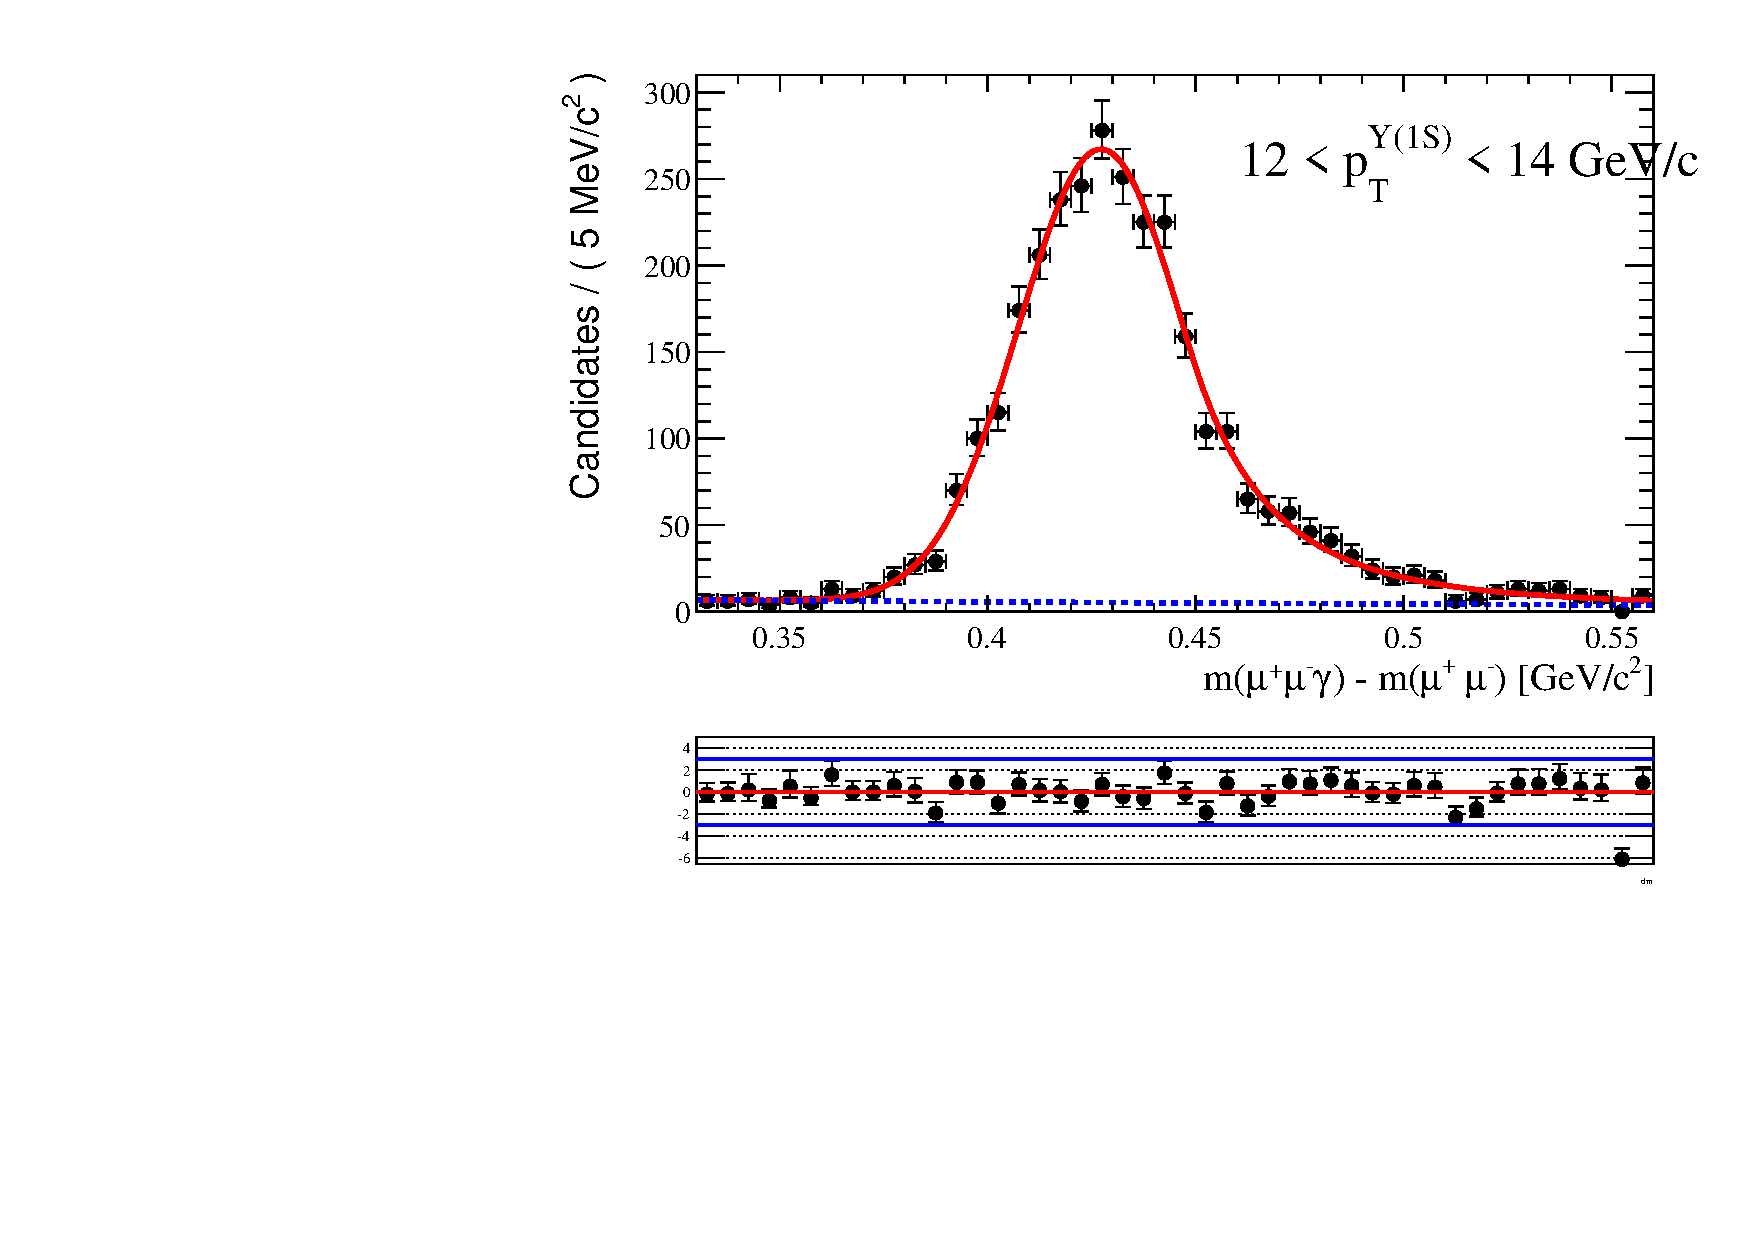
\includegraphics[width=0.16\linewidth]{fit_mc/chib11_12_14}
      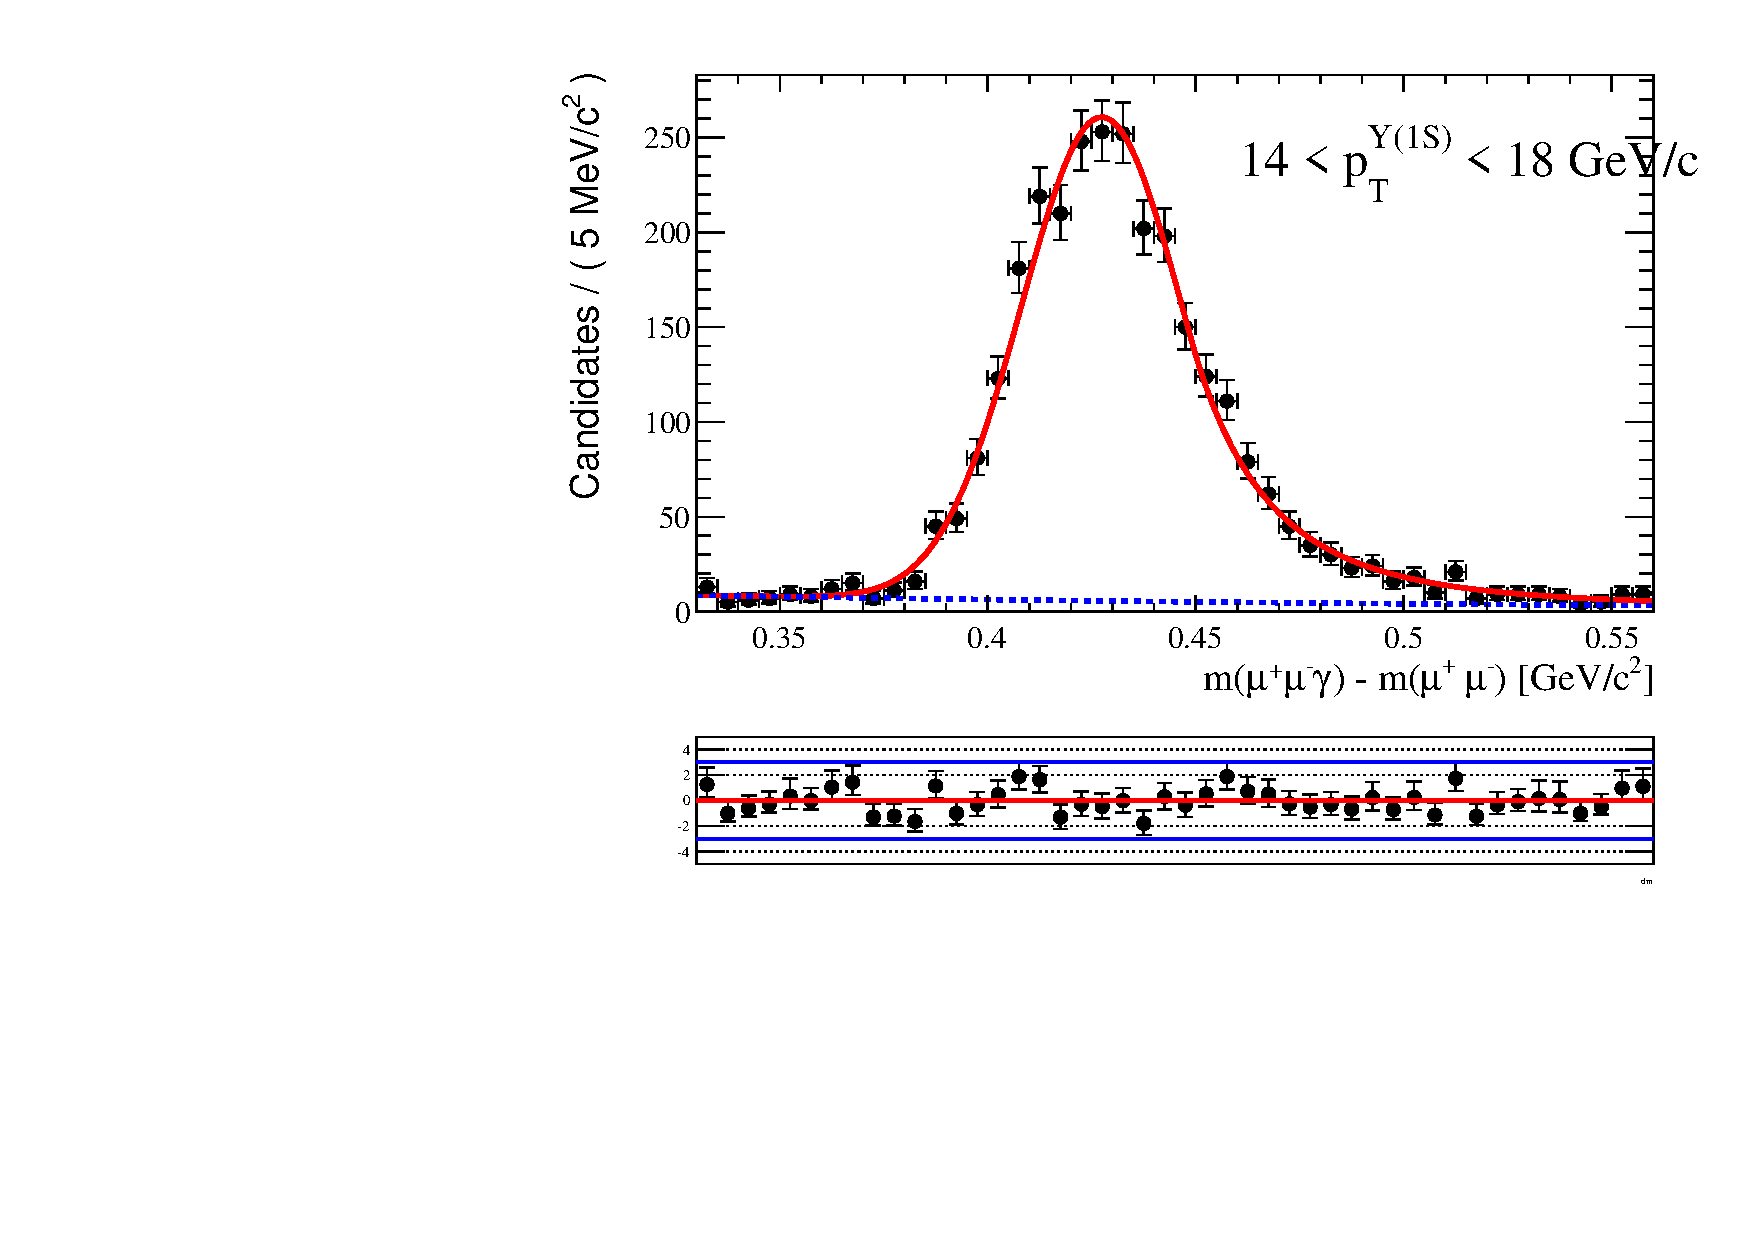
\includegraphics[width=0.16\linewidth]{fit_mc/chib11_14_18}
      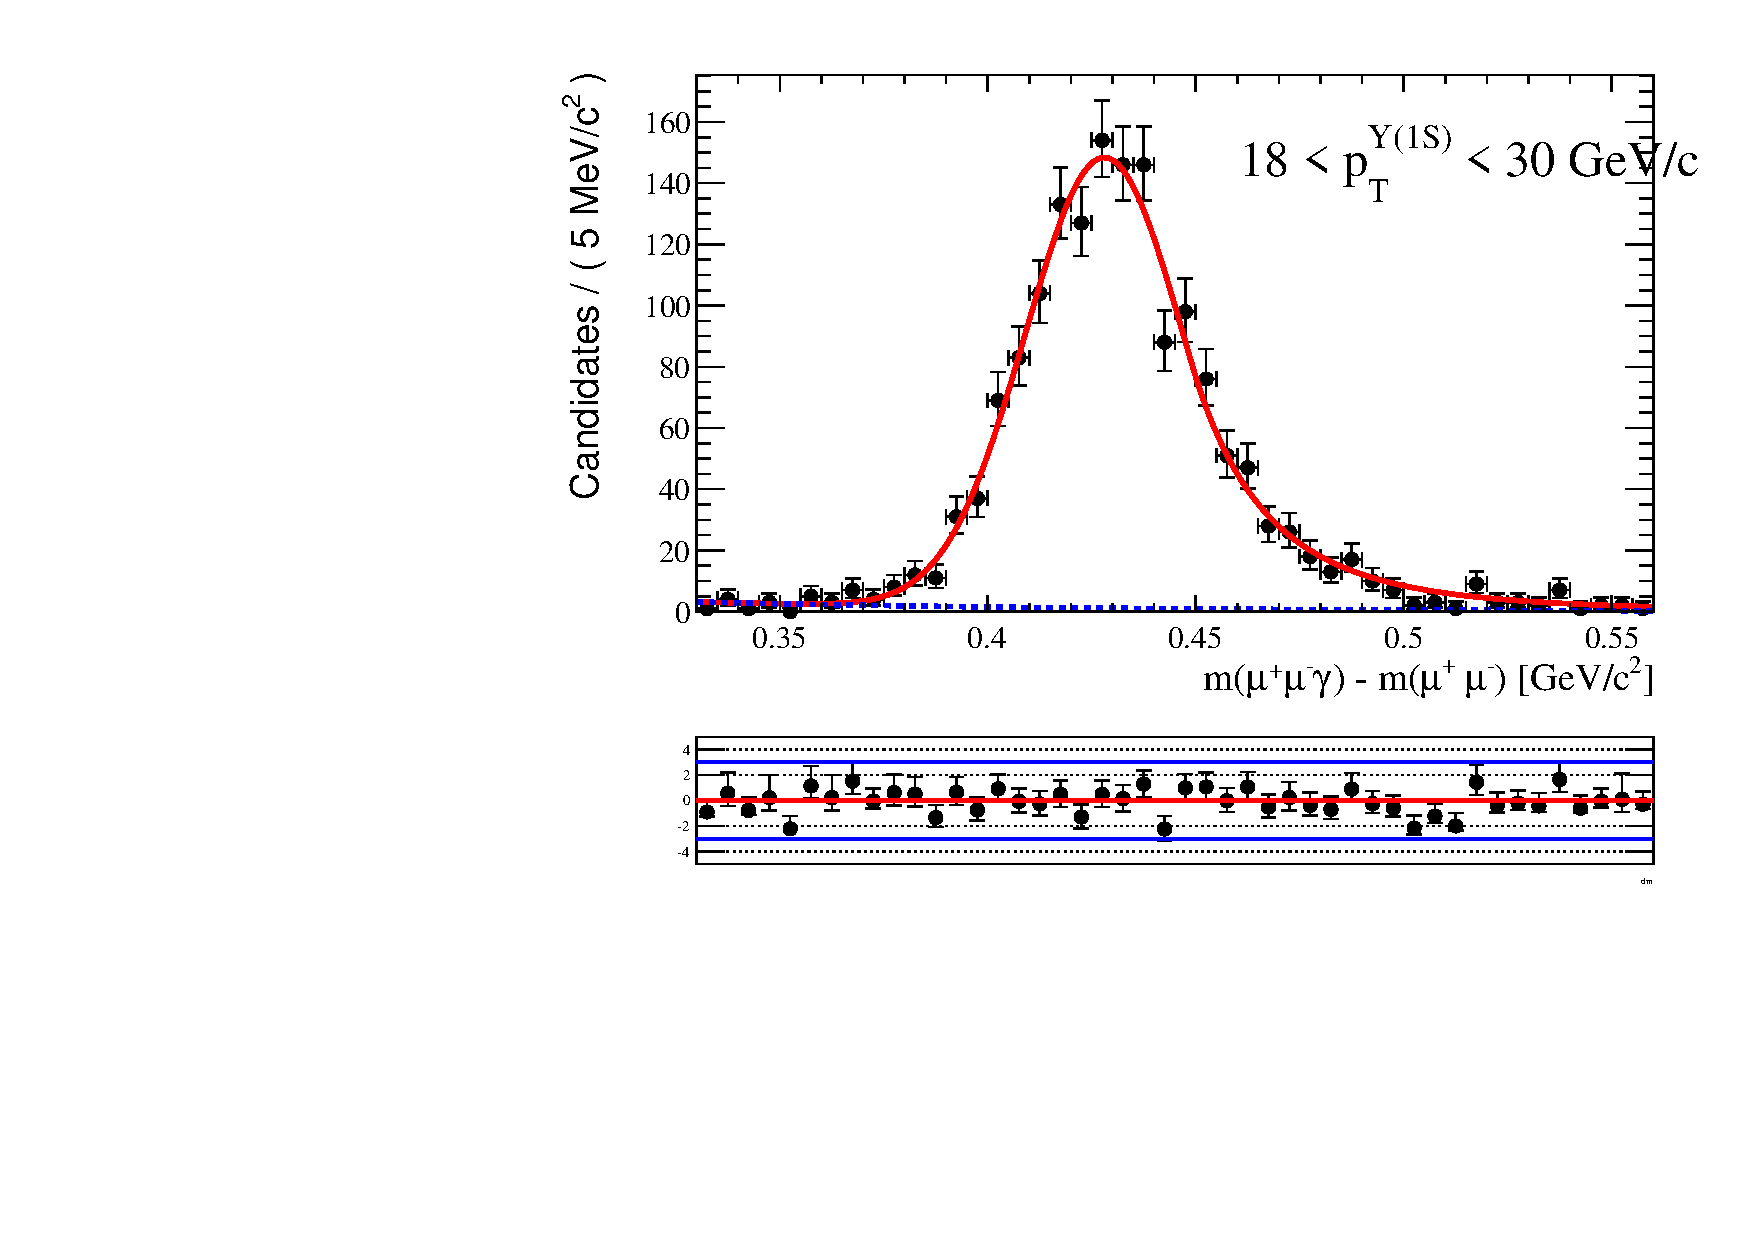
\includegraphics[width=0.16\linewidth]{fit_mc/chib11_18_30}
      \caption{\chiboneOneP}
      \label{fig:fit_mc_chiboneOneP}
    \end{subfigure}
    \begin{subfigure}[b]{\textwidth}
      \centering
      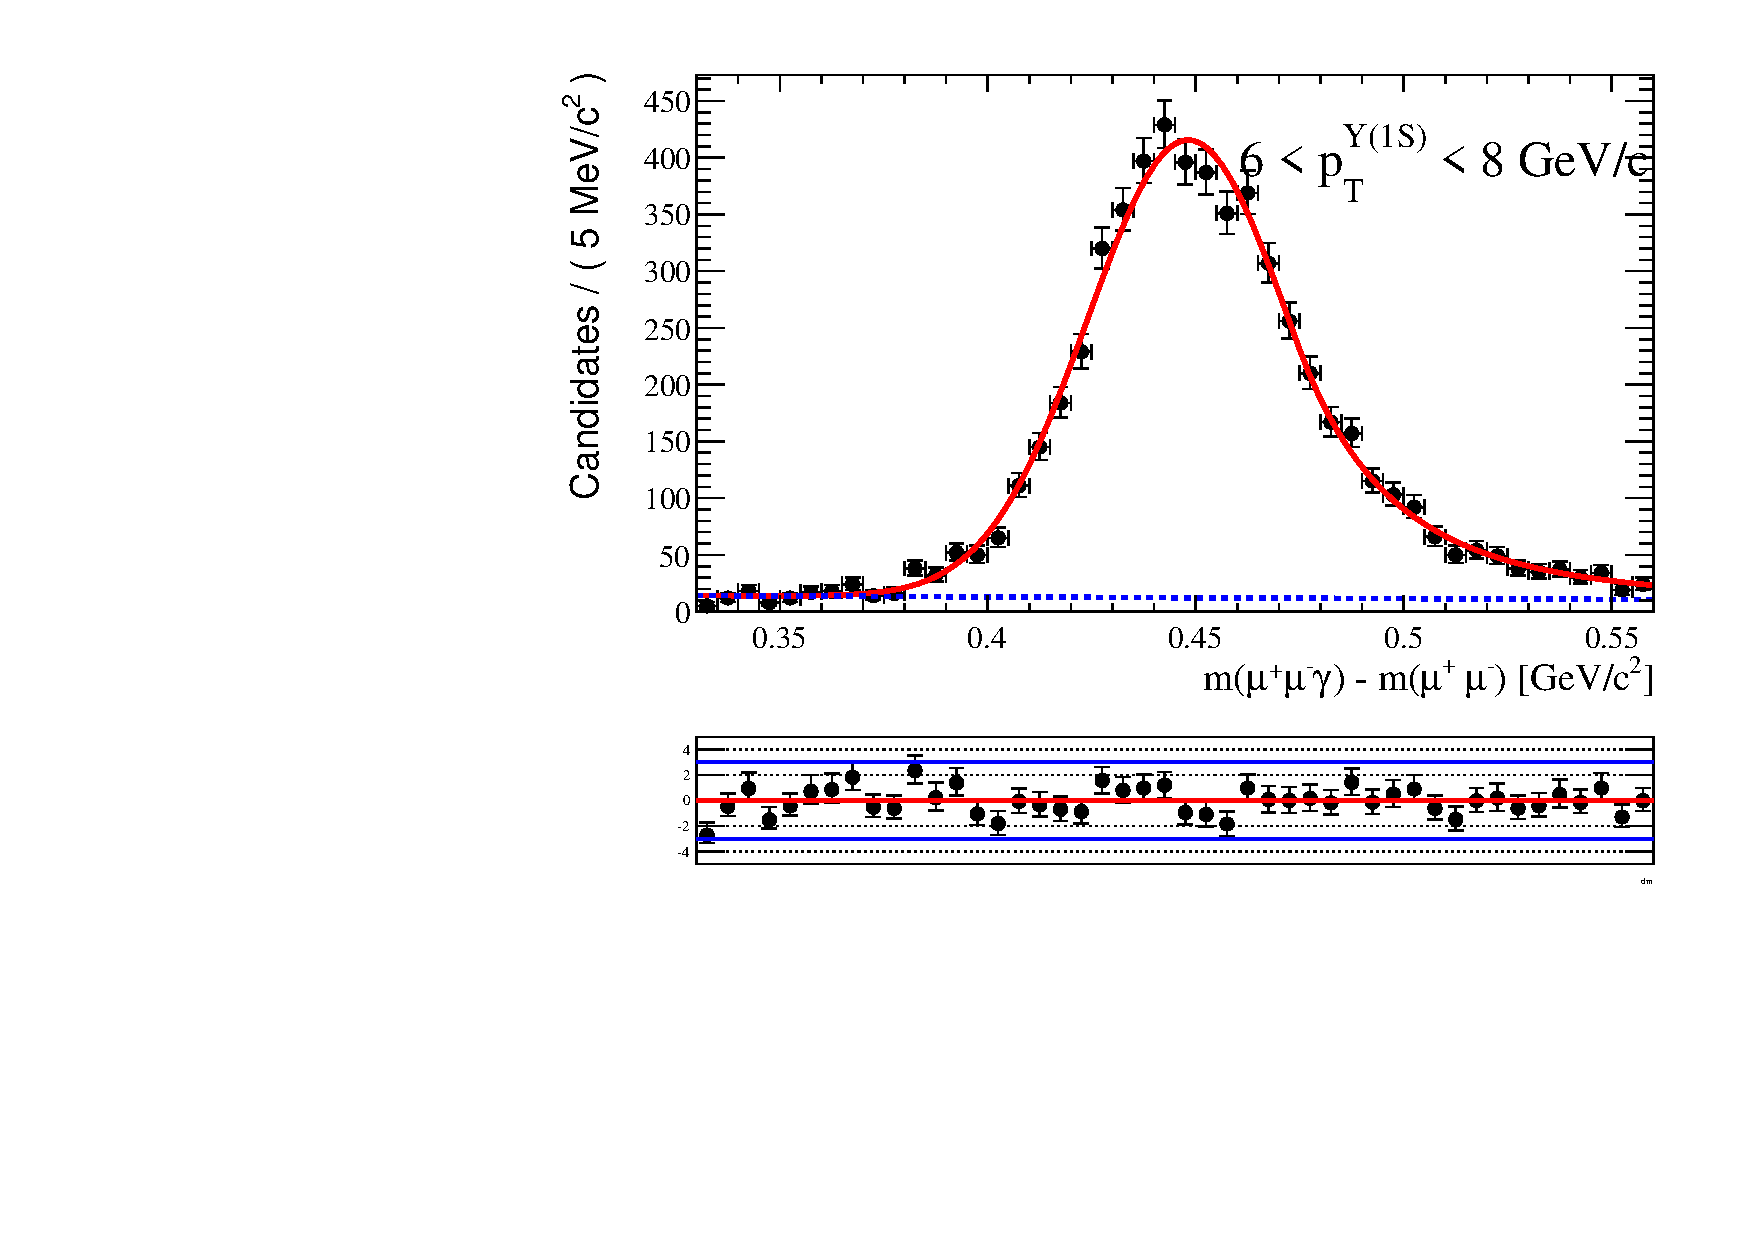
\includegraphics[width=0.16\linewidth]{fit_mc/chib21_6_8}
      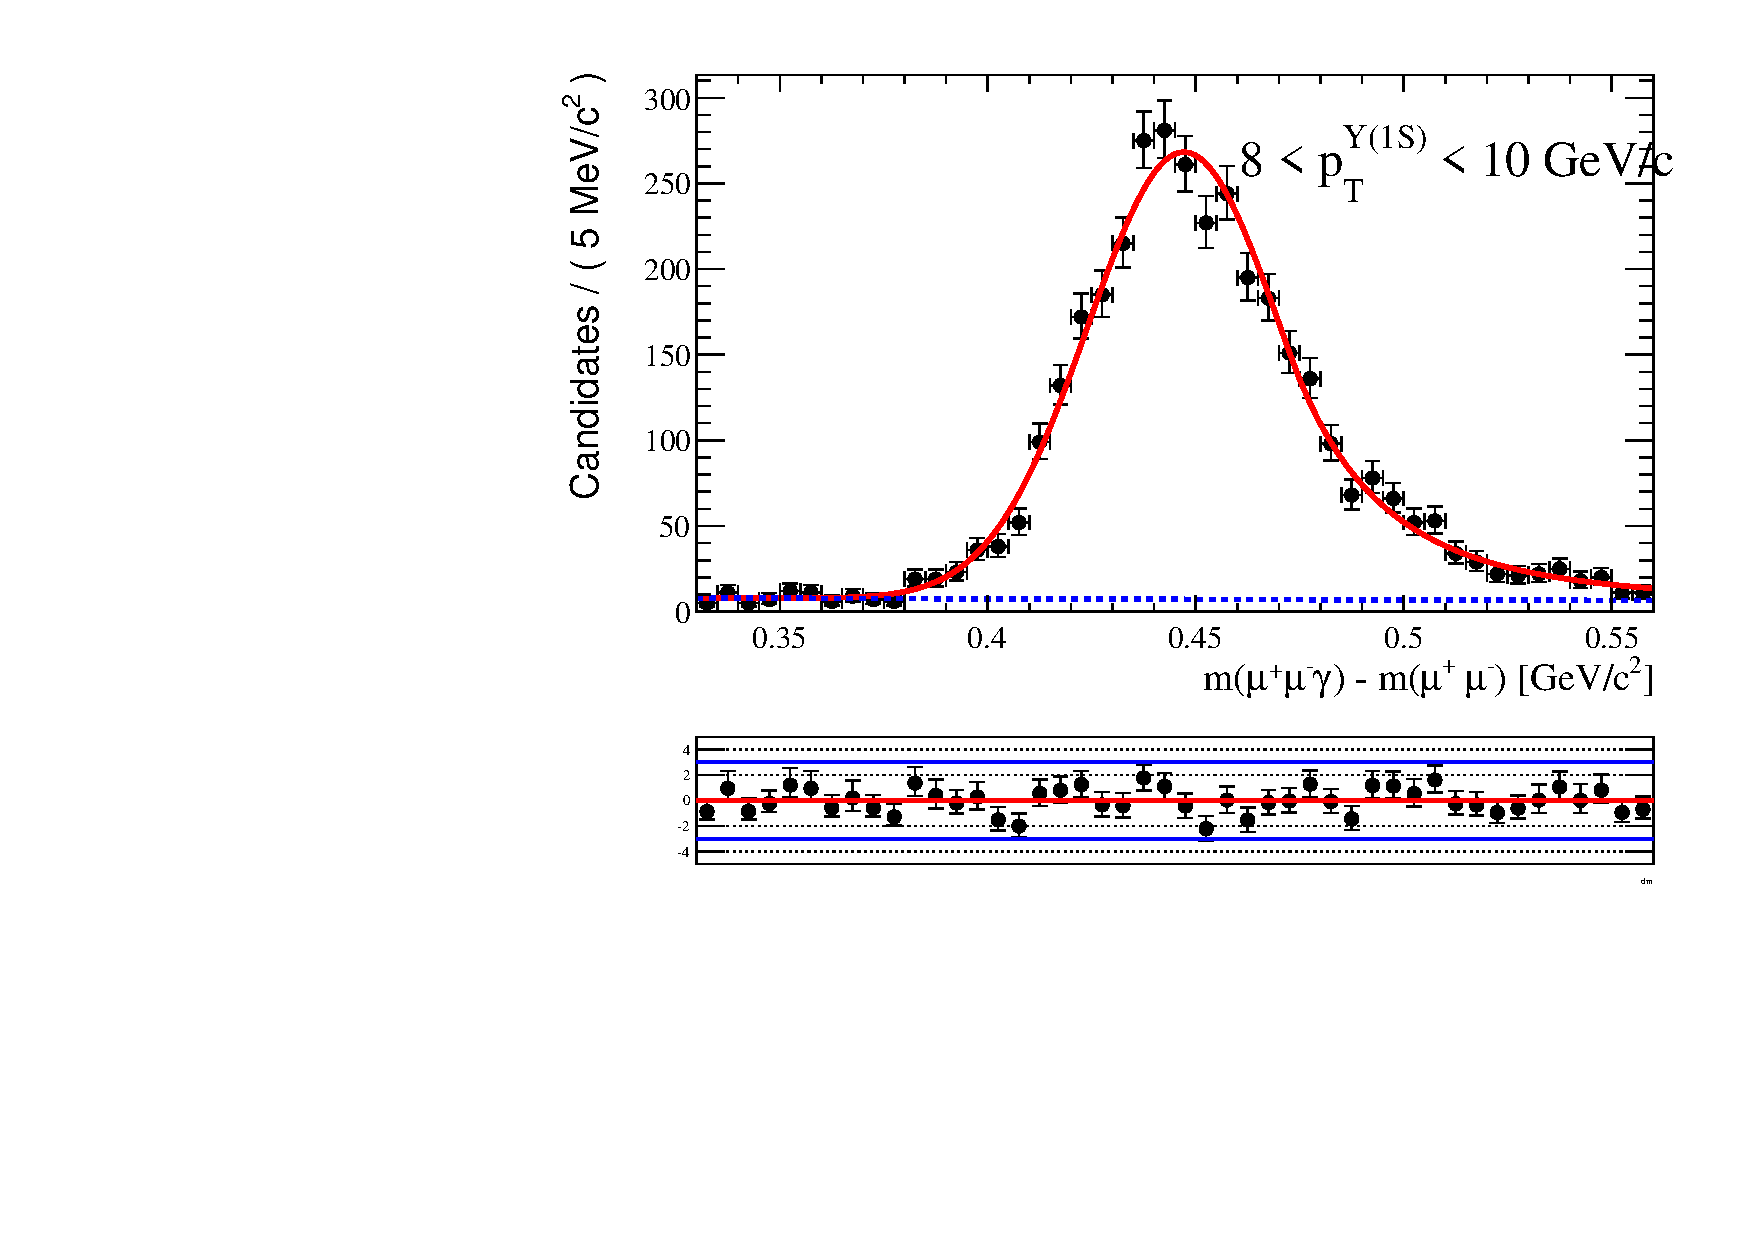
\includegraphics[width=0.16\linewidth]{fit_mc/chib21_8_10}
      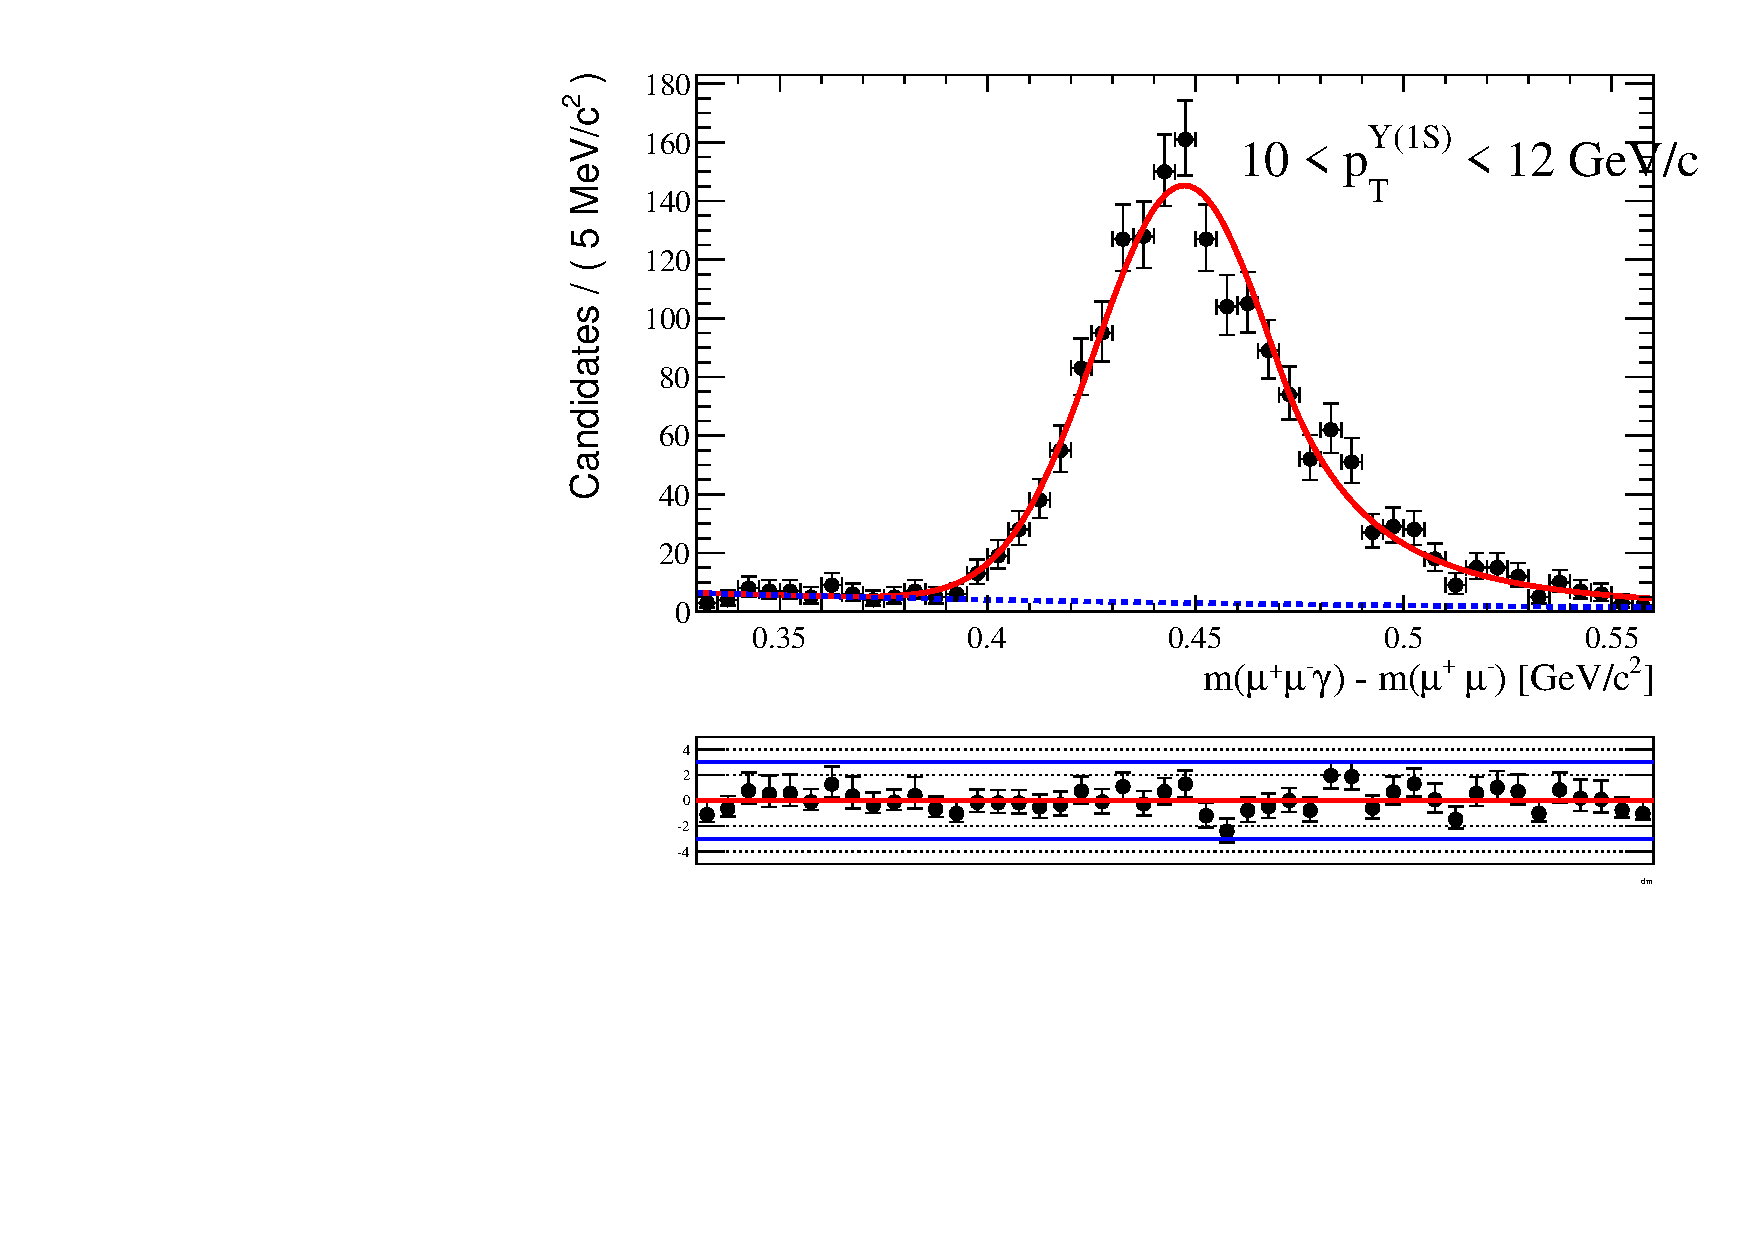
\includegraphics[width=0.16\linewidth]{fit_mc/chib21_10_12}
      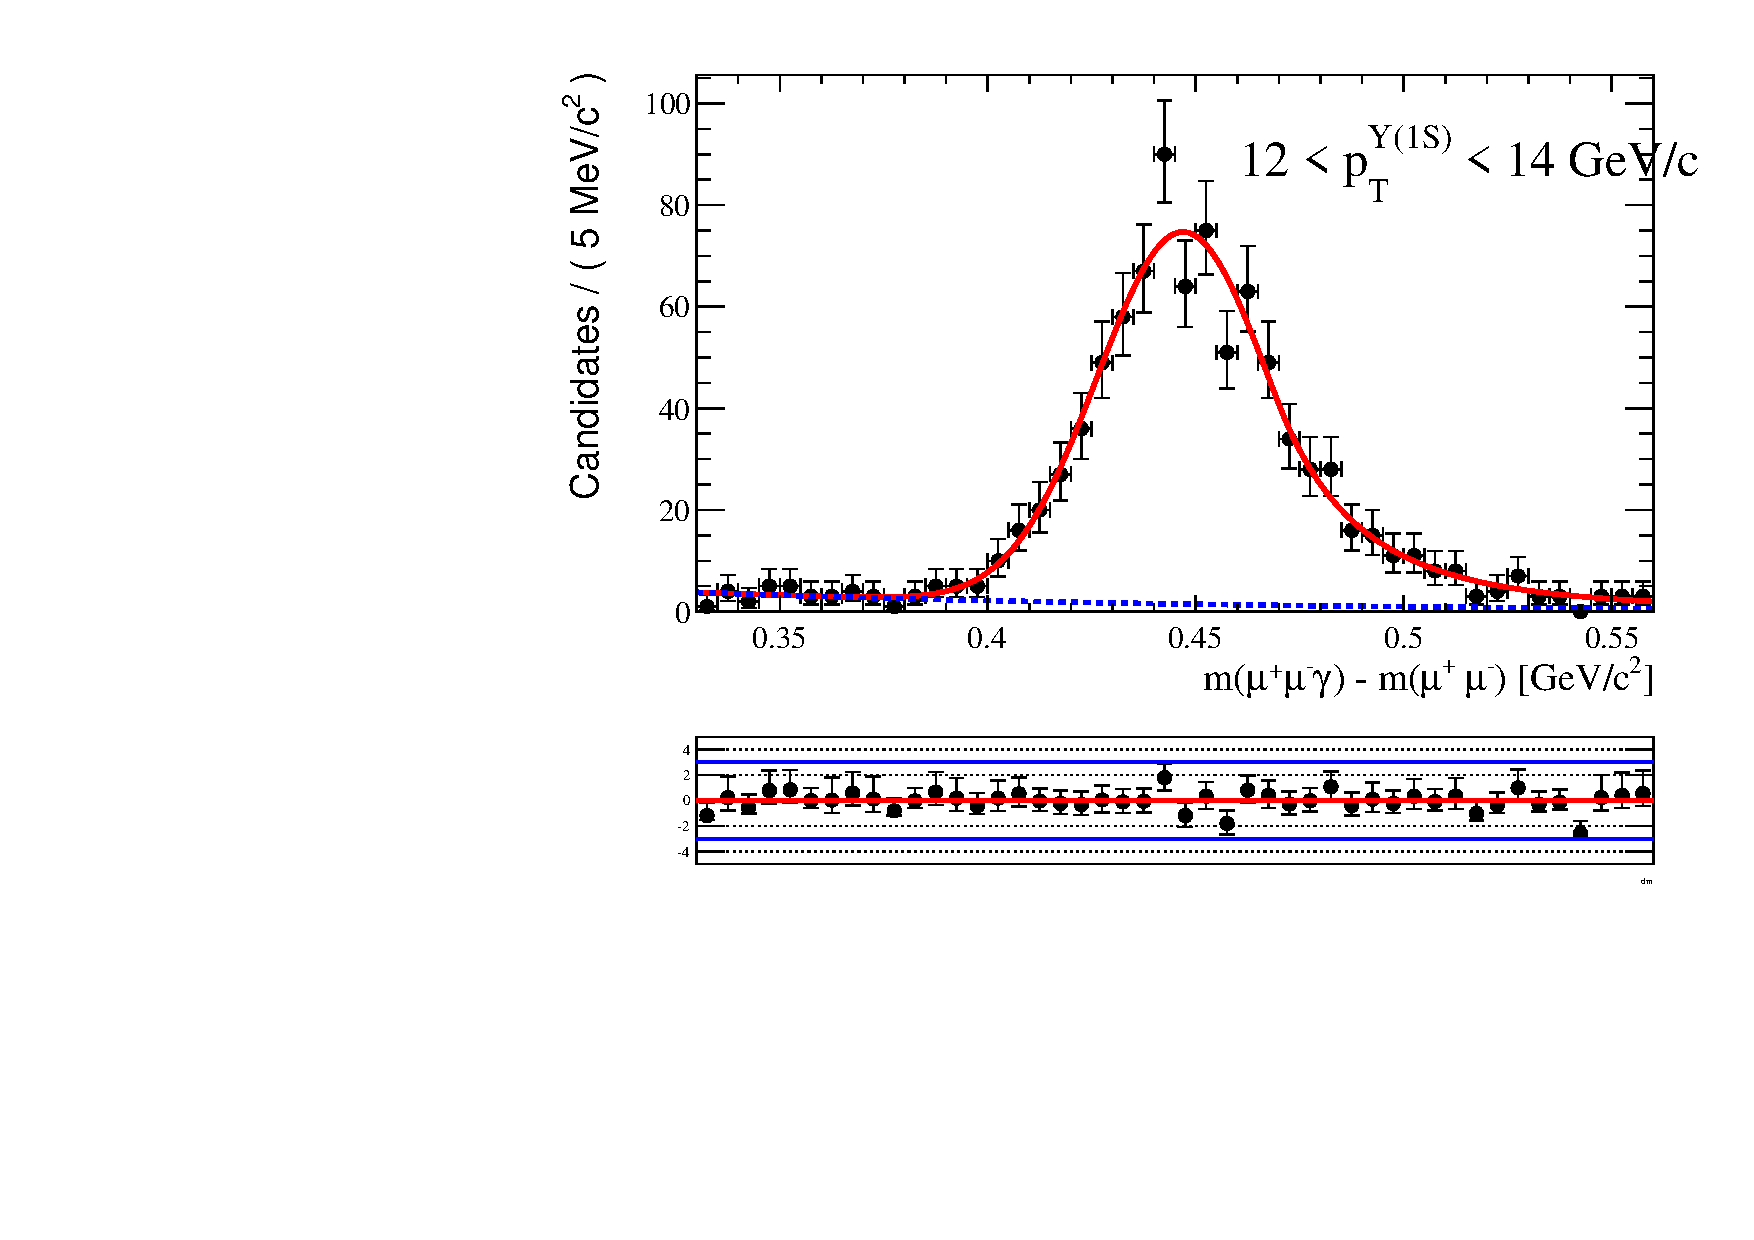
\includegraphics[width=0.16\linewidth]{fit_mc/chib21_12_14}
      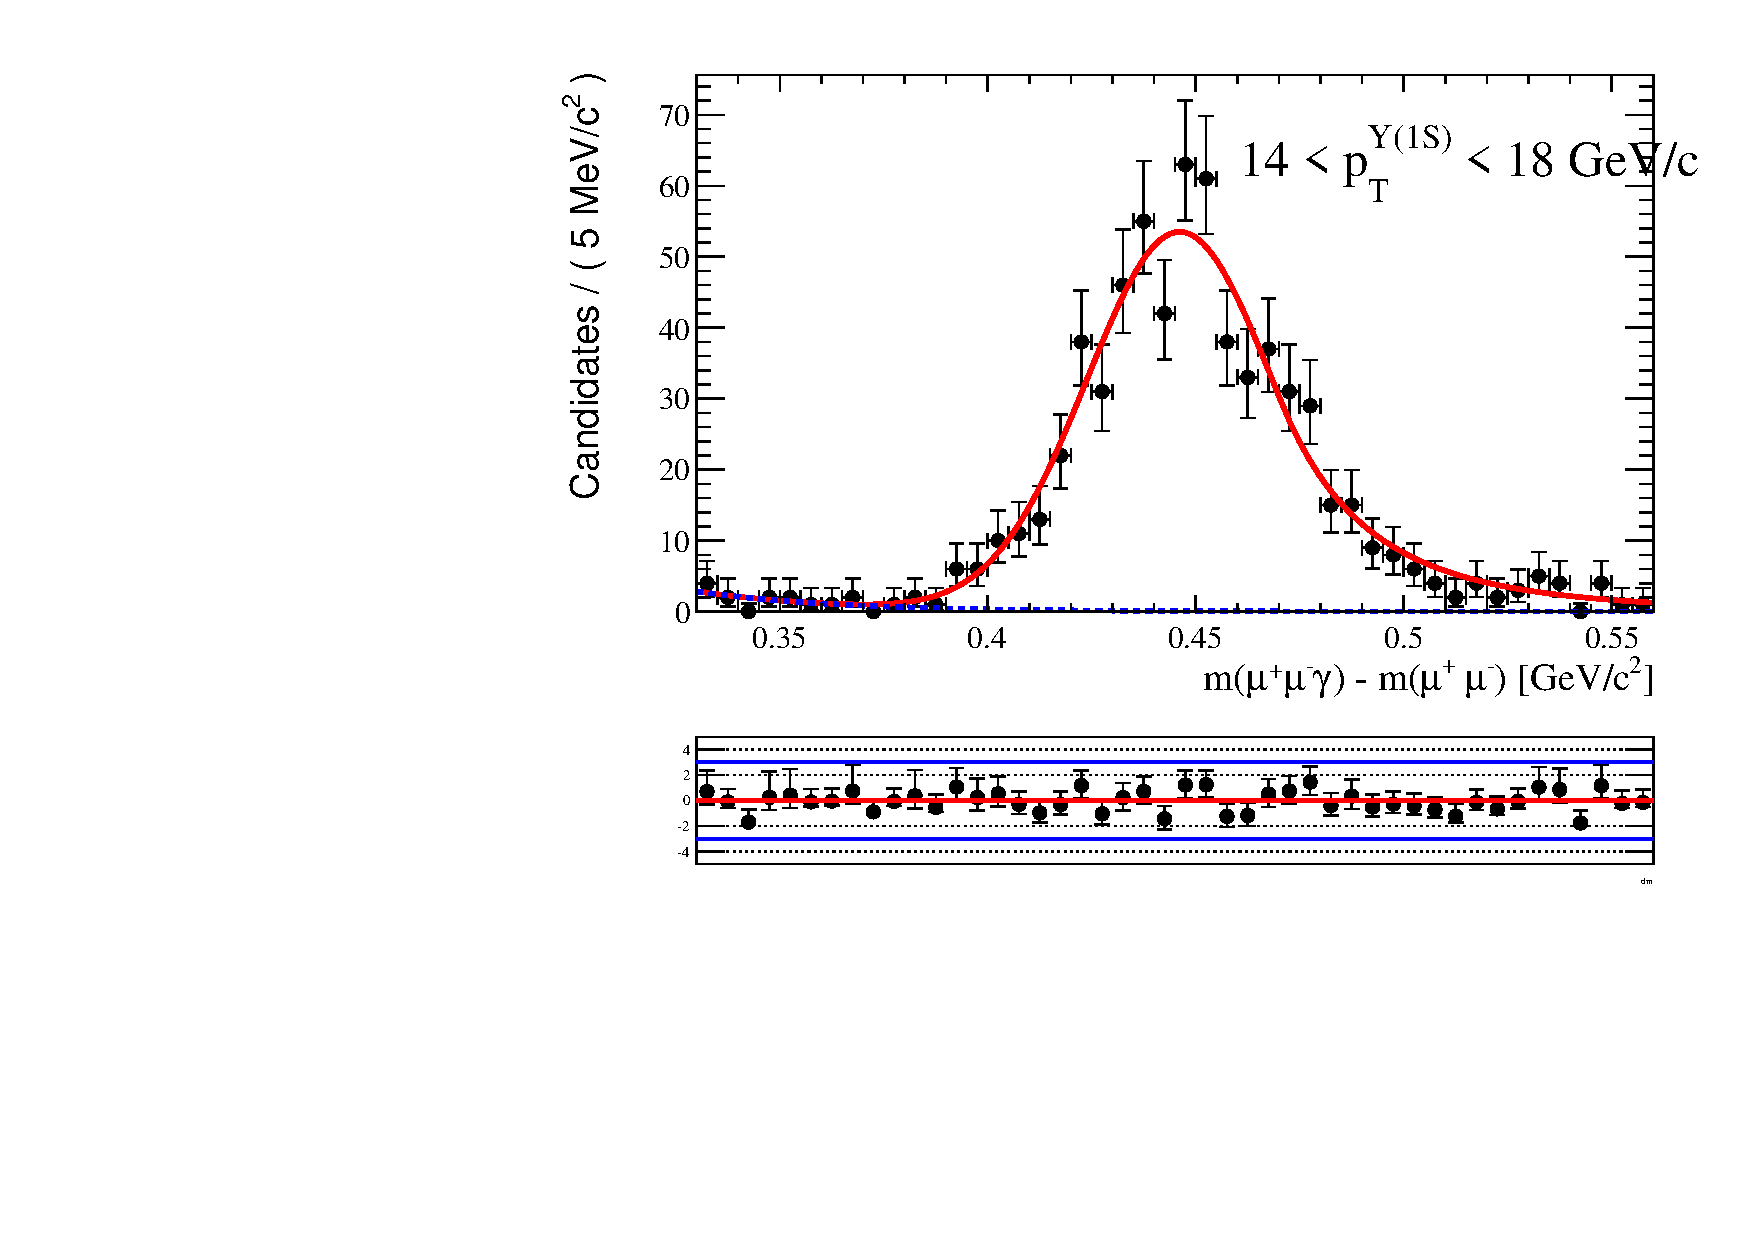
\includegraphics[width=0.16\linewidth]{fit_mc/chib21_14_18}
      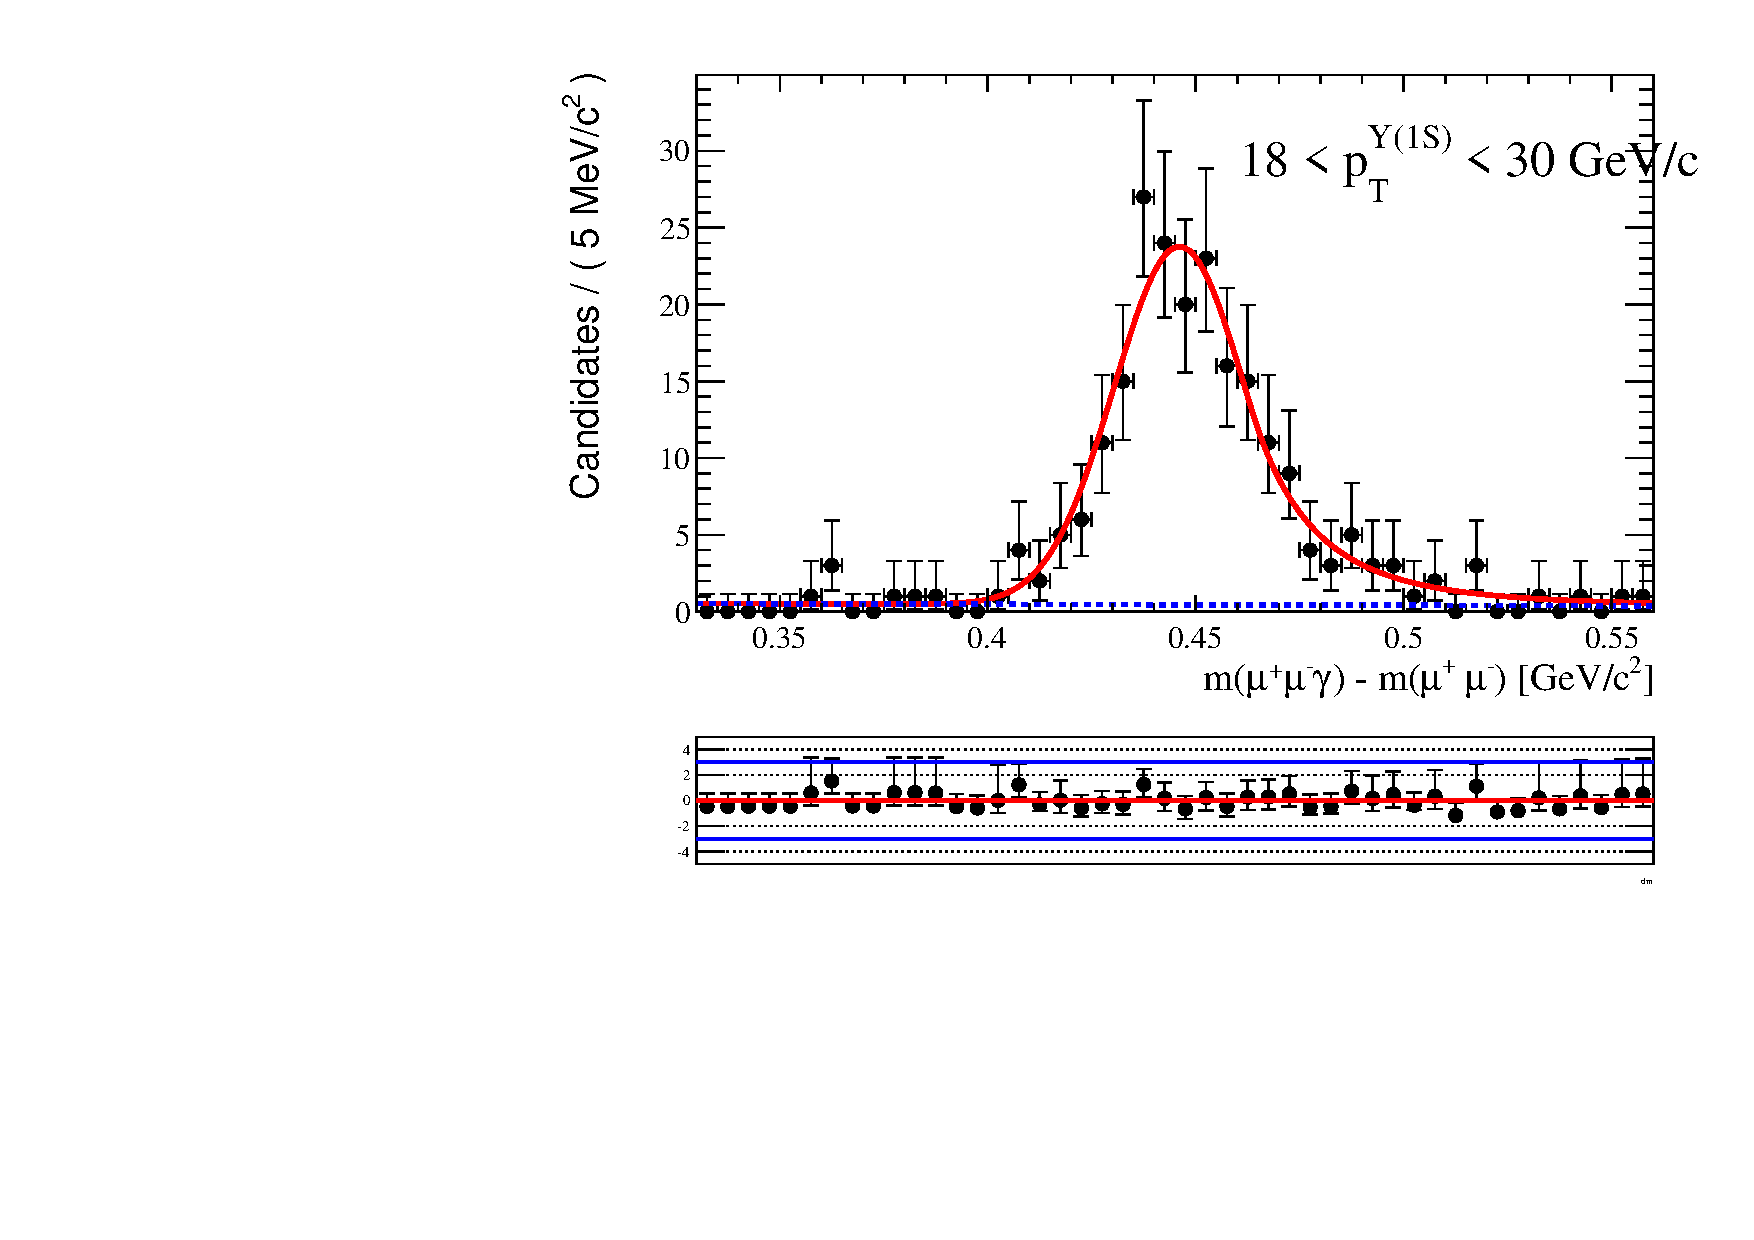
\includegraphics[width=0.16\linewidth]{fit_mc/chib21_18_30}
      \caption{\chibtwoOneP}
      \label{fig:fit_mc_chibtwoOneP}
    \end{subfigure}
    \begin{subfigure}[b]{\textwidth}
      \centering
      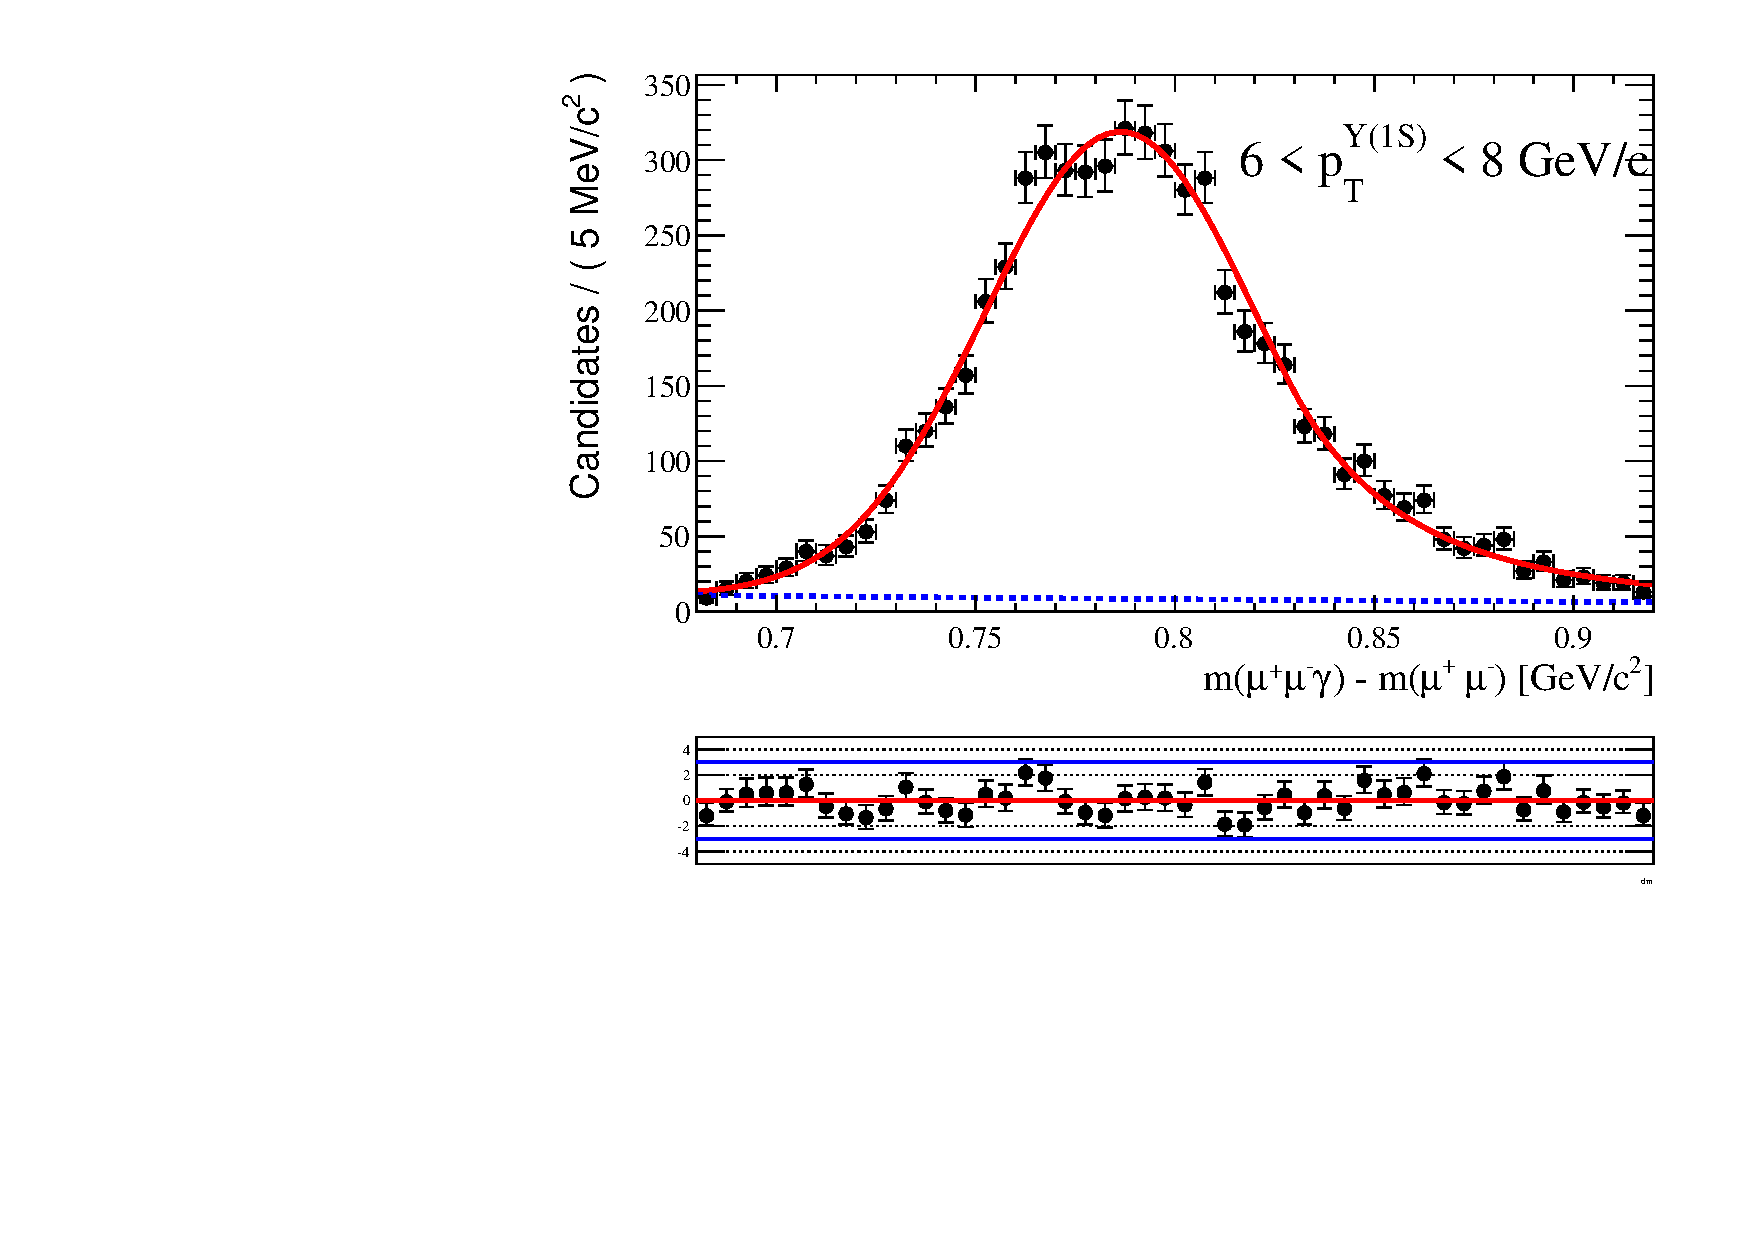
\includegraphics[width=0.16\linewidth]{fit_mc/chib12_6_8}
      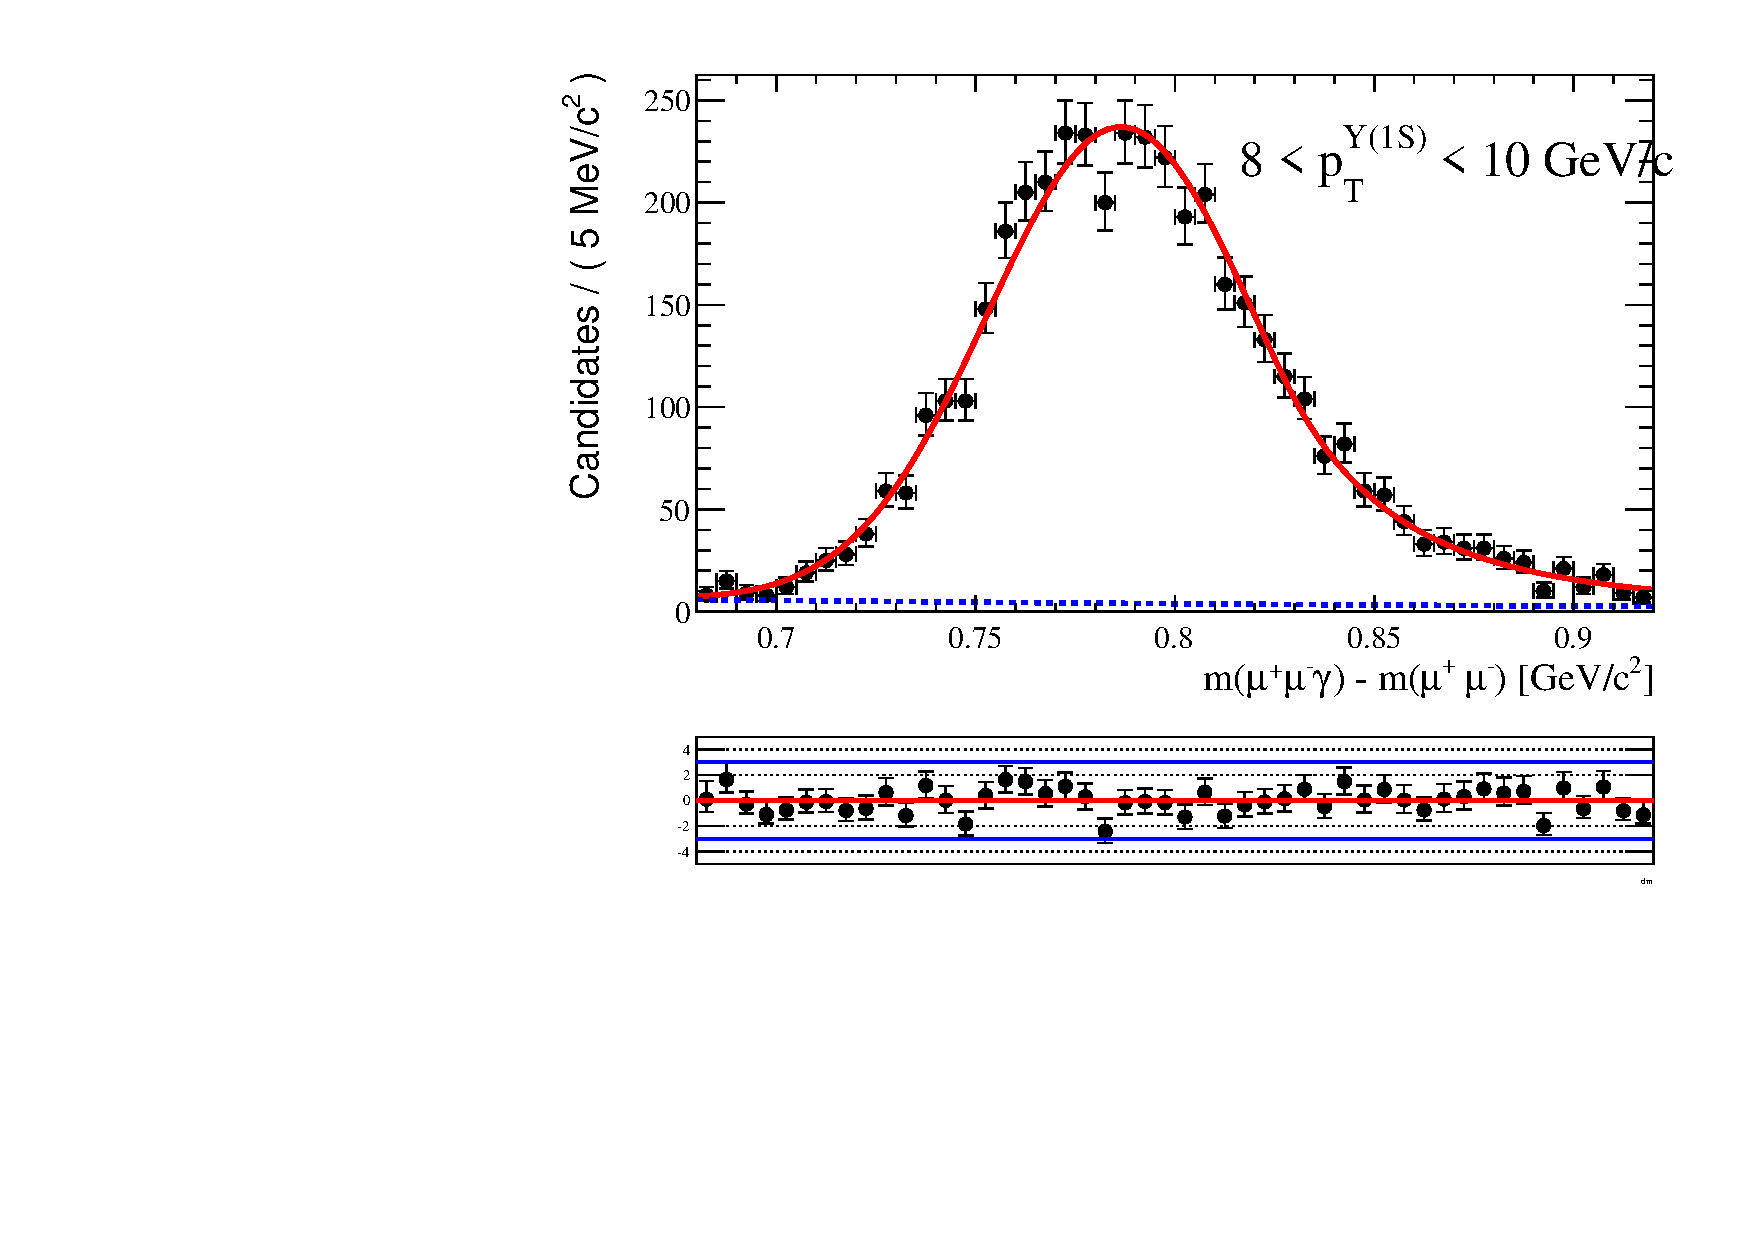
\includegraphics[width=0.16\linewidth]{fit_mc/chib12_8_10}
      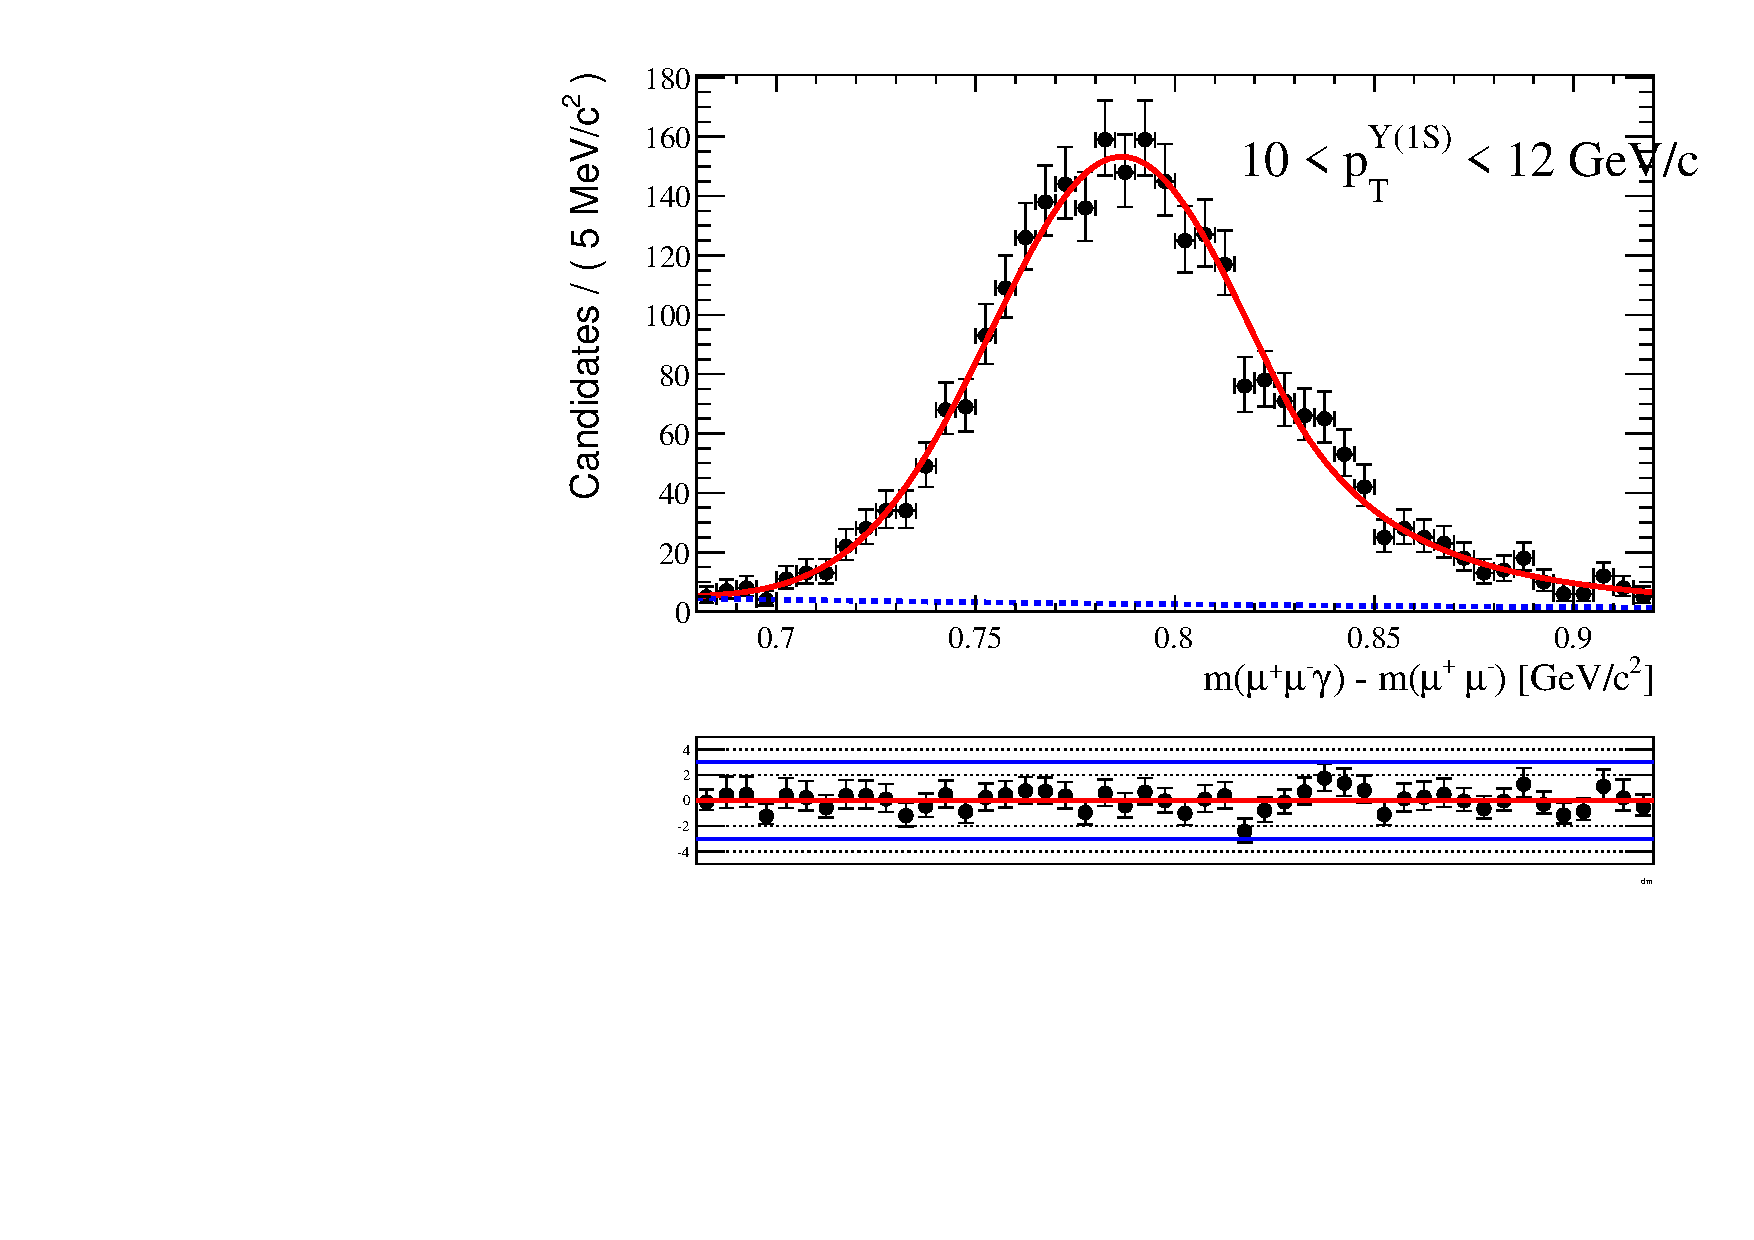
\includegraphics[width=0.16\linewidth]{fit_mc/chib12_10_12}
      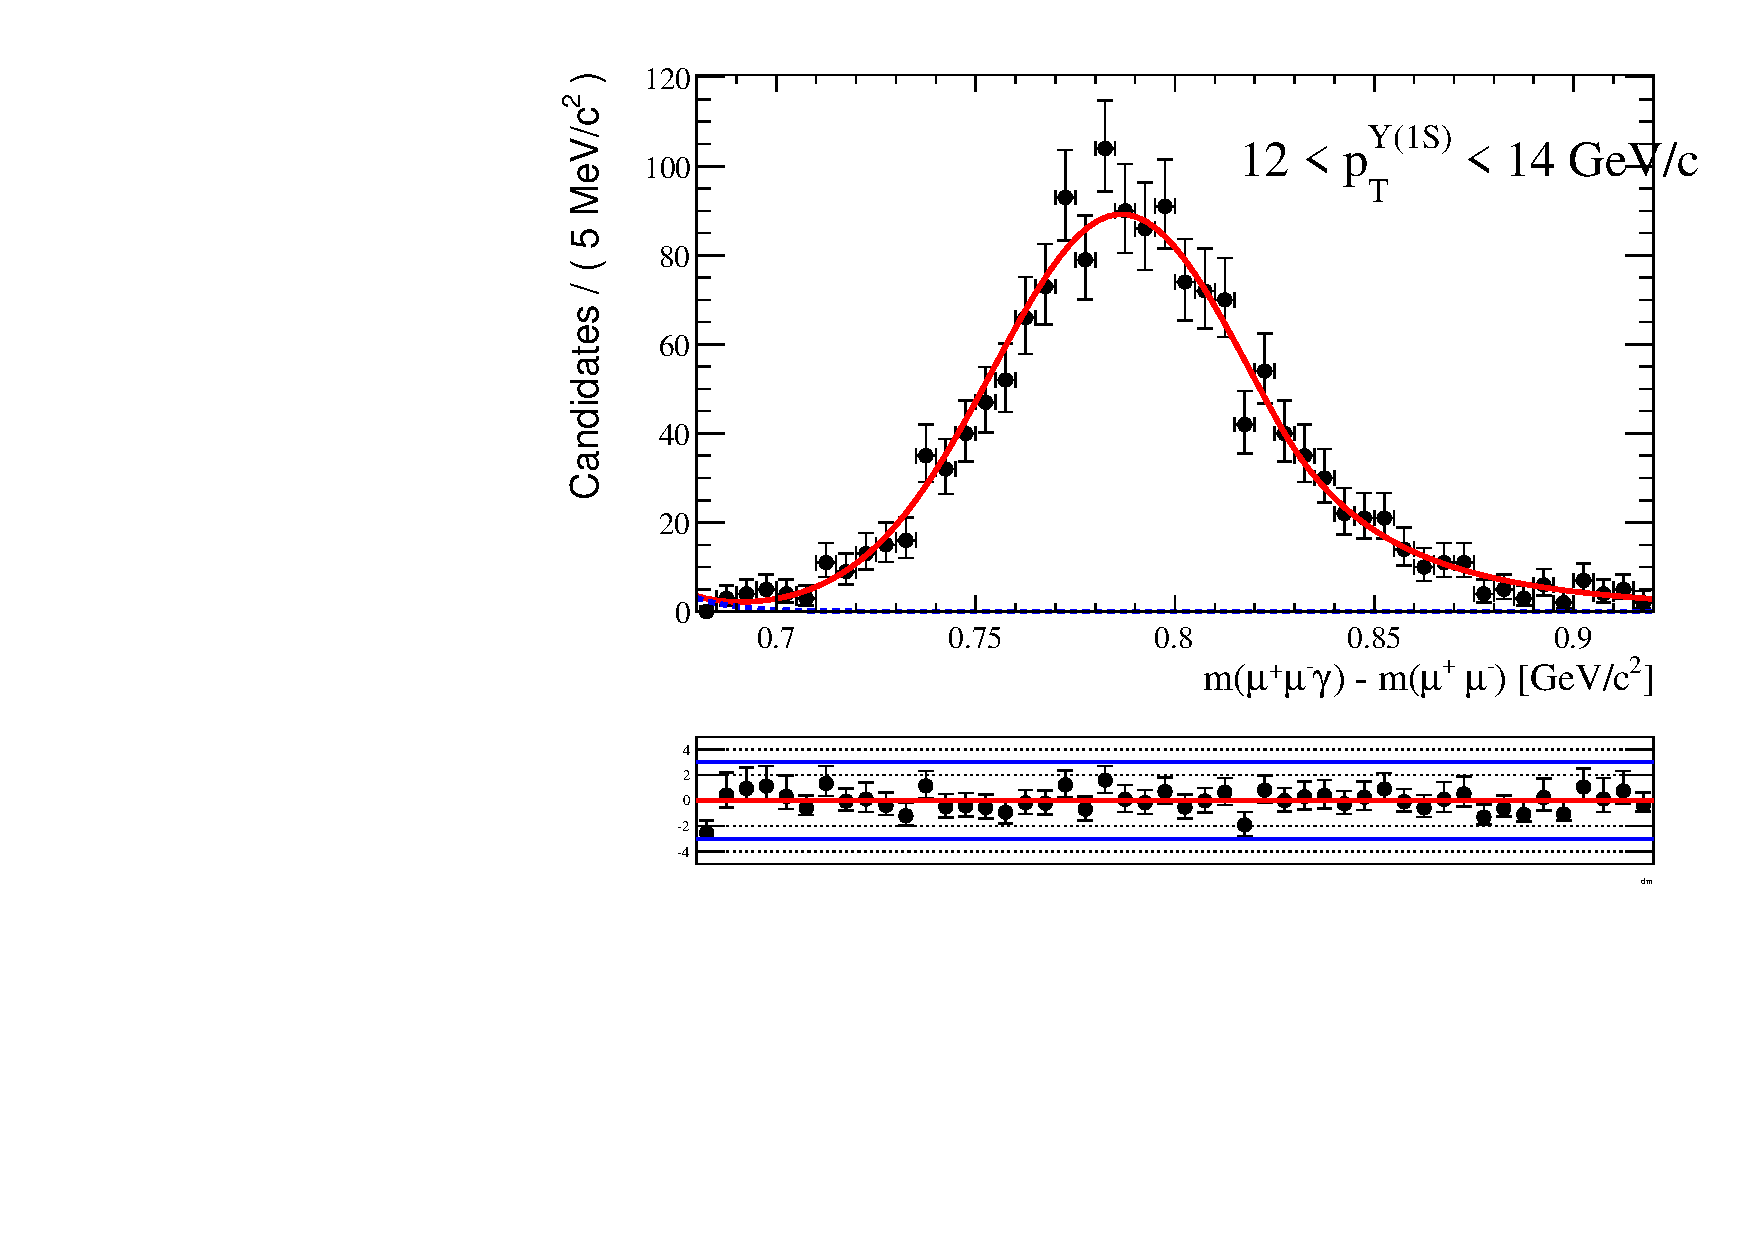
\includegraphics[width=0.16\linewidth]{fit_mc/chib12_12_14}
      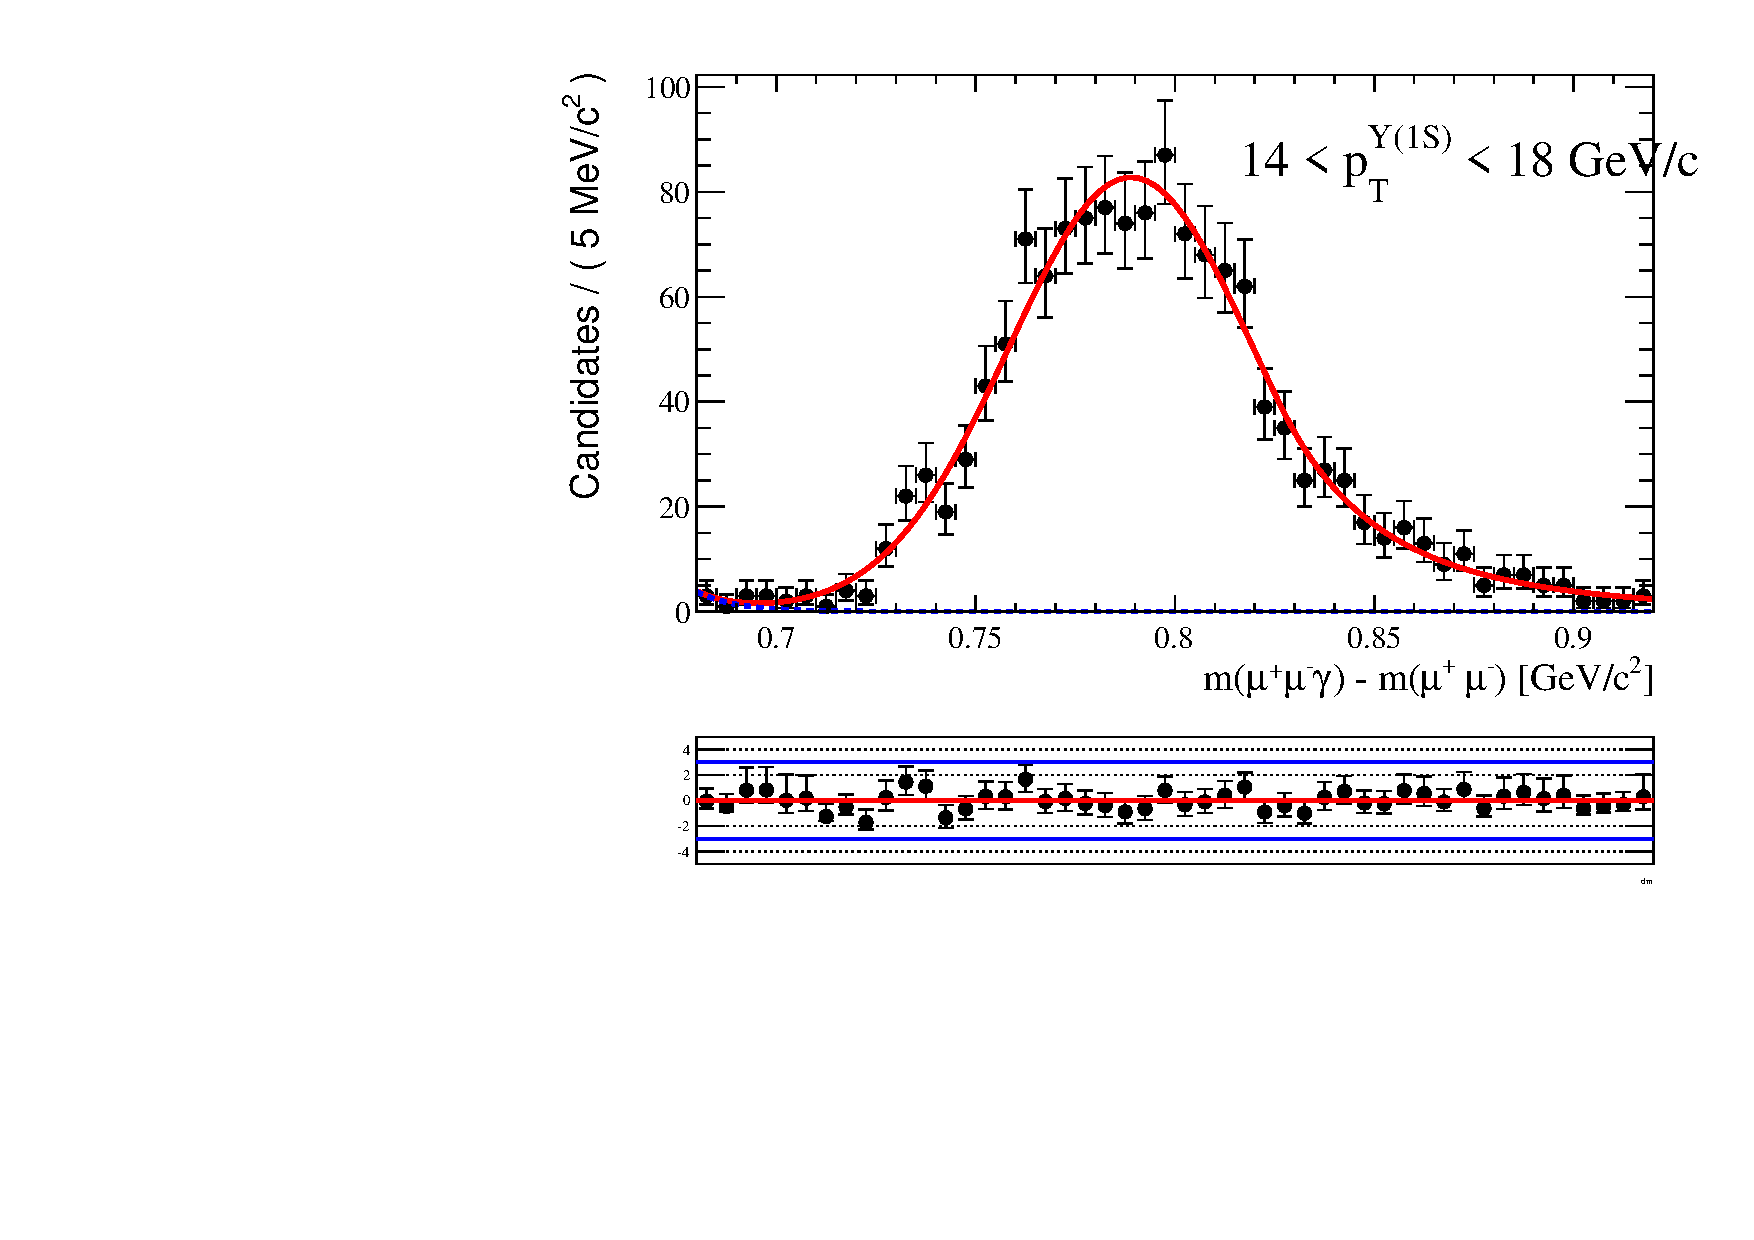
\includegraphics[width=0.16\linewidth]{fit_mc/chib12_14_18}
      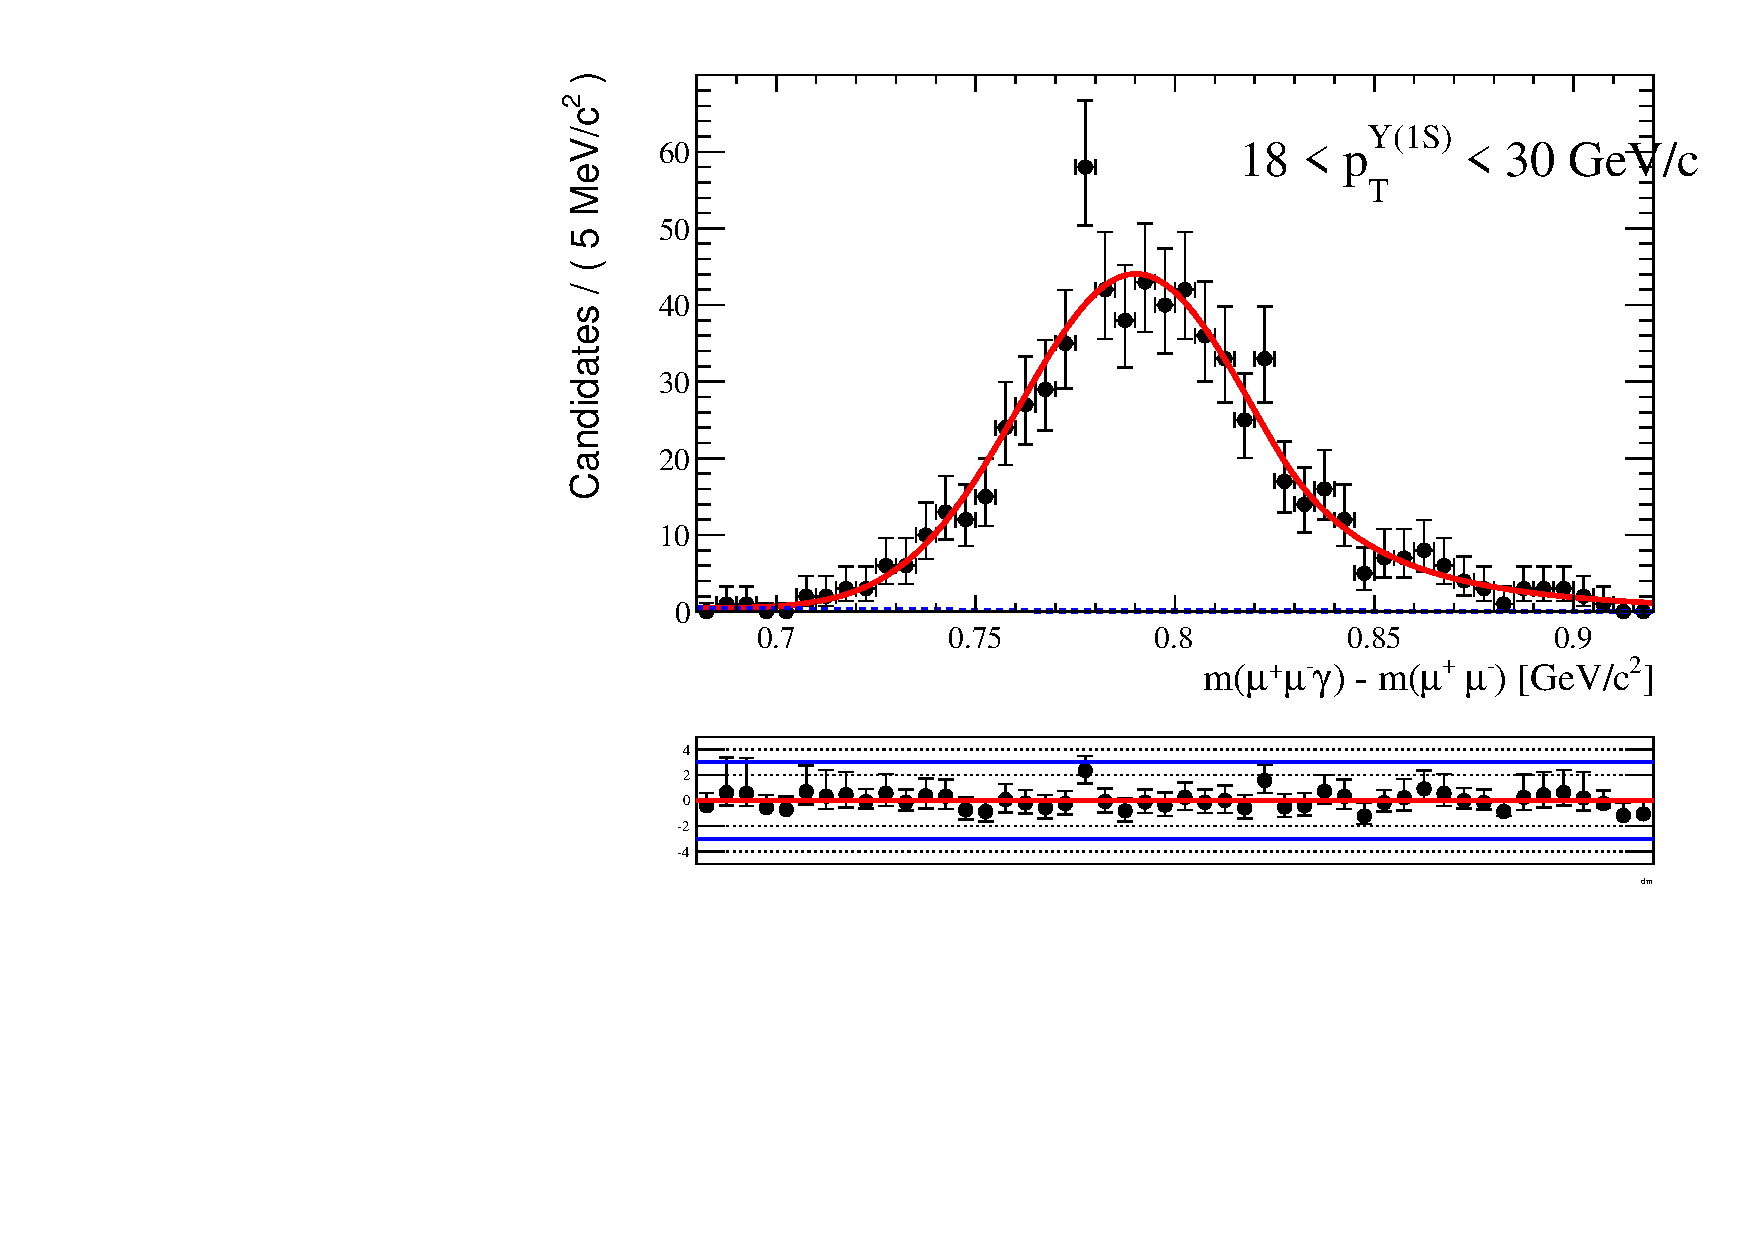
\includegraphics[width=0.16\linewidth]{fit_mc/chib12_18_30}
      \caption{\chiboneTwoP}
      \label{fig:fit_mc_chiboneTwoP}
    \end{subfigure}
    \begin{subfigure}[b]{\textwidth}
      \centering
      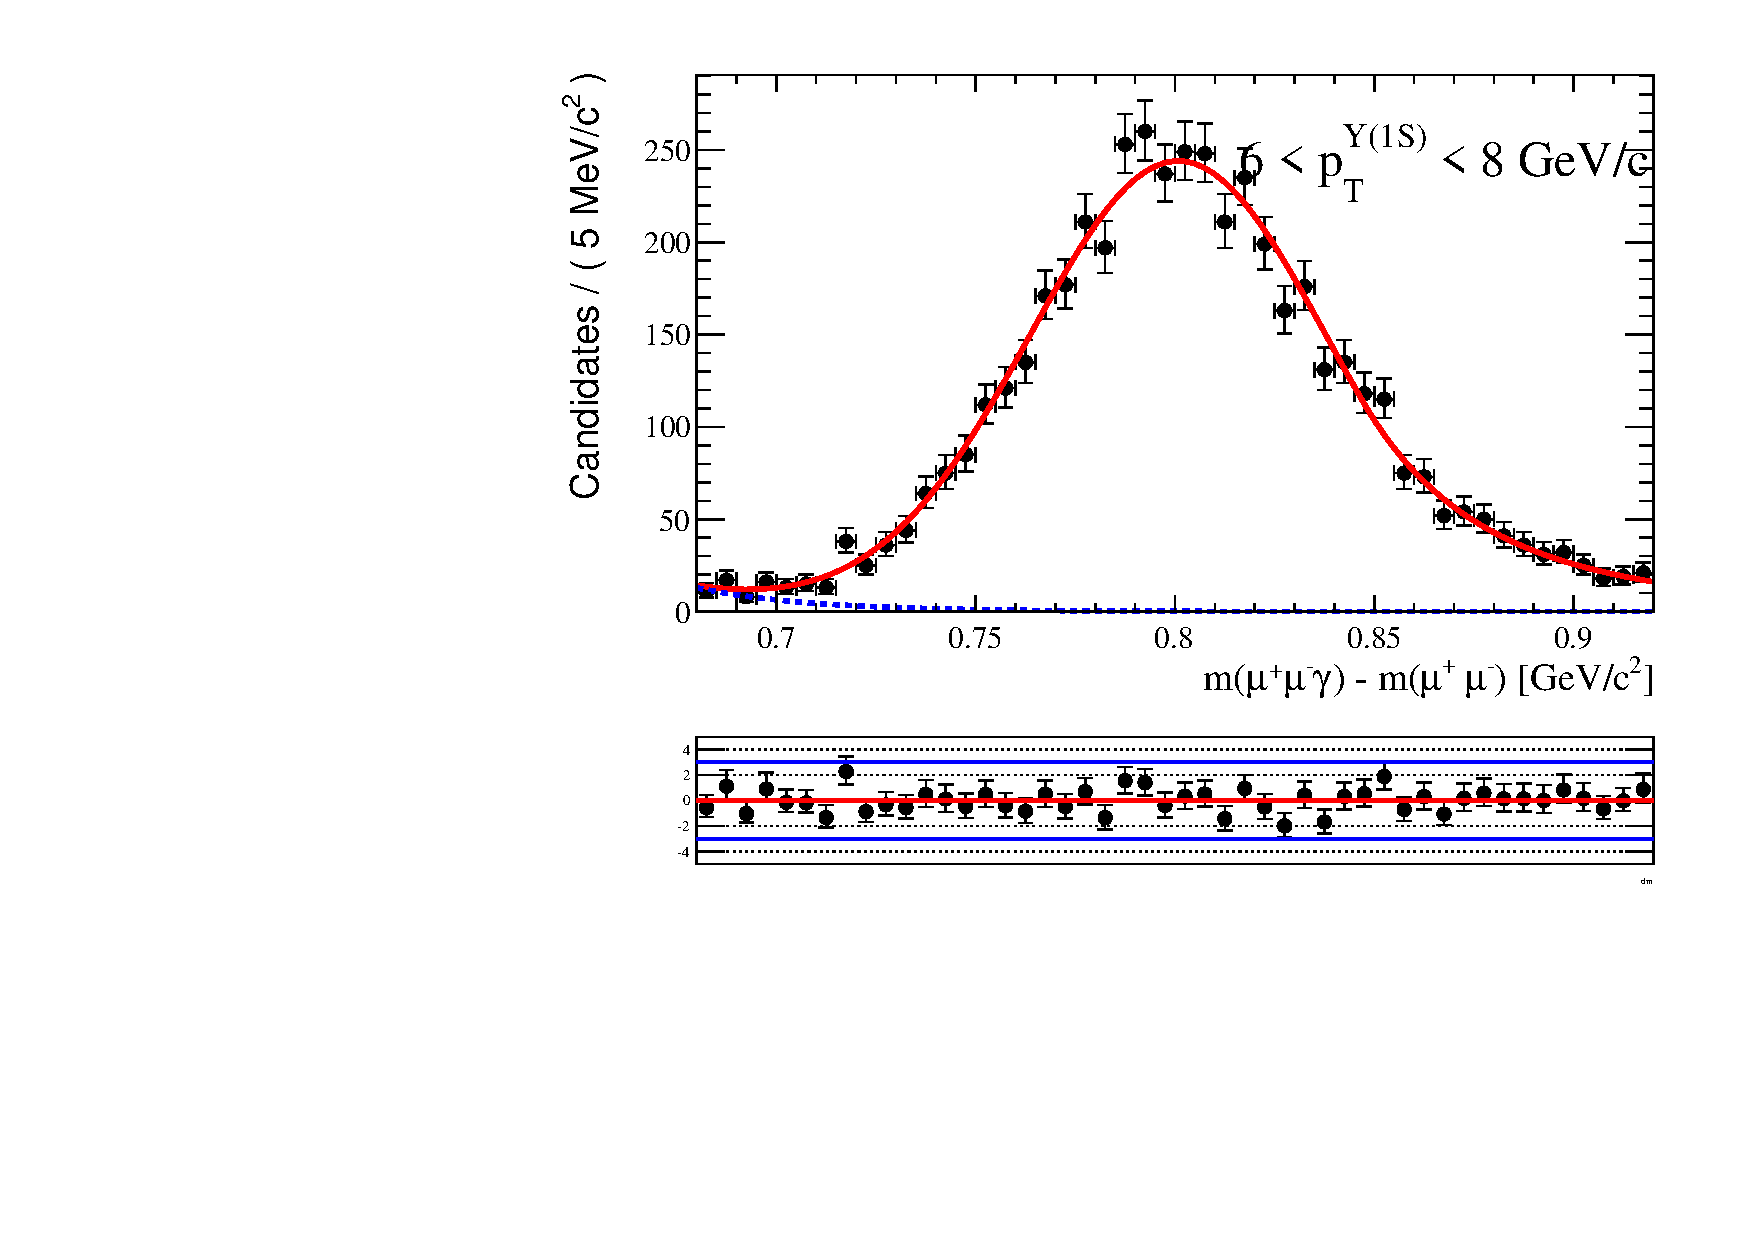
\includegraphics[width=0.16\linewidth]{fit_mc/chib22_6_8}
      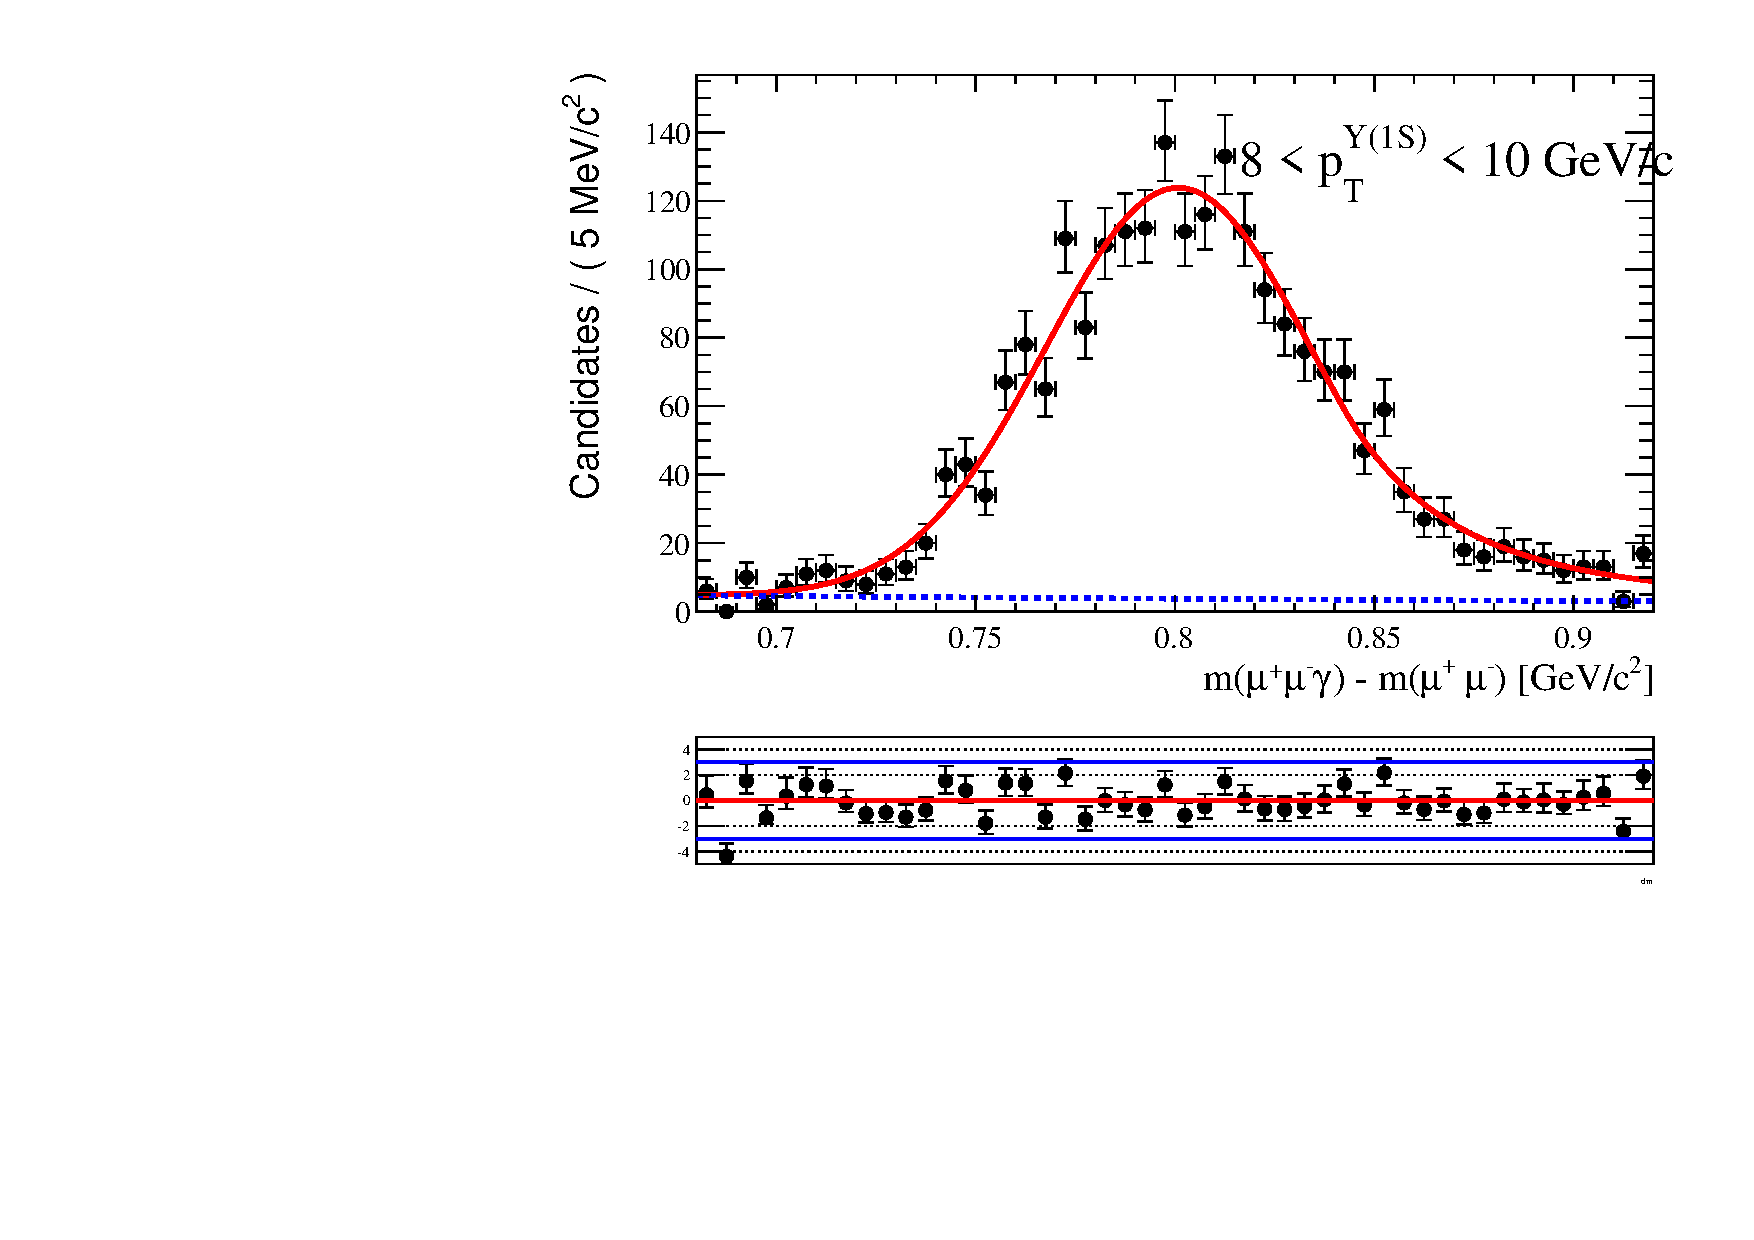
\includegraphics[width=0.16\linewidth]{fit_mc/chib22_8_10}
      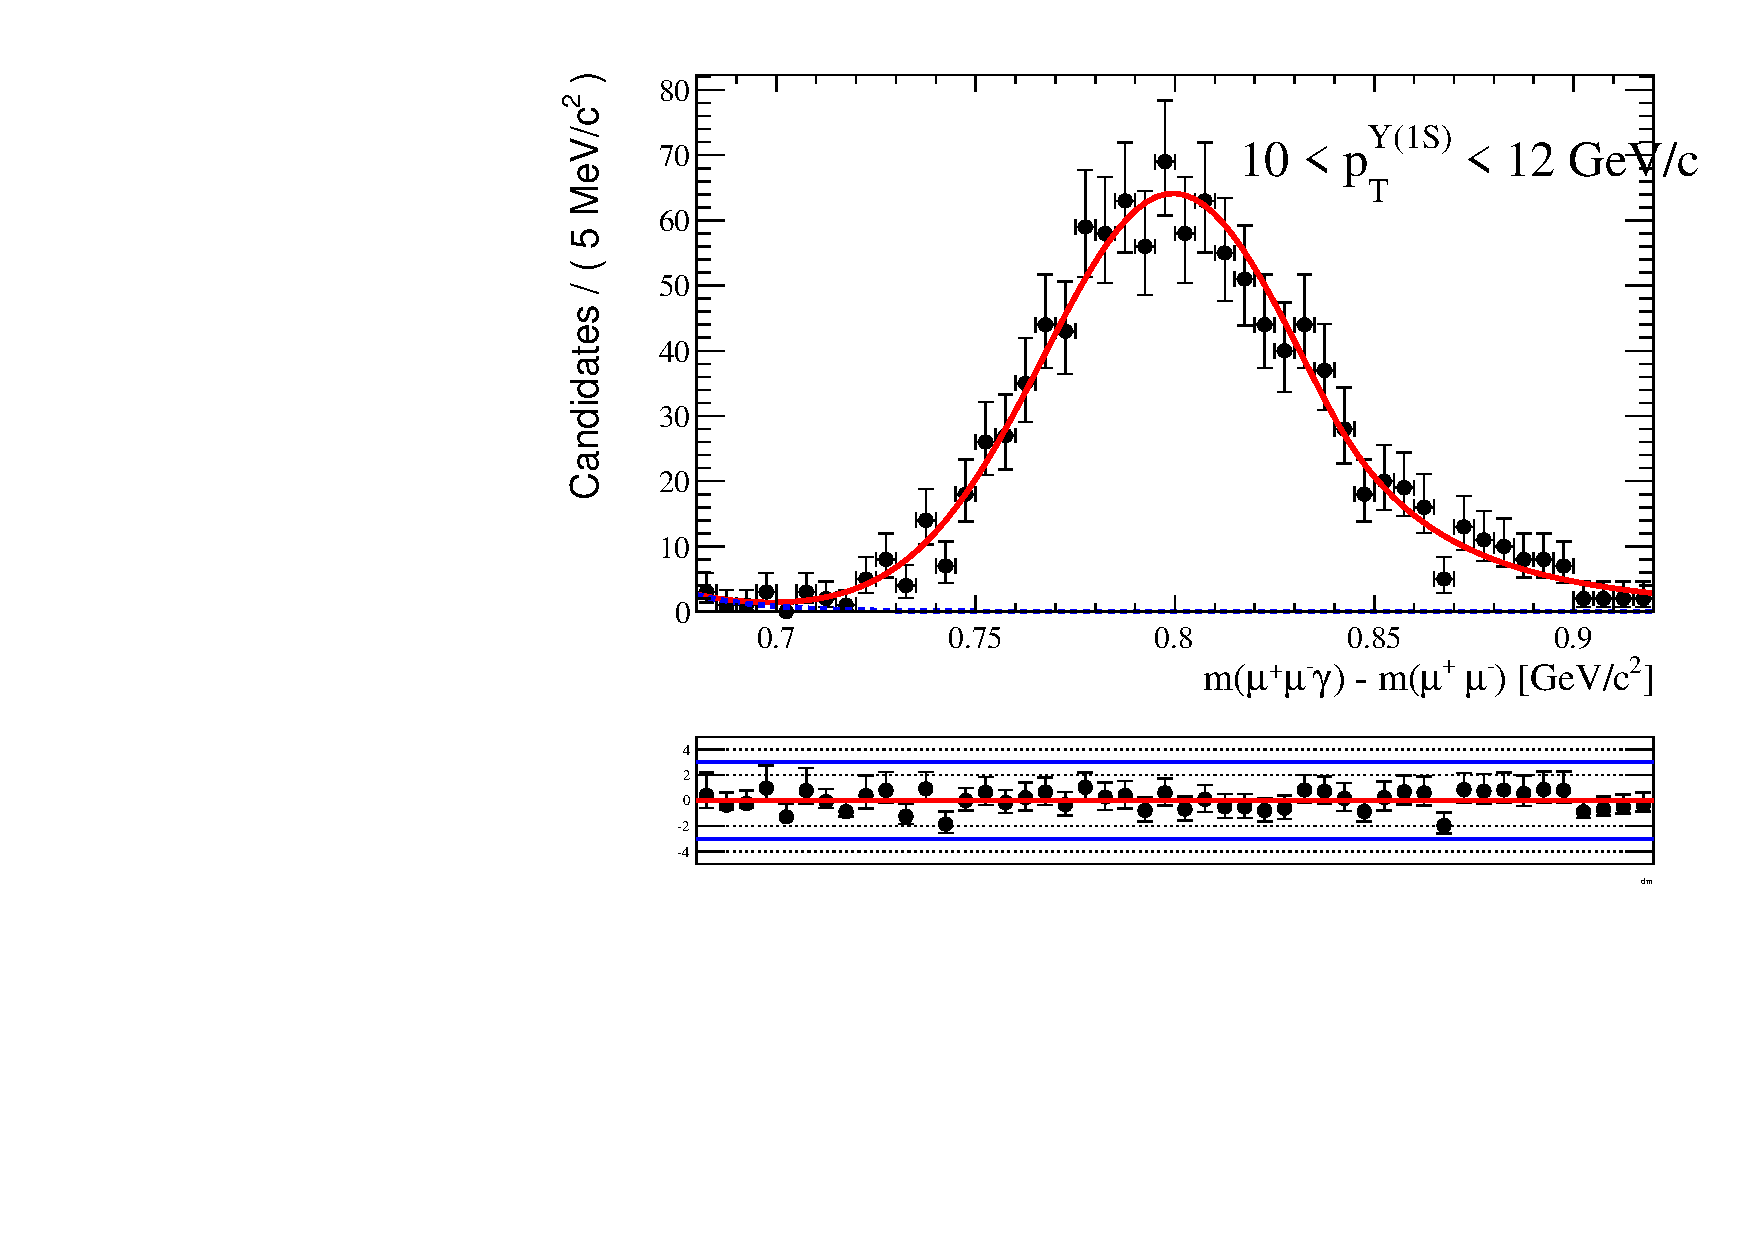
\includegraphics[width=0.16\linewidth]{fit_mc/chib22_10_12}
      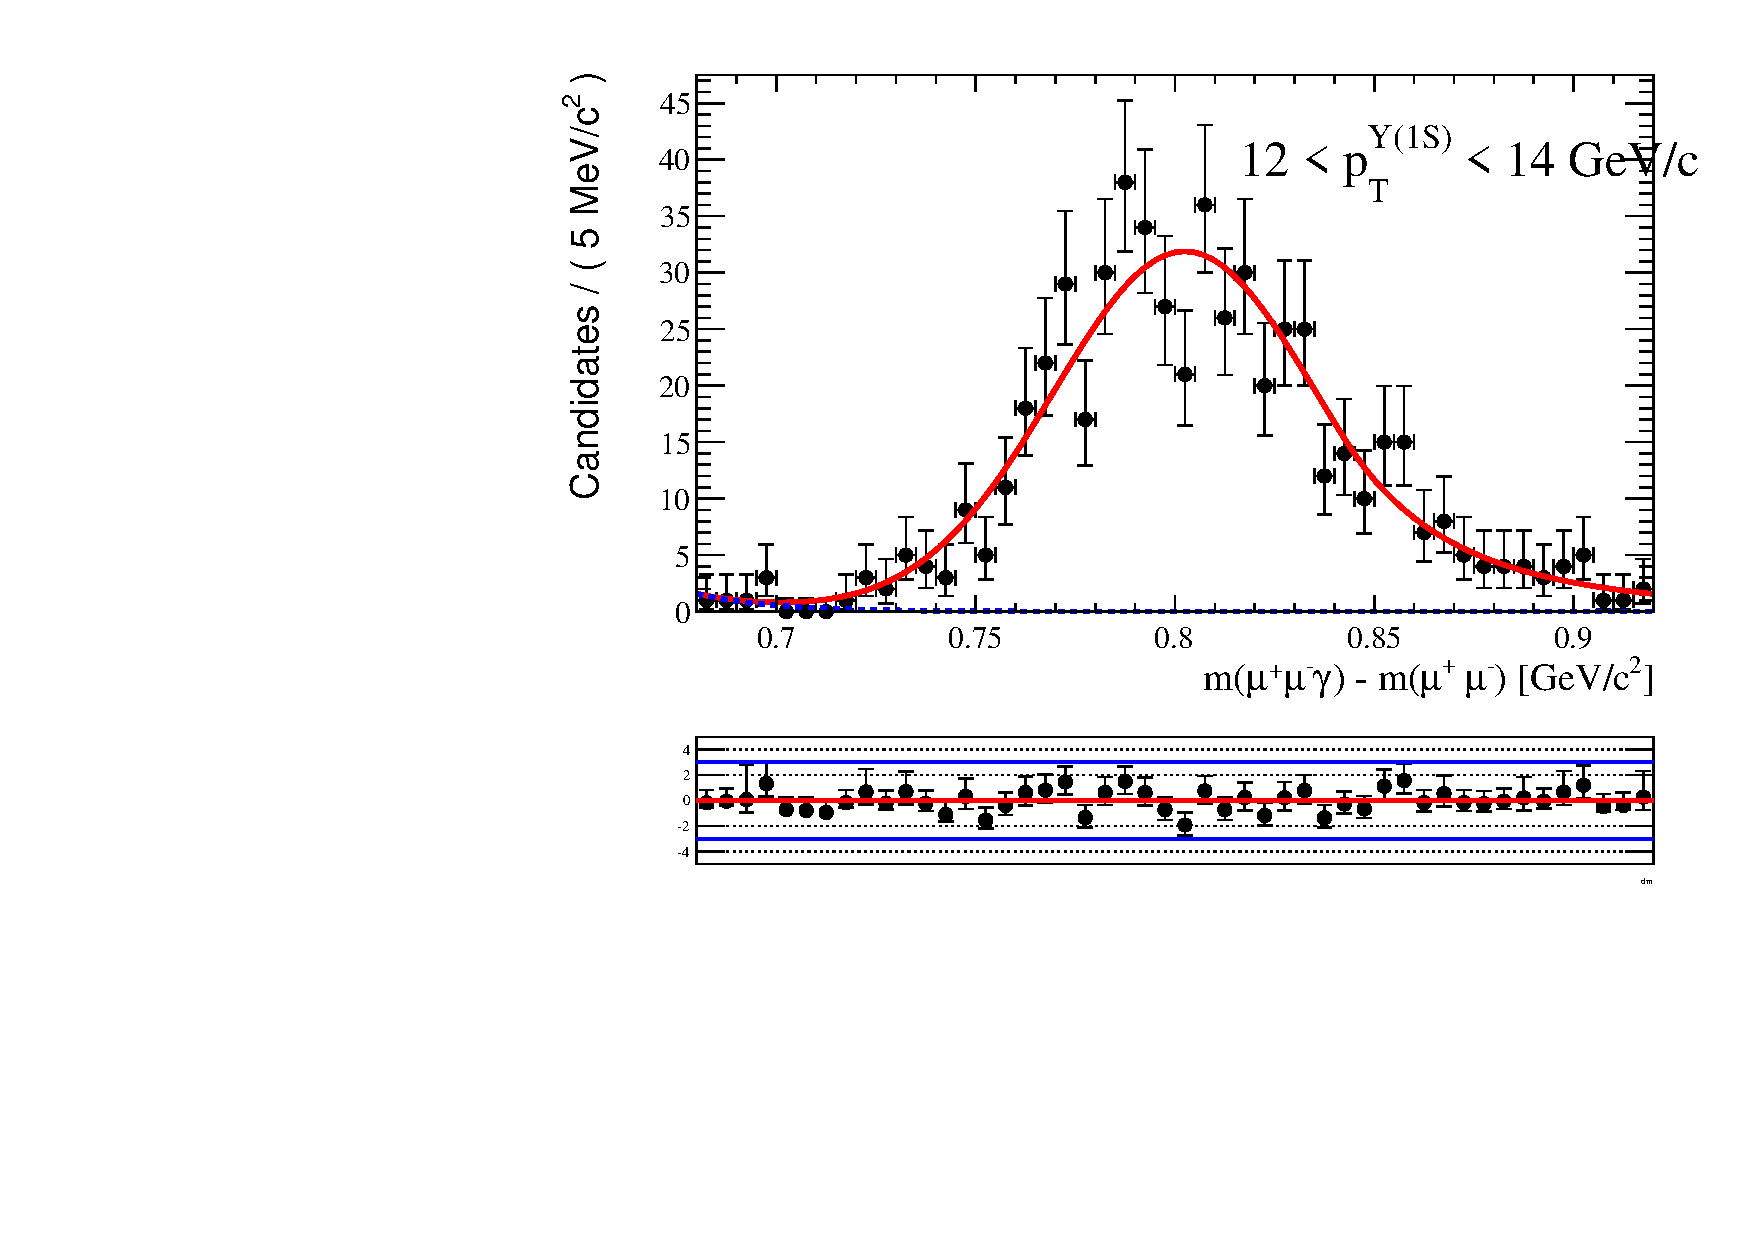
\includegraphics[width=0.16\linewidth]{fit_mc/chib22_12_14}
      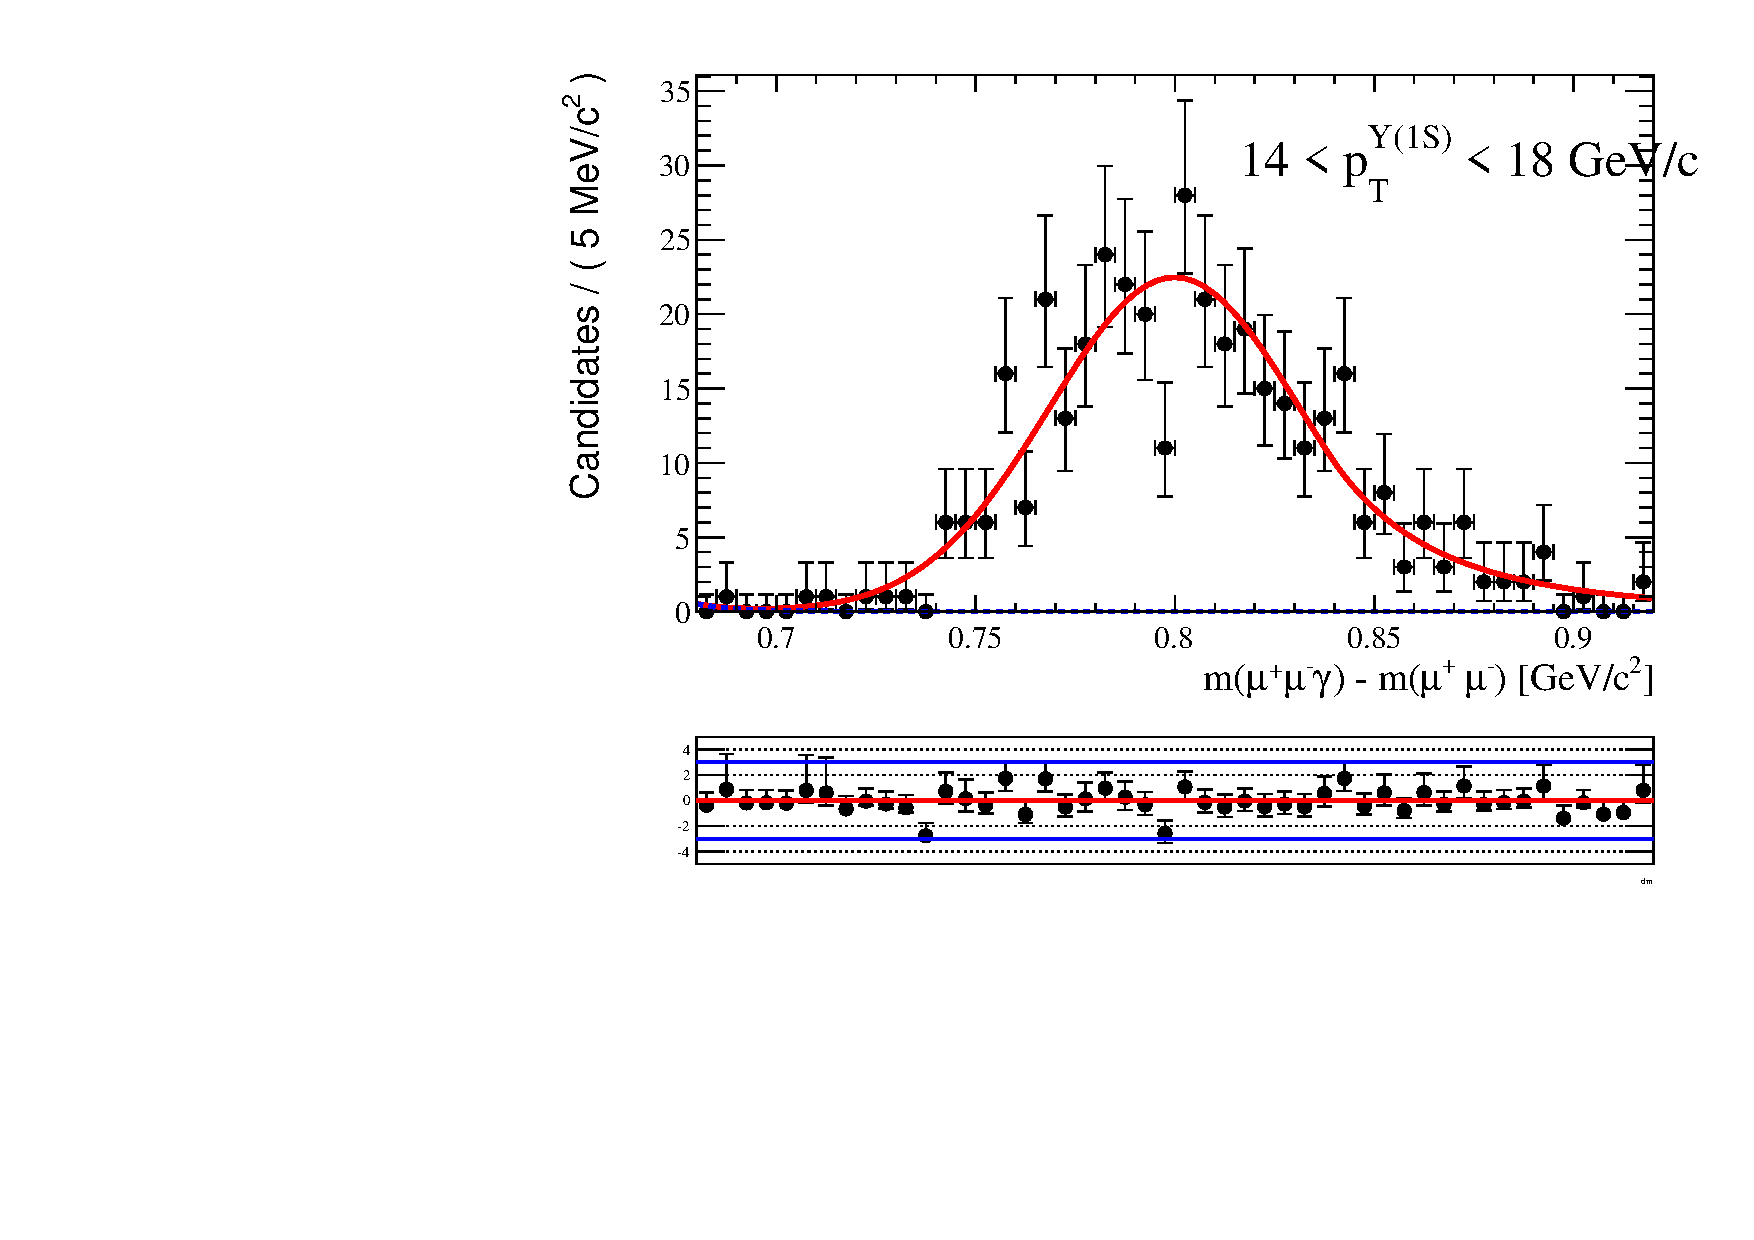
\includegraphics[width=0.16\linewidth]{fit_mc/chib22_14_18}
      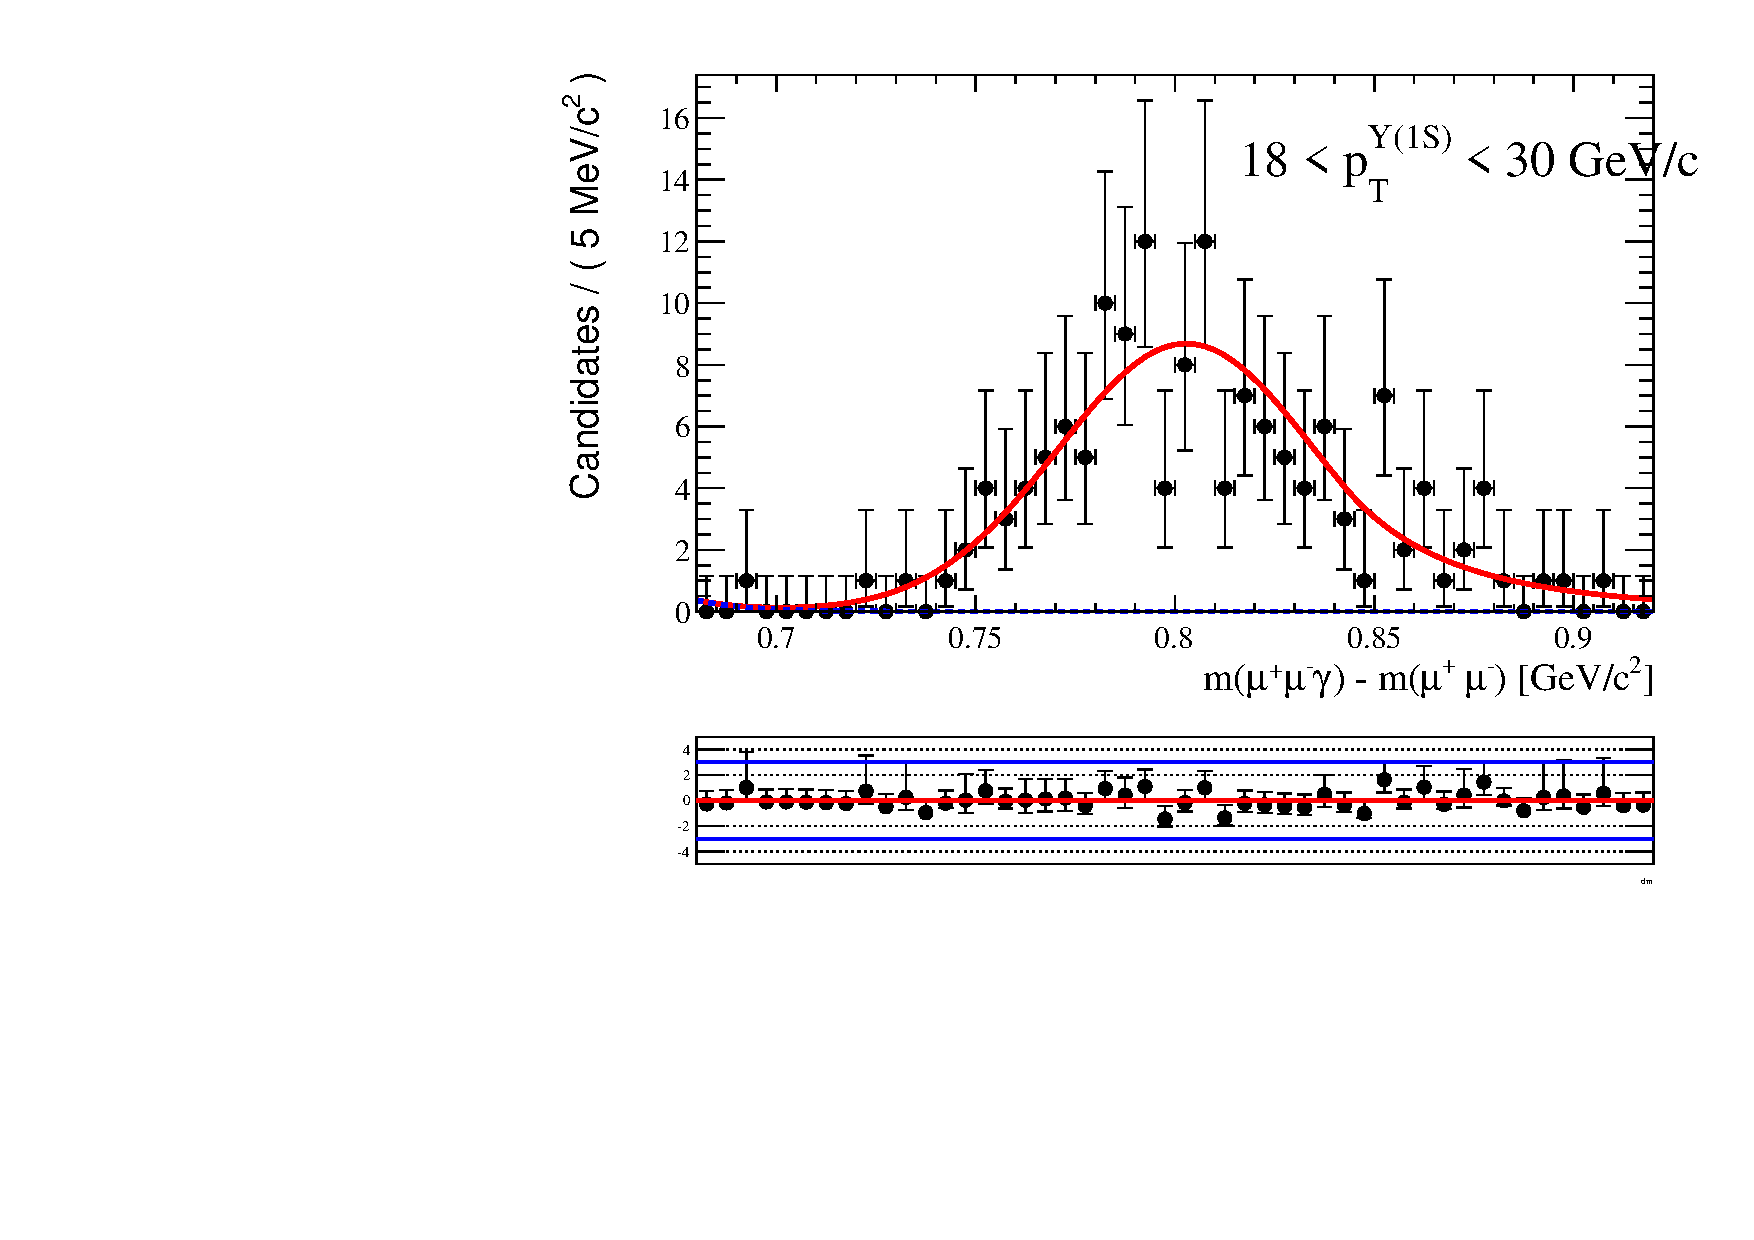
\includegraphics[width=0.16\linewidth]{fit_mc/chib22_18_30}
      \caption{\chibtwoTwoP}
      \label{fig:fit_mc_chibtwoTwoP}
    \end{subfigure}    
    \begin{subfigure}[b]{\textwidth}
      \centering
      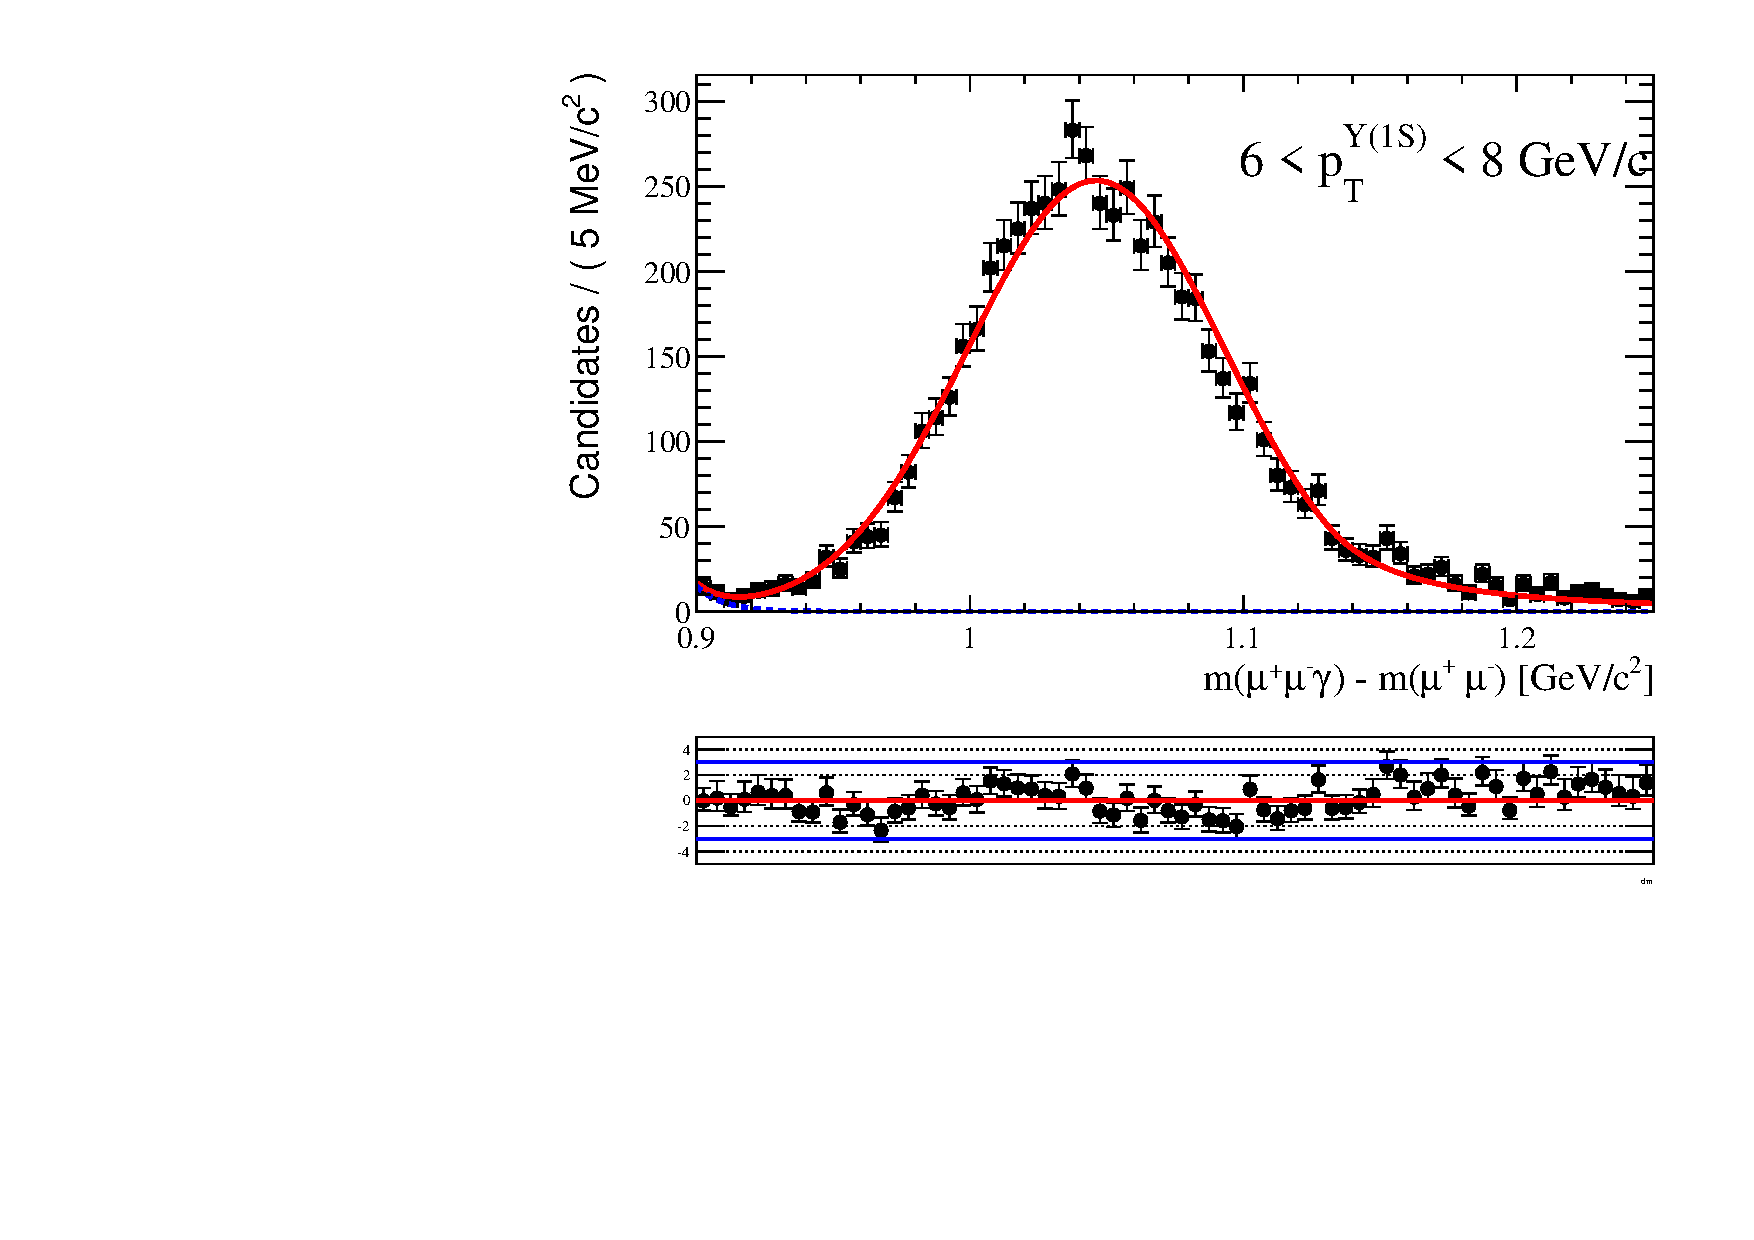
\includegraphics[width=0.16\linewidth]{fit_mc/chib13_6_8}
      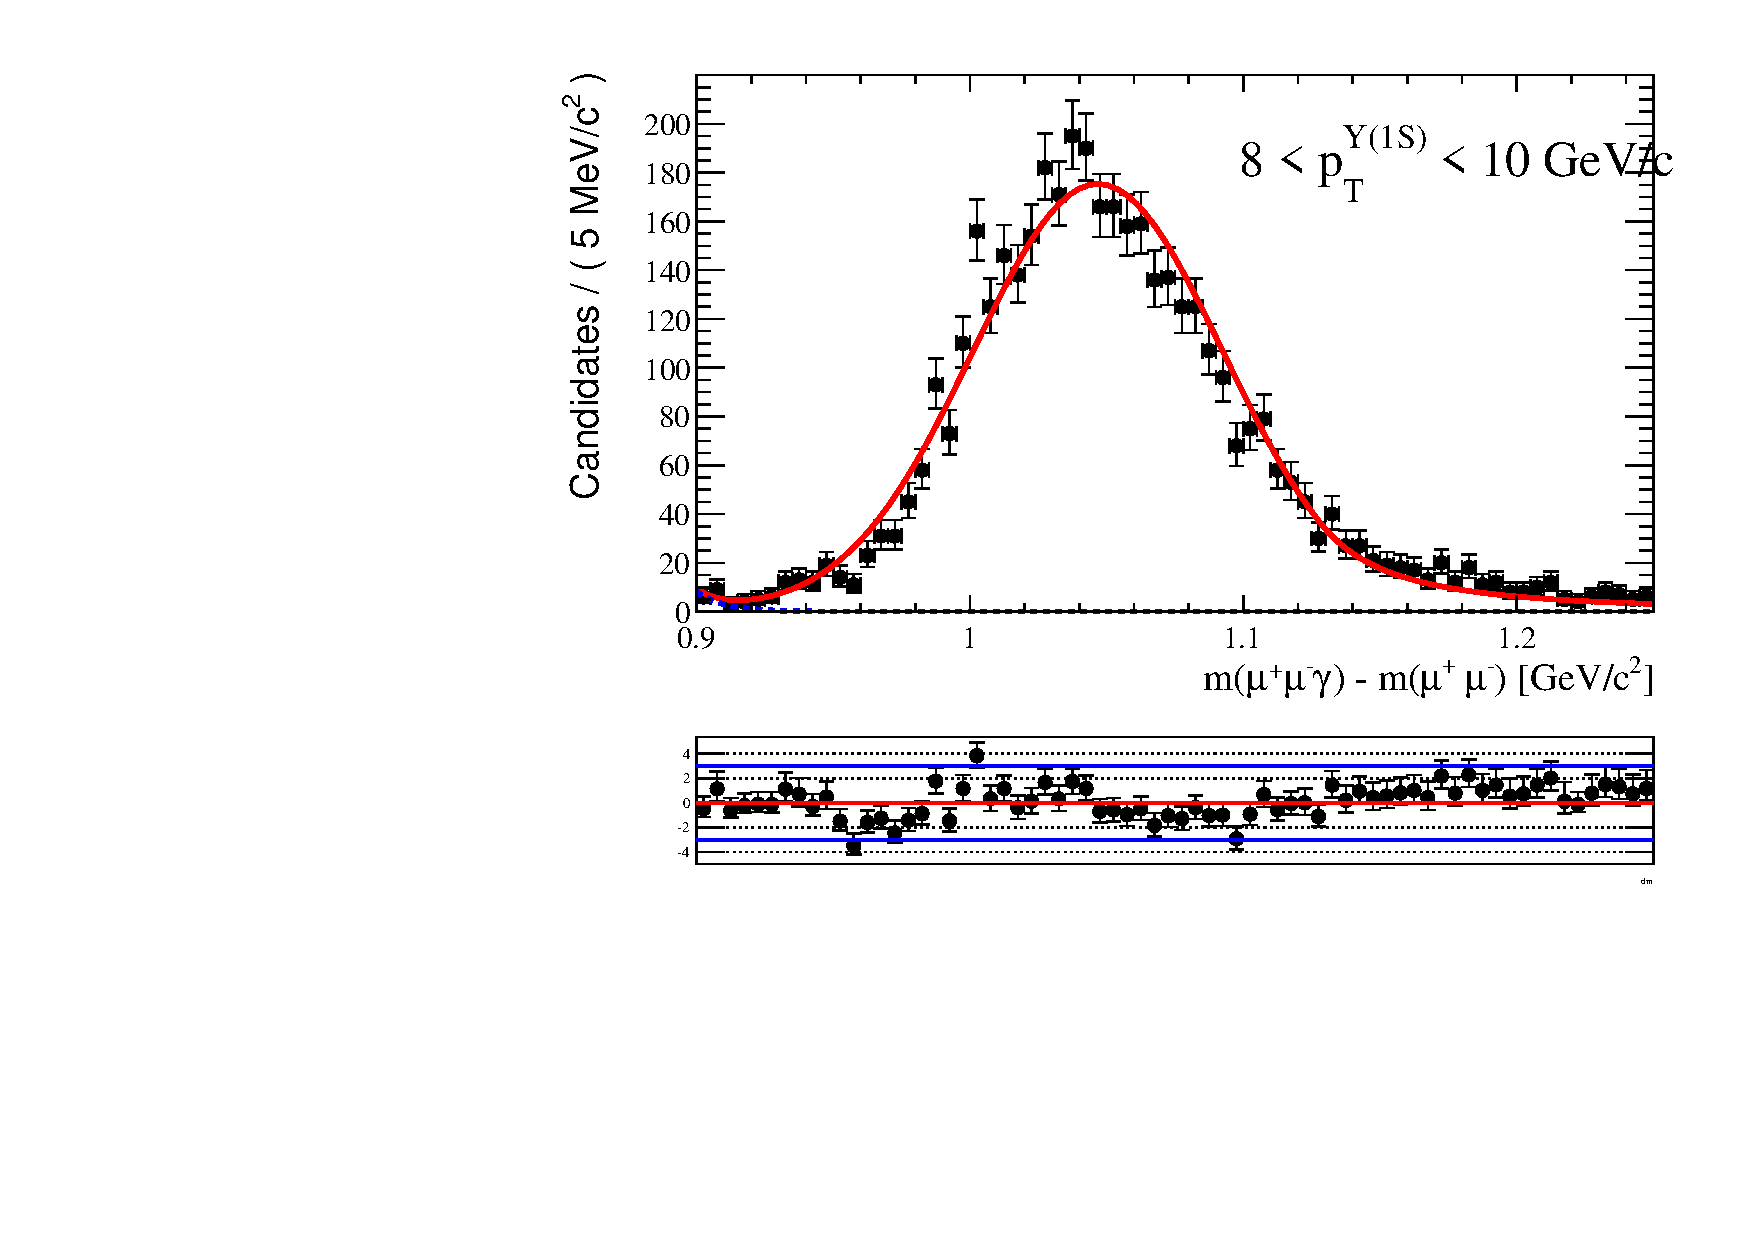
\includegraphics[width=0.16\linewidth]{fit_mc/chib13_8_10}
      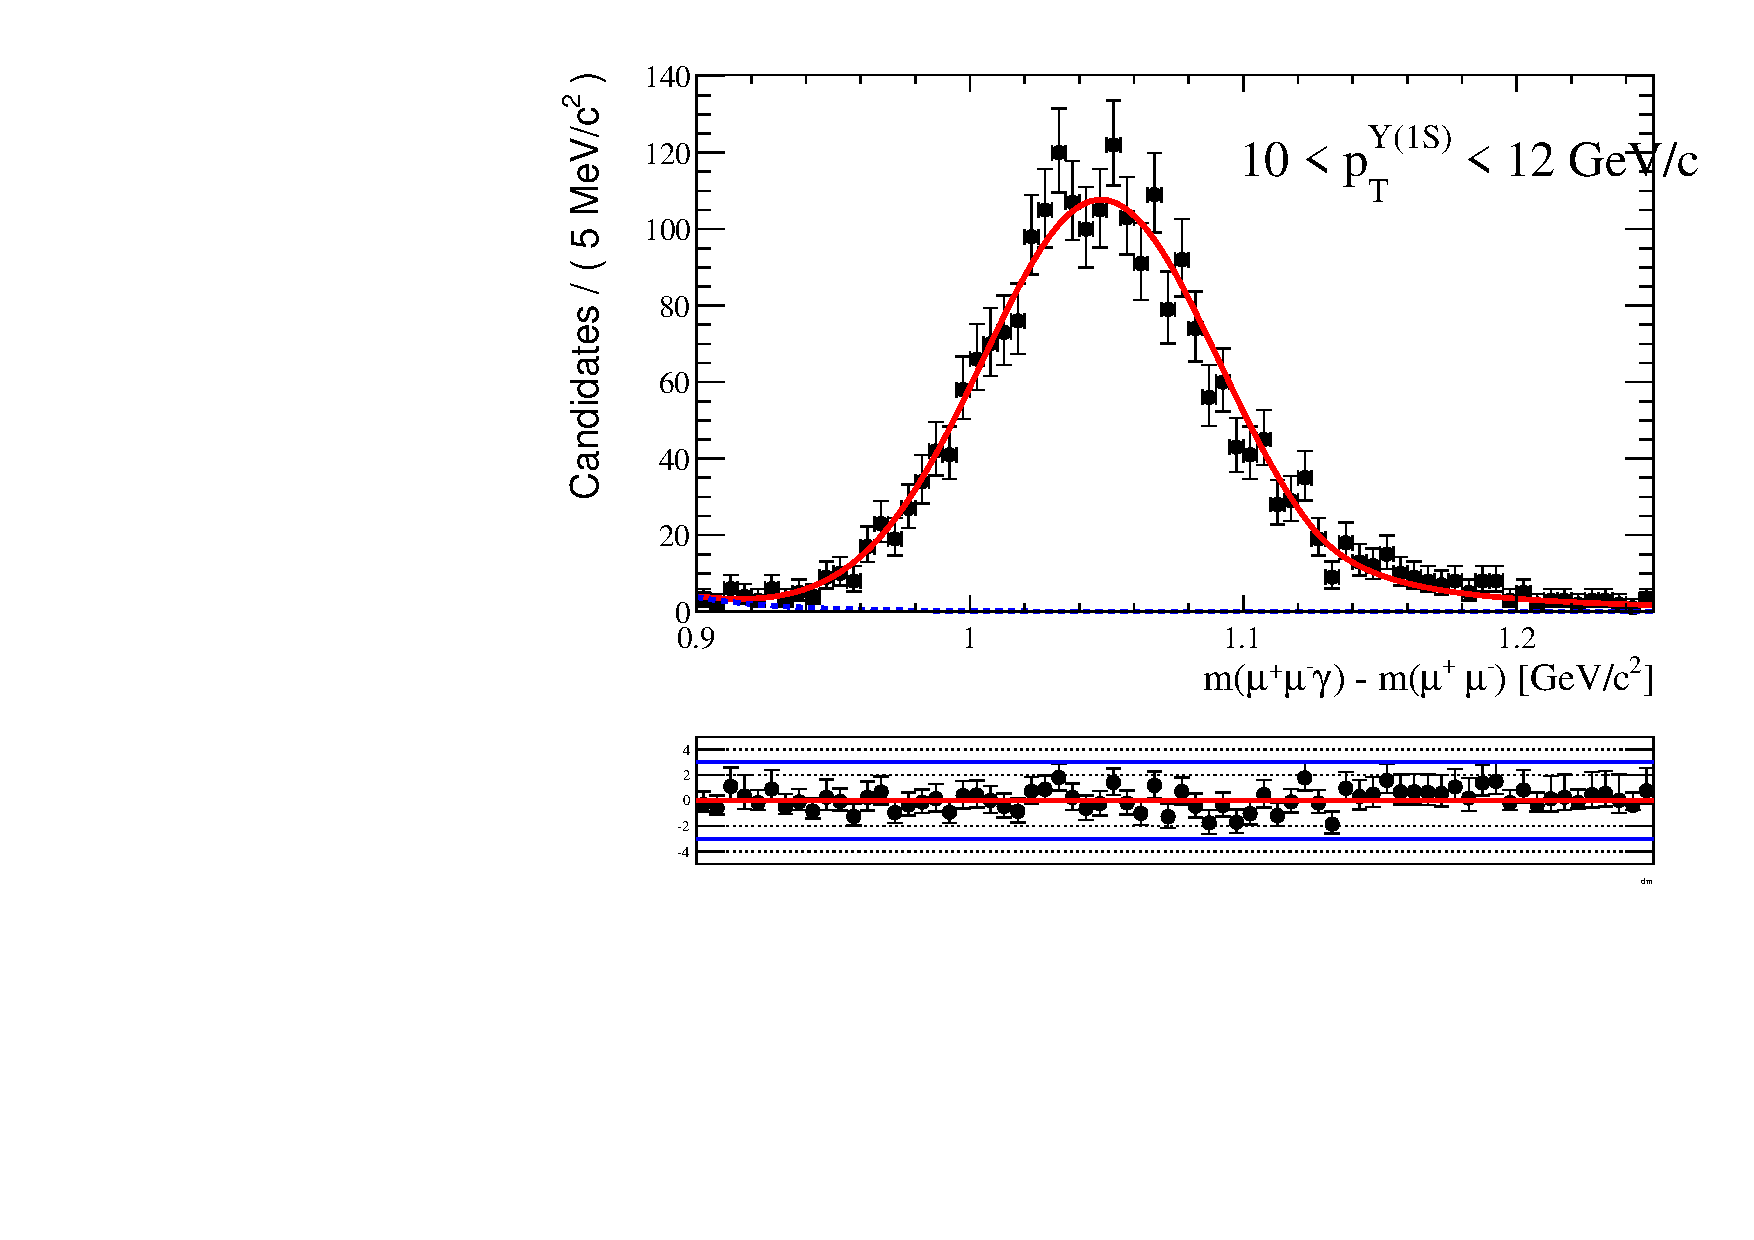
\includegraphics[width=0.16\linewidth]{fit_mc/chib13_10_12}
      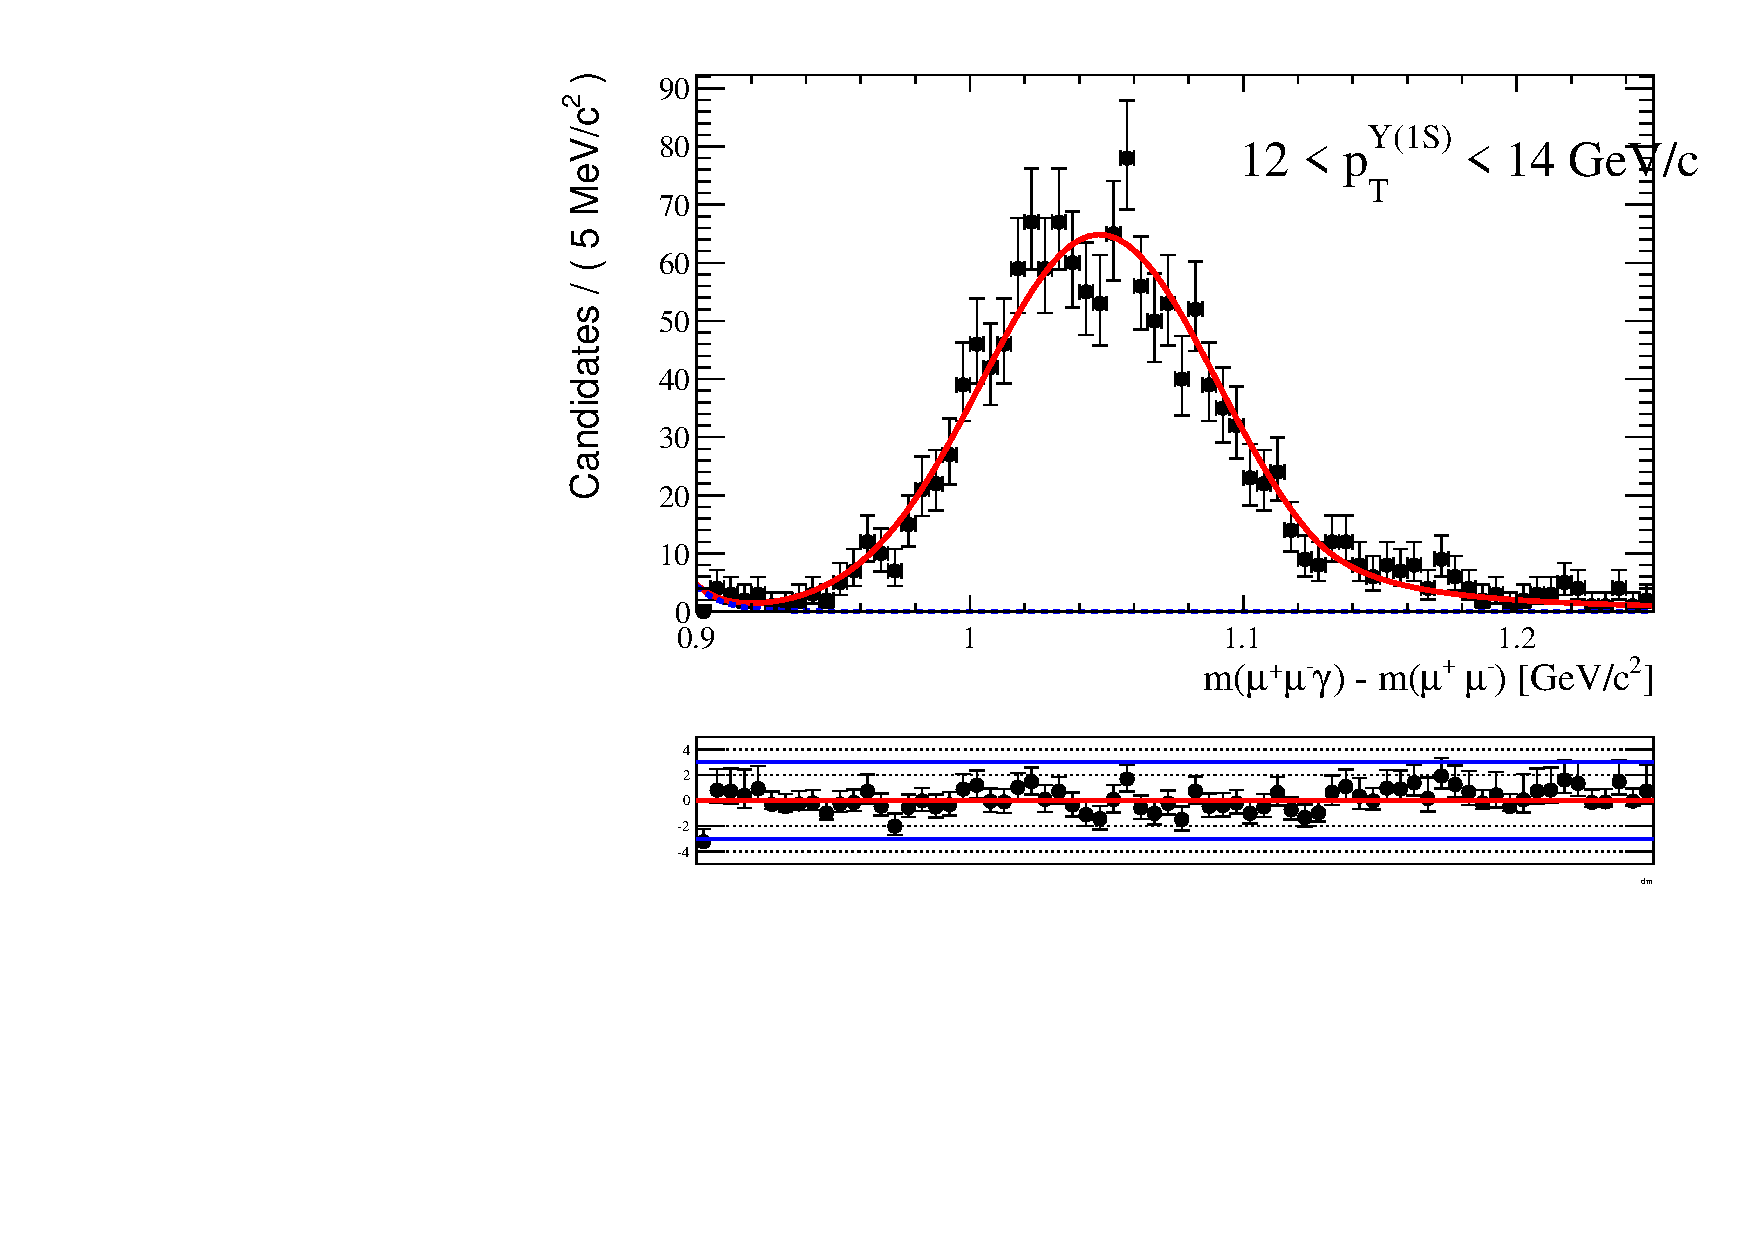
\includegraphics[width=0.16\linewidth]{fit_mc/chib13_12_14}
      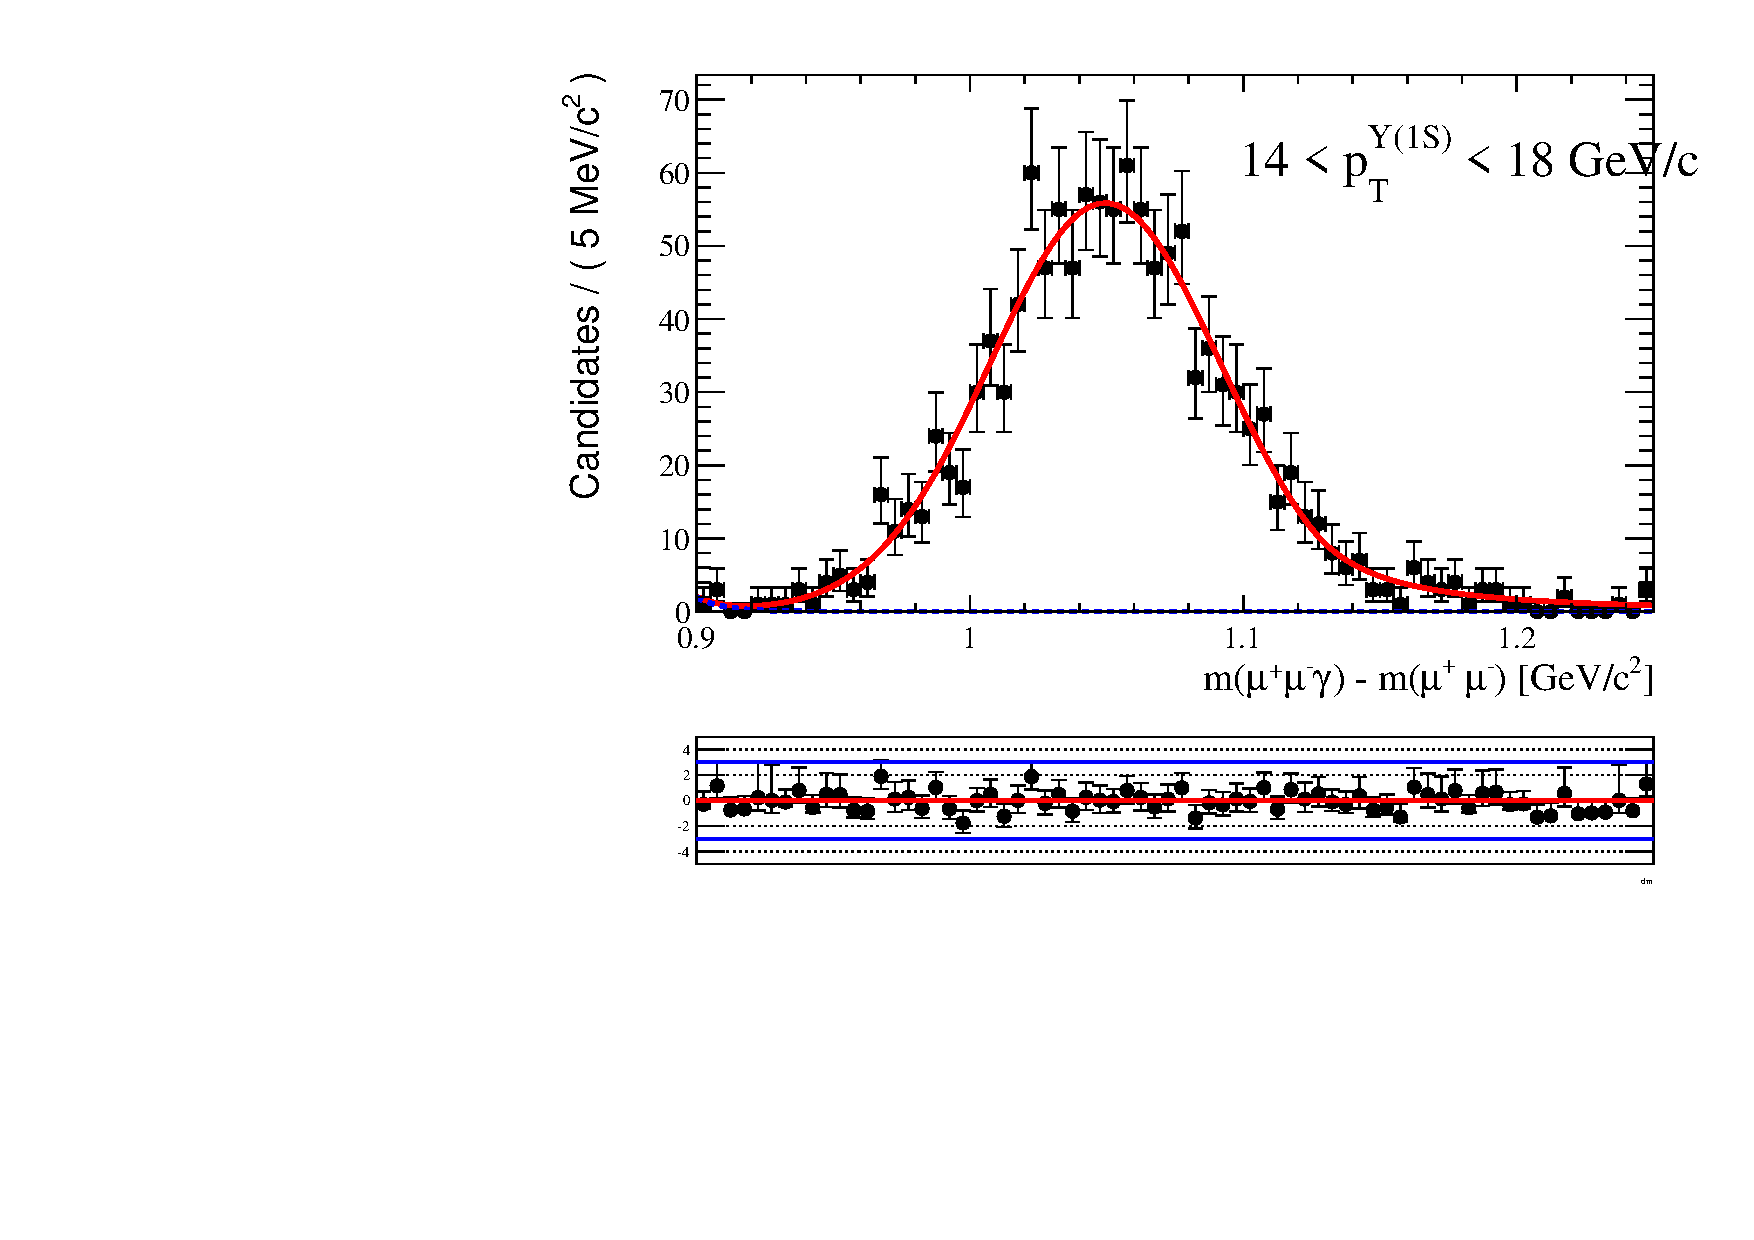
\includegraphics[width=0.16\linewidth]{fit_mc/chib13_14_18}
      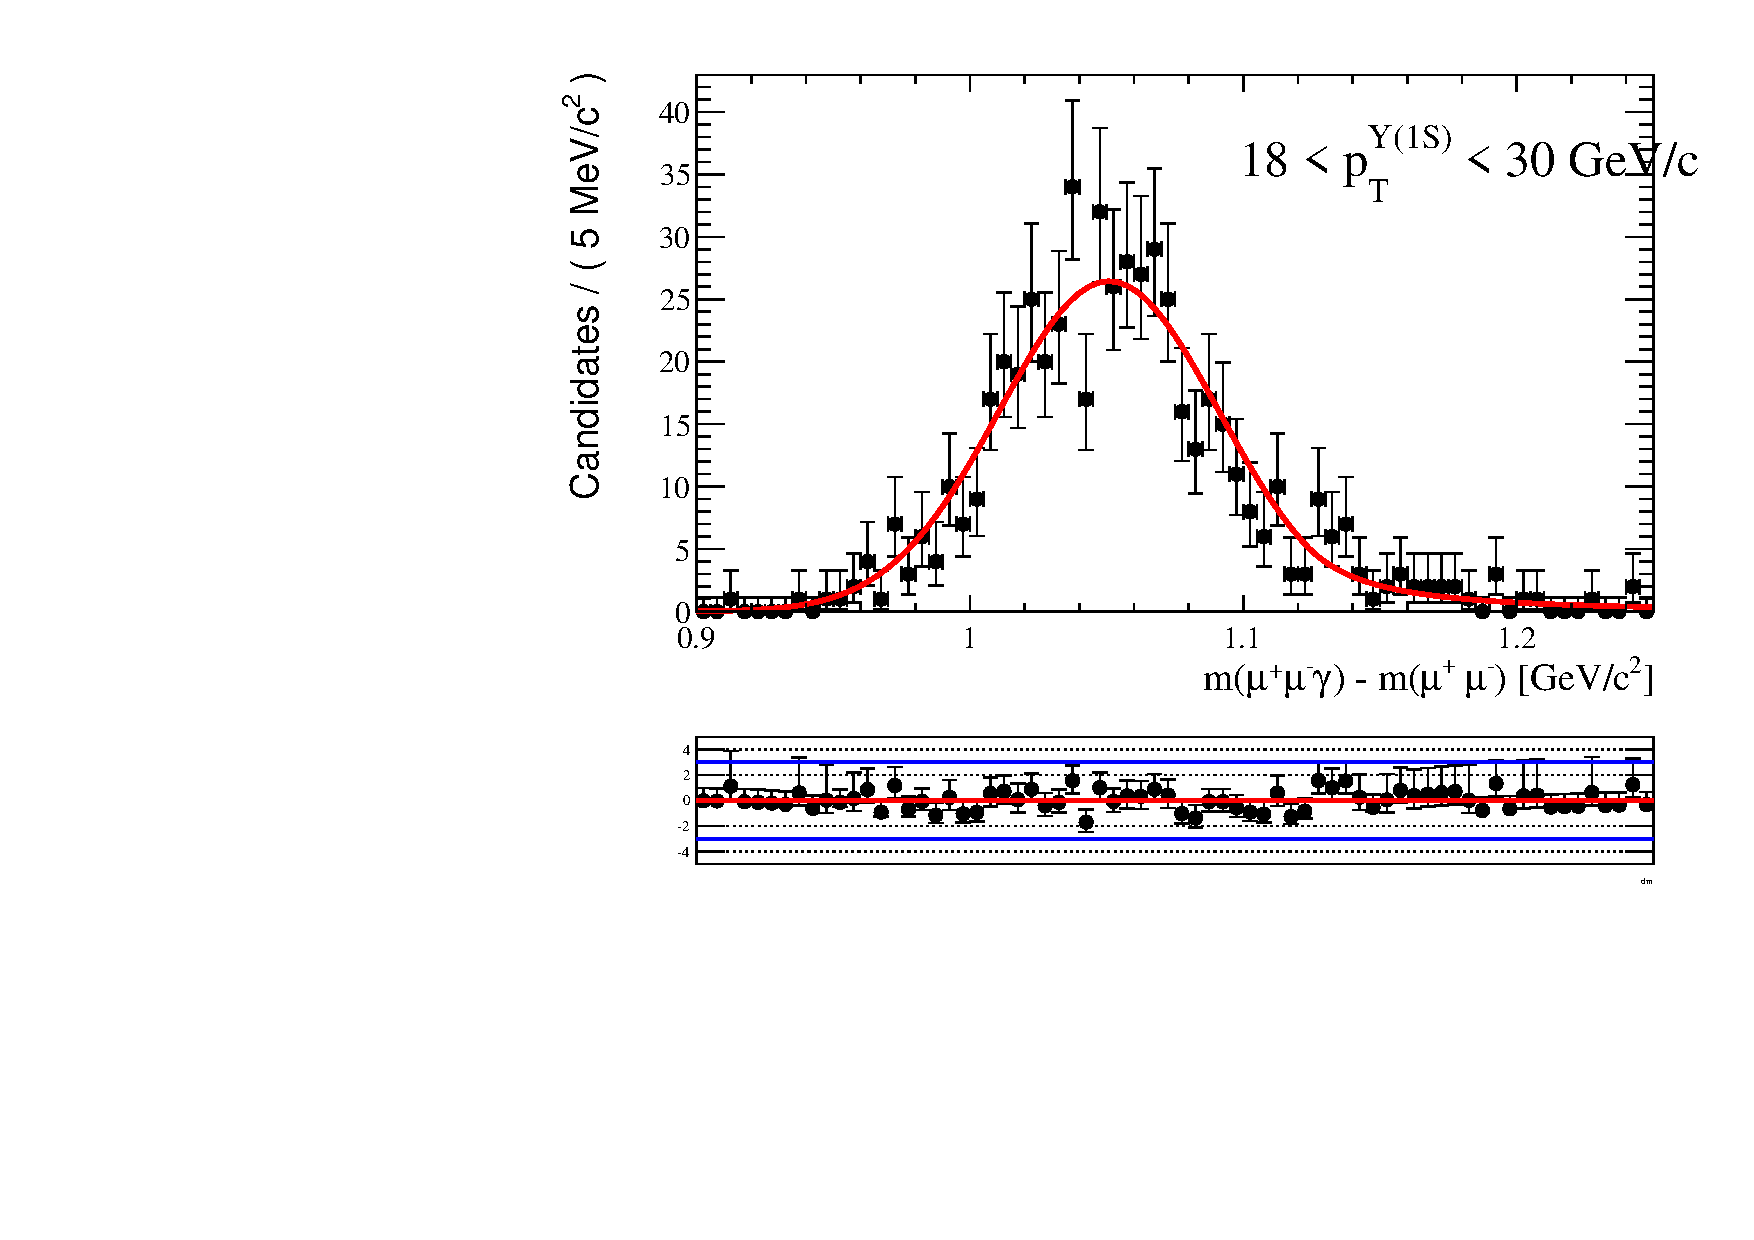
\includegraphics[width=0.16\linewidth]{fit_mc/chib13_18_30}
      \caption{\chiboneThreeP}
      \label{fig:fit_mc_chiboneThreeP}
    \end{subfigure}
    \begin{subfigure}[b]{\textwidth}
      \centering
      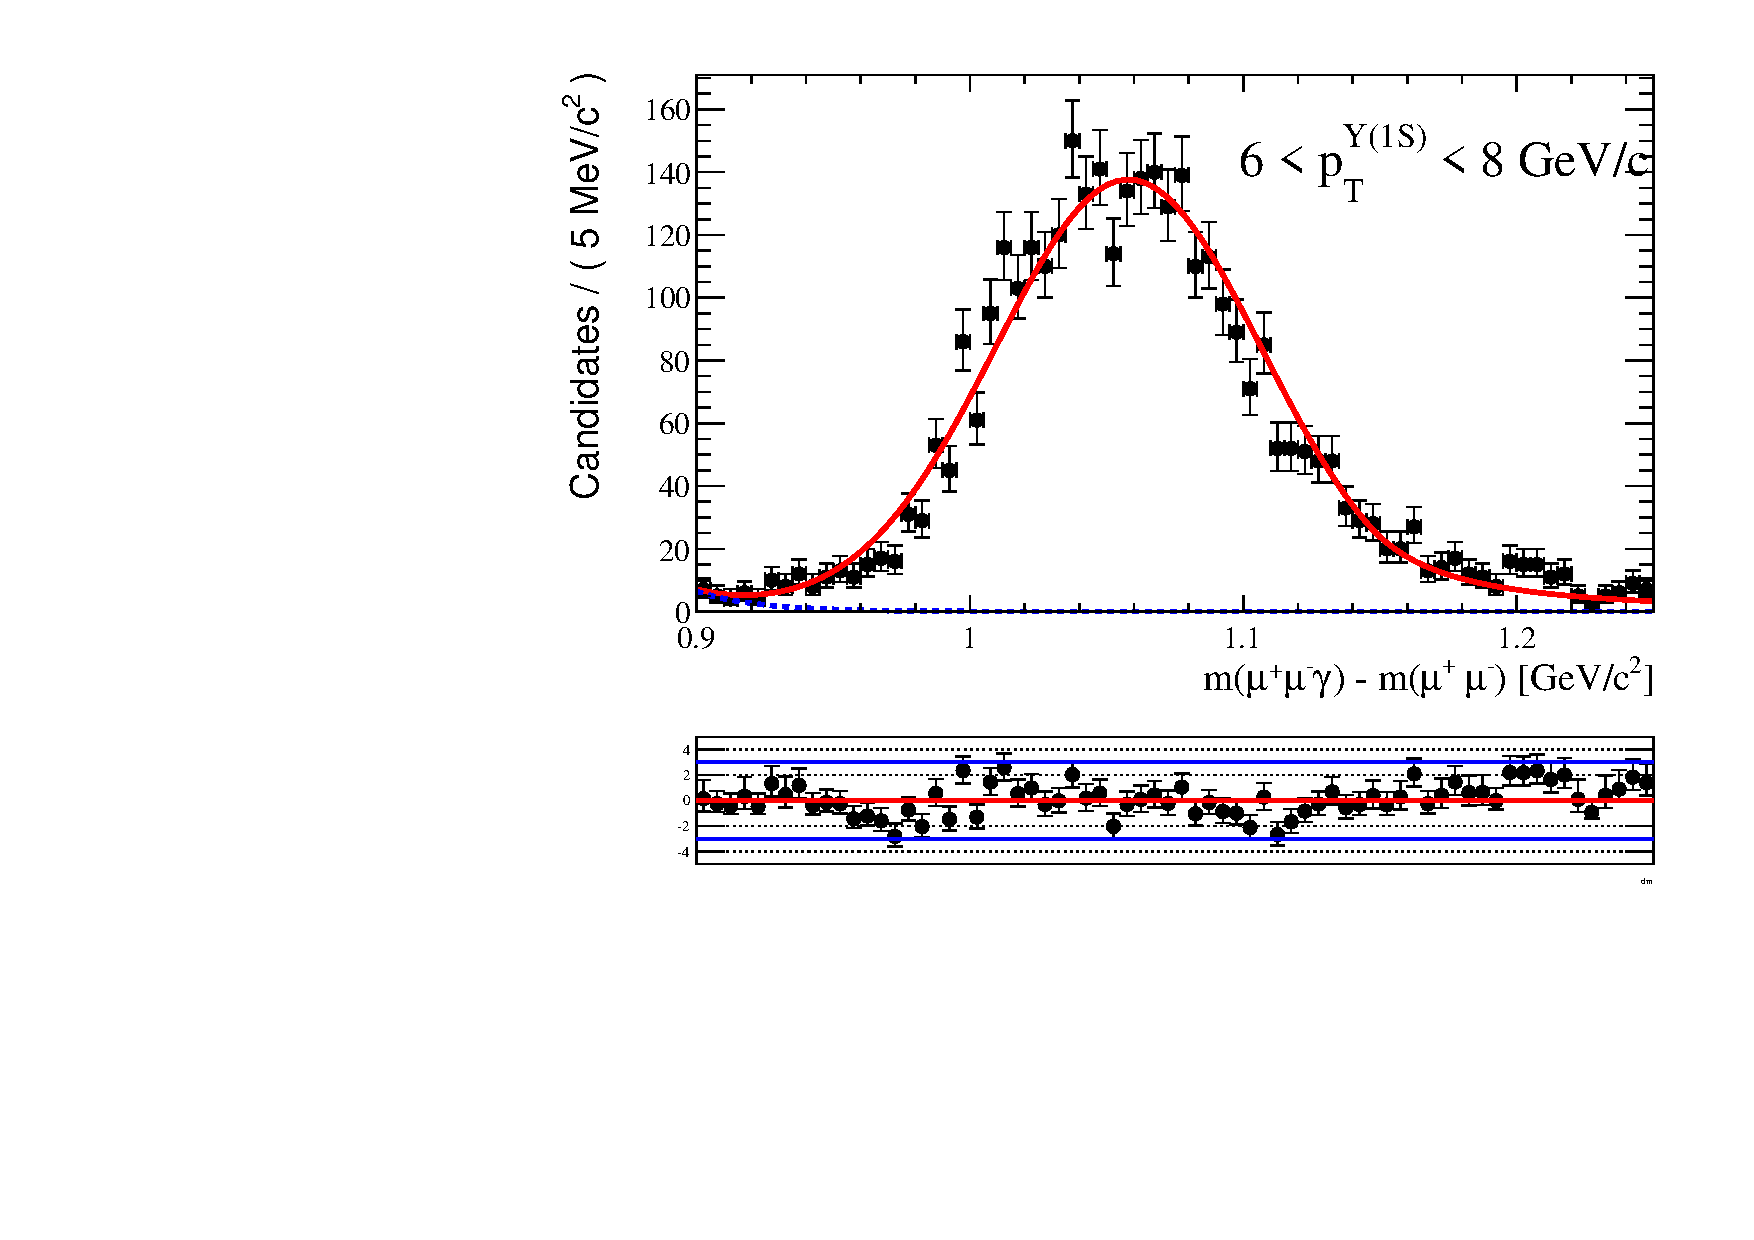
\includegraphics[width=0.16\linewidth]{fit_mc/chib23_6_8}
      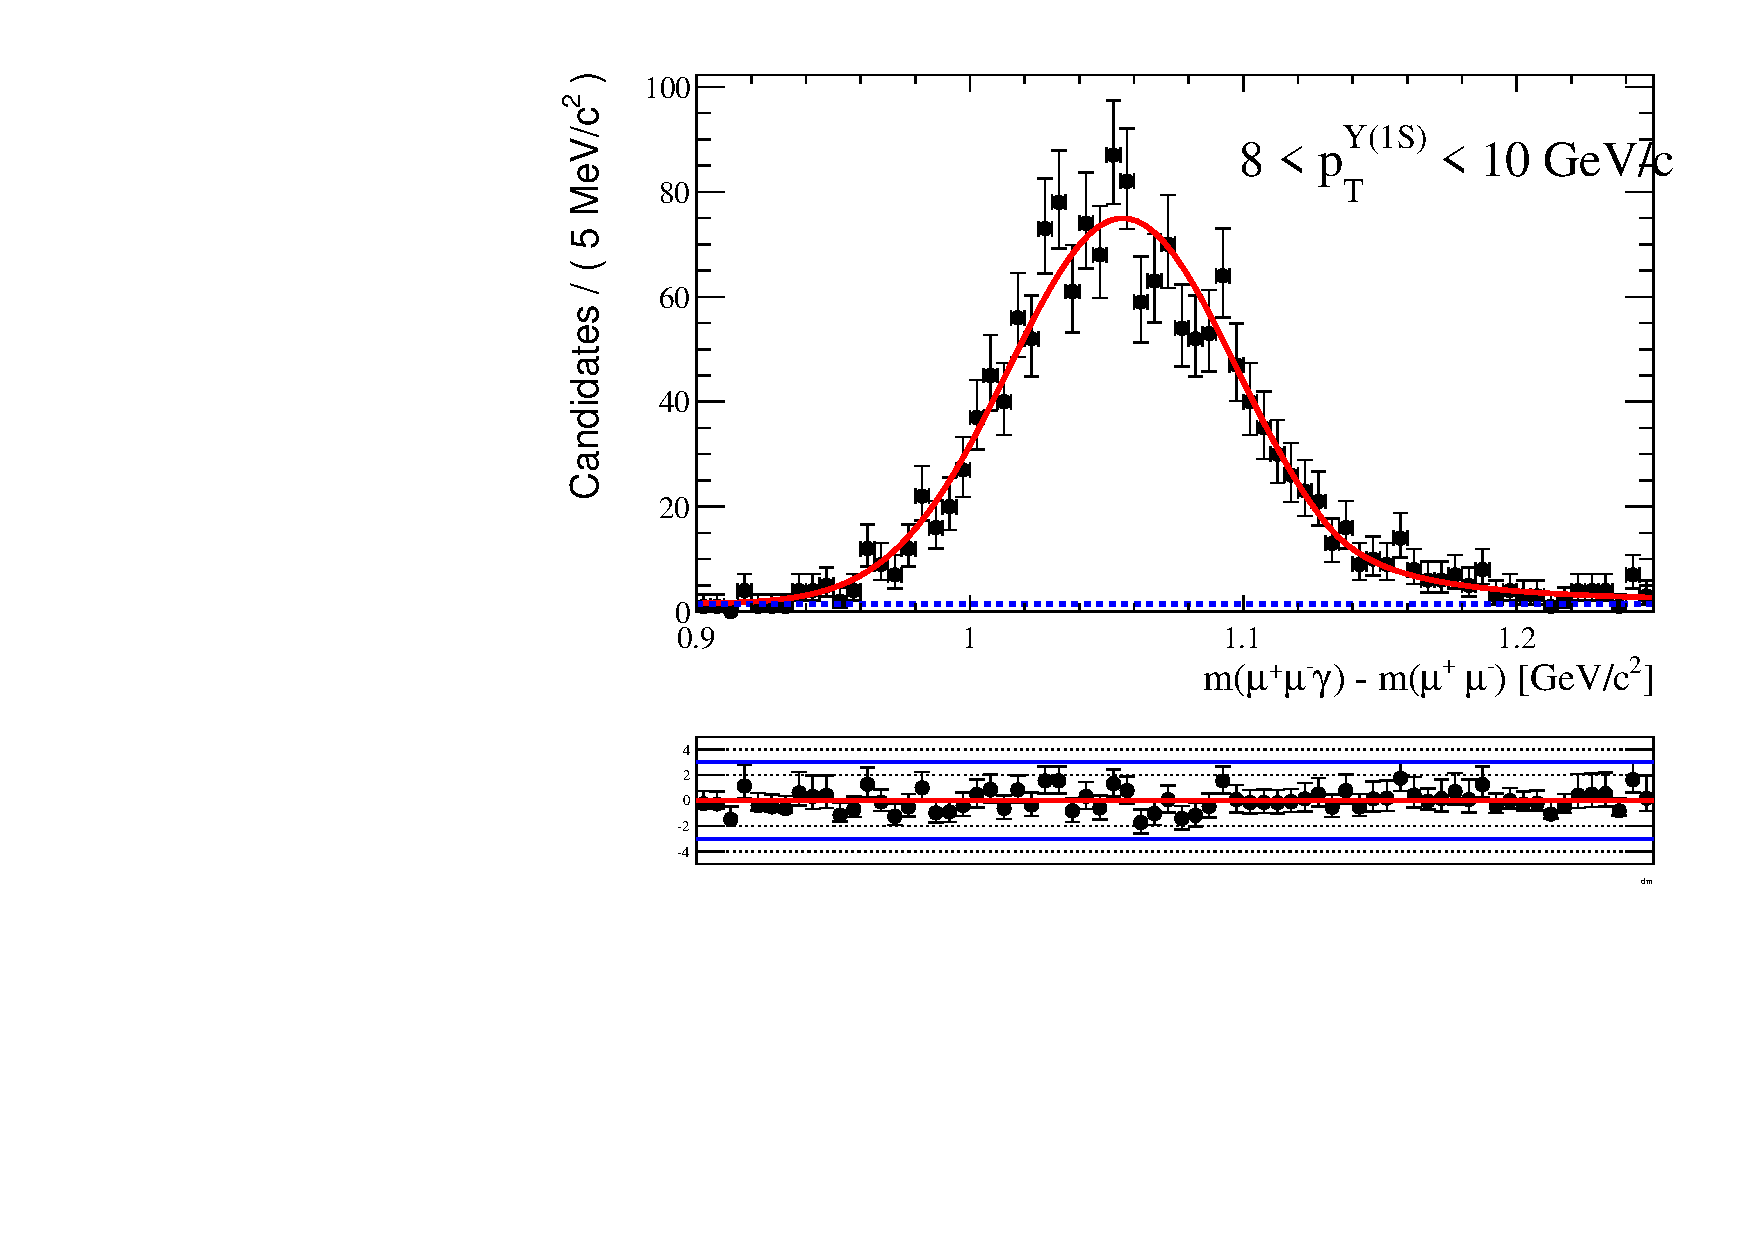
\includegraphics[width=0.16\linewidth]{fit_mc/chib23_8_10}
      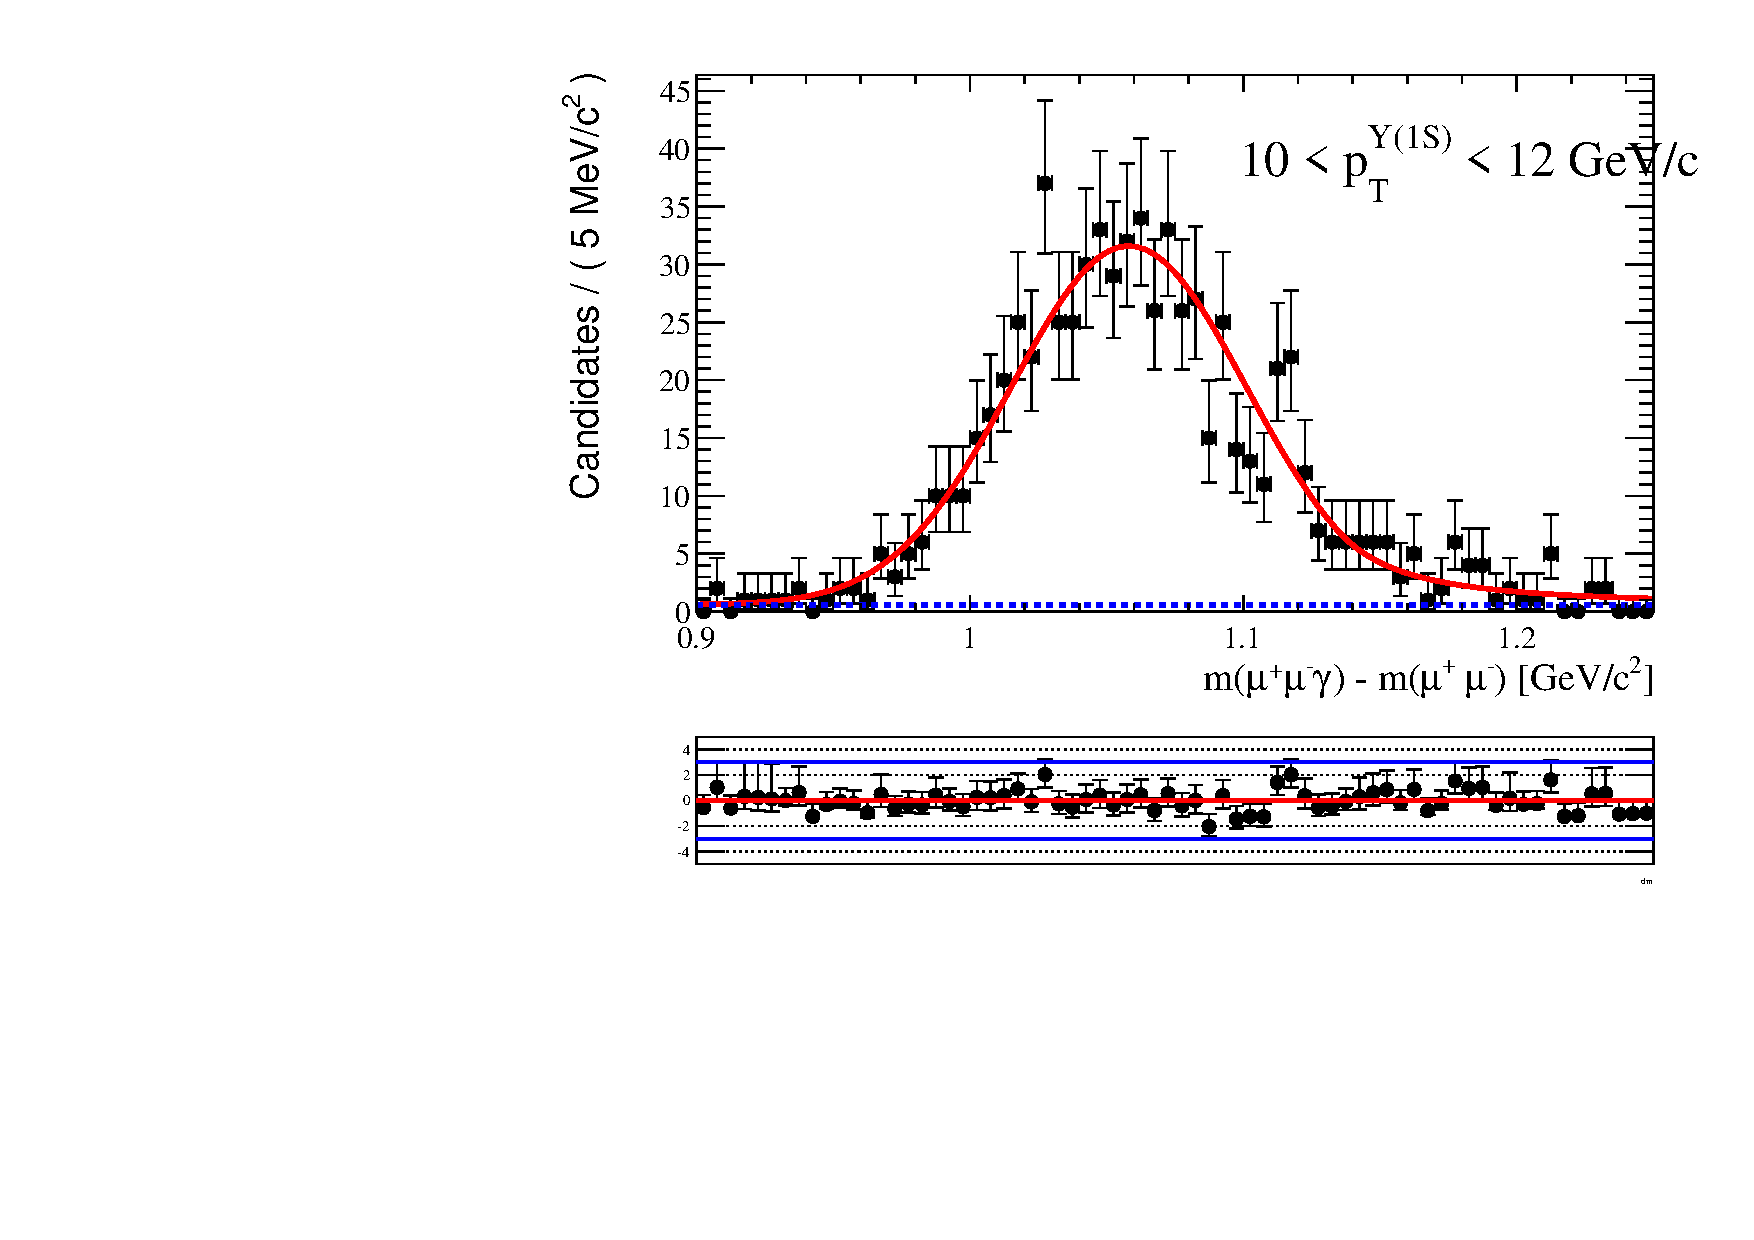
\includegraphics[width=0.16\linewidth]{fit_mc/chib23_10_12}
      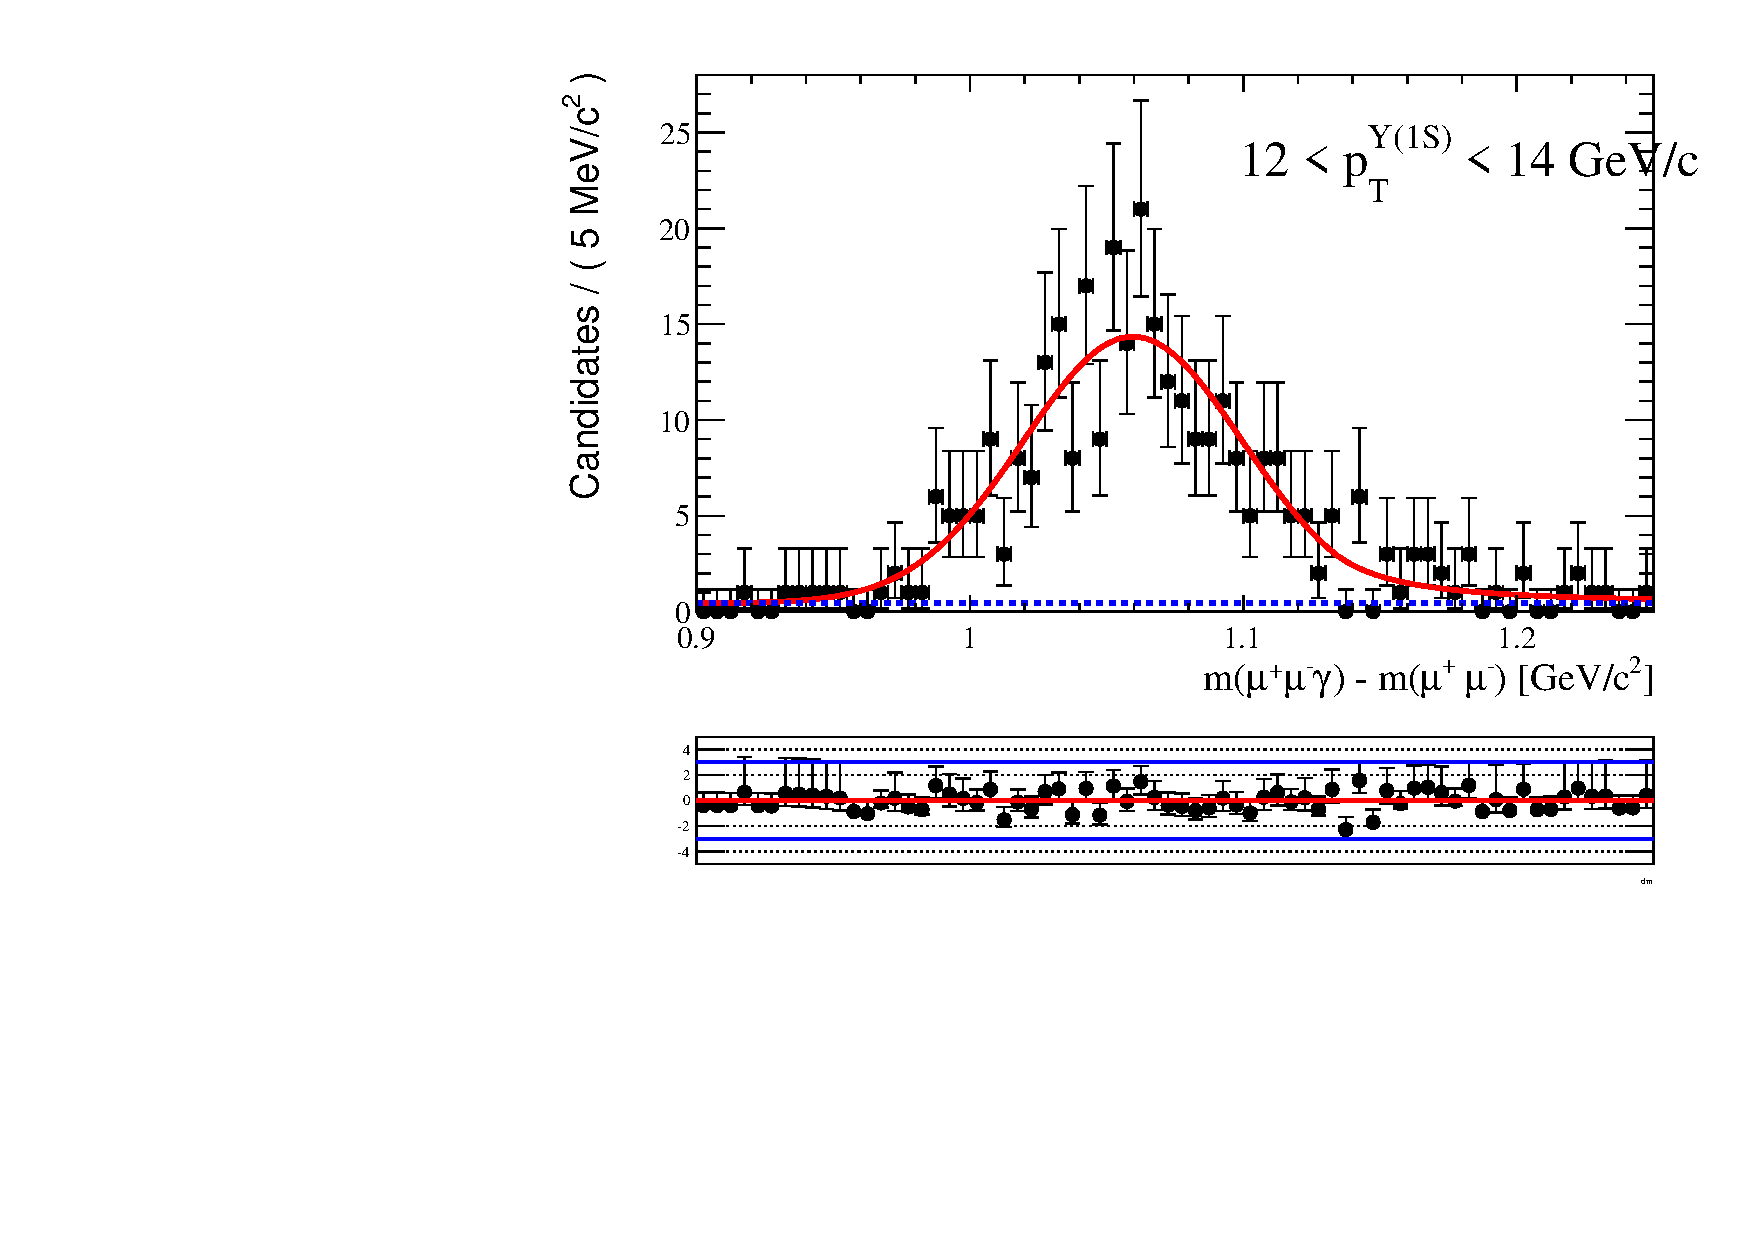
\includegraphics[width=0.16\linewidth]{fit_mc/chib23_12_14}
      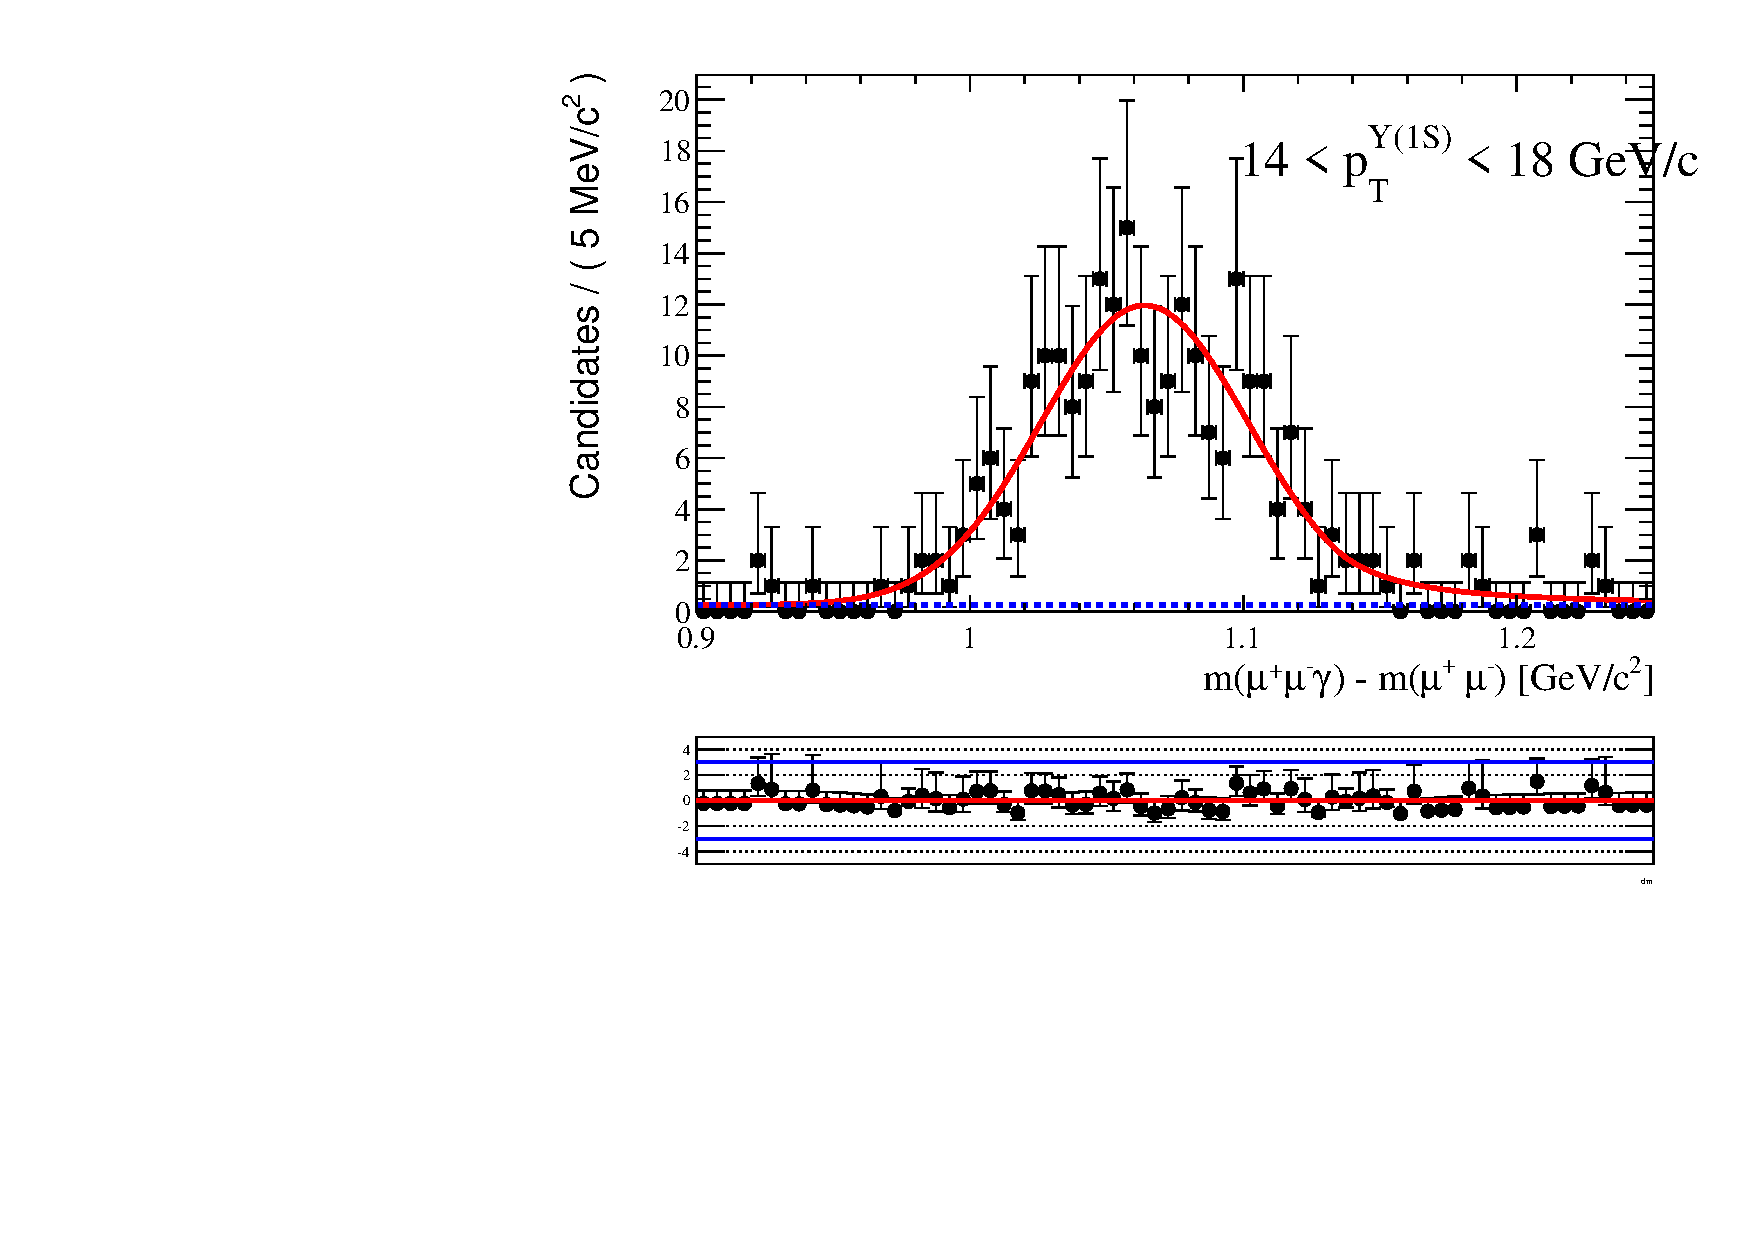
\includegraphics[width=0.16\linewidth]{fit_mc/chib23_14_18}
      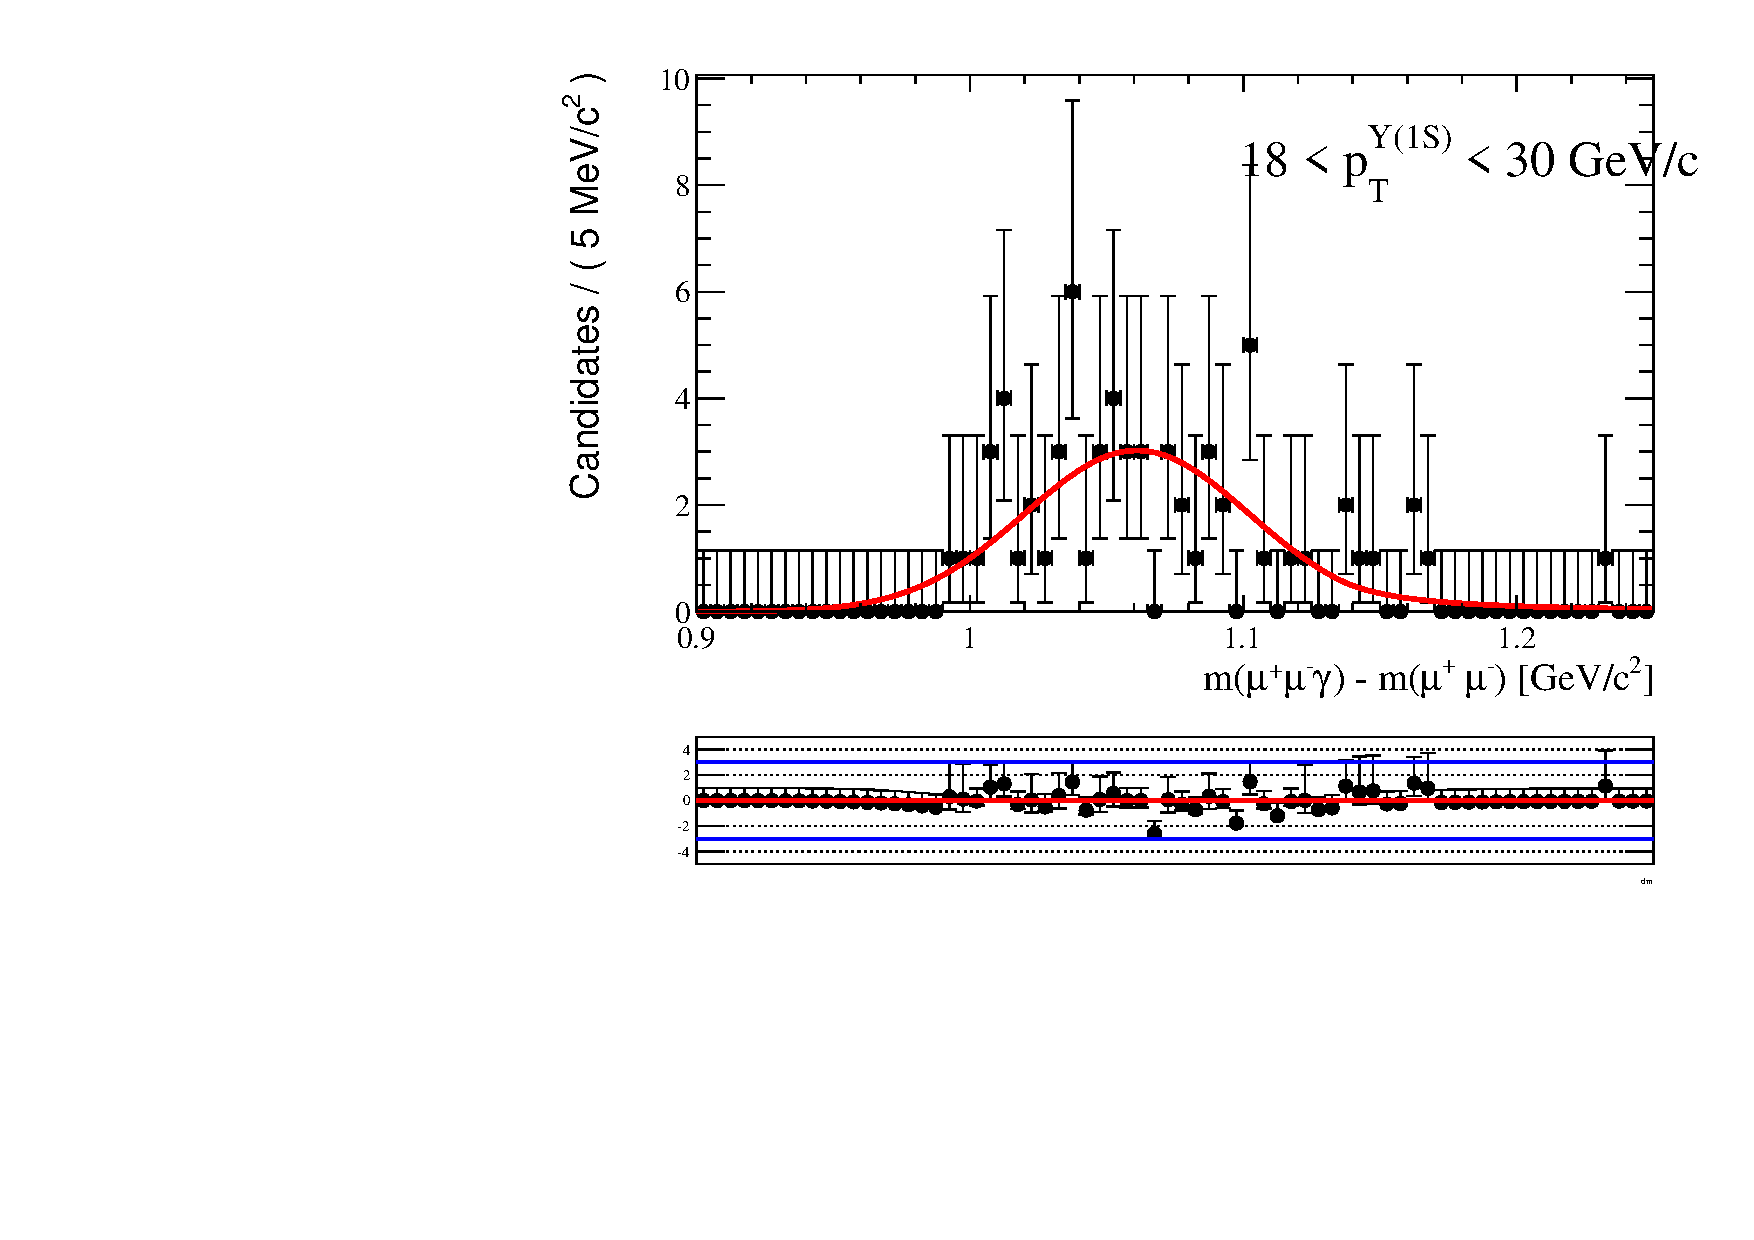
\includegraphics[width=0.16\linewidth]{fit_mc/chib23_18_30}
      \caption{\chibtwoThreeP}
      \label{fig:fit_mc_chibtwoThreeP}
    \end{subfigure}        
  \caption{
    \small  Mass difference of the $\mumu \gamma$ system and $\mumu$ system for the 
    Monte Carlo data for specified interval of transverse momentum of the \OneS. The red
    solid line is the result of the fit described in the text.
  }
  \label{fig:fit_mc}
\end{figure}